\documentclass[12pt,twoside, a4paper]{report}
\usepackage[T1]{fontenc}
%path [ansinew]{inputenc}
\usepackage[francais]{babel}
\usepackage{mathptmx}
\usepackage[french]{minitoc}
\usepackage[french, ruled, vlined]{algorithm2e}
\usepackage{graphicx}
\usepackage{makeidx}
\usepackage{lscape}
\usepackage[french]{algorithm2e} 
\usepackage{natbib}
\usepackage{here}
\usepackage{float}
\usepackage{hyperref}


%\usepackage{m2rinfo}
\usepackage{listings}
\usepackage{color}
\usepackage[utf8x]{inputenc}
\usepackage{geometry}
%\usepackage[authoryear]{natbib}
\geometry{verbose,tmargin=2cm,bmargin=2cm,
lmargin=3cm,rmargin=2cm,headsep=0cm}
%\usepackage[normalem]{ulem}
\usepackage[final]{pdfpages} 


\makeglossary

\begin{document}

%\paragraph*{\pagenumbering{Roman}}
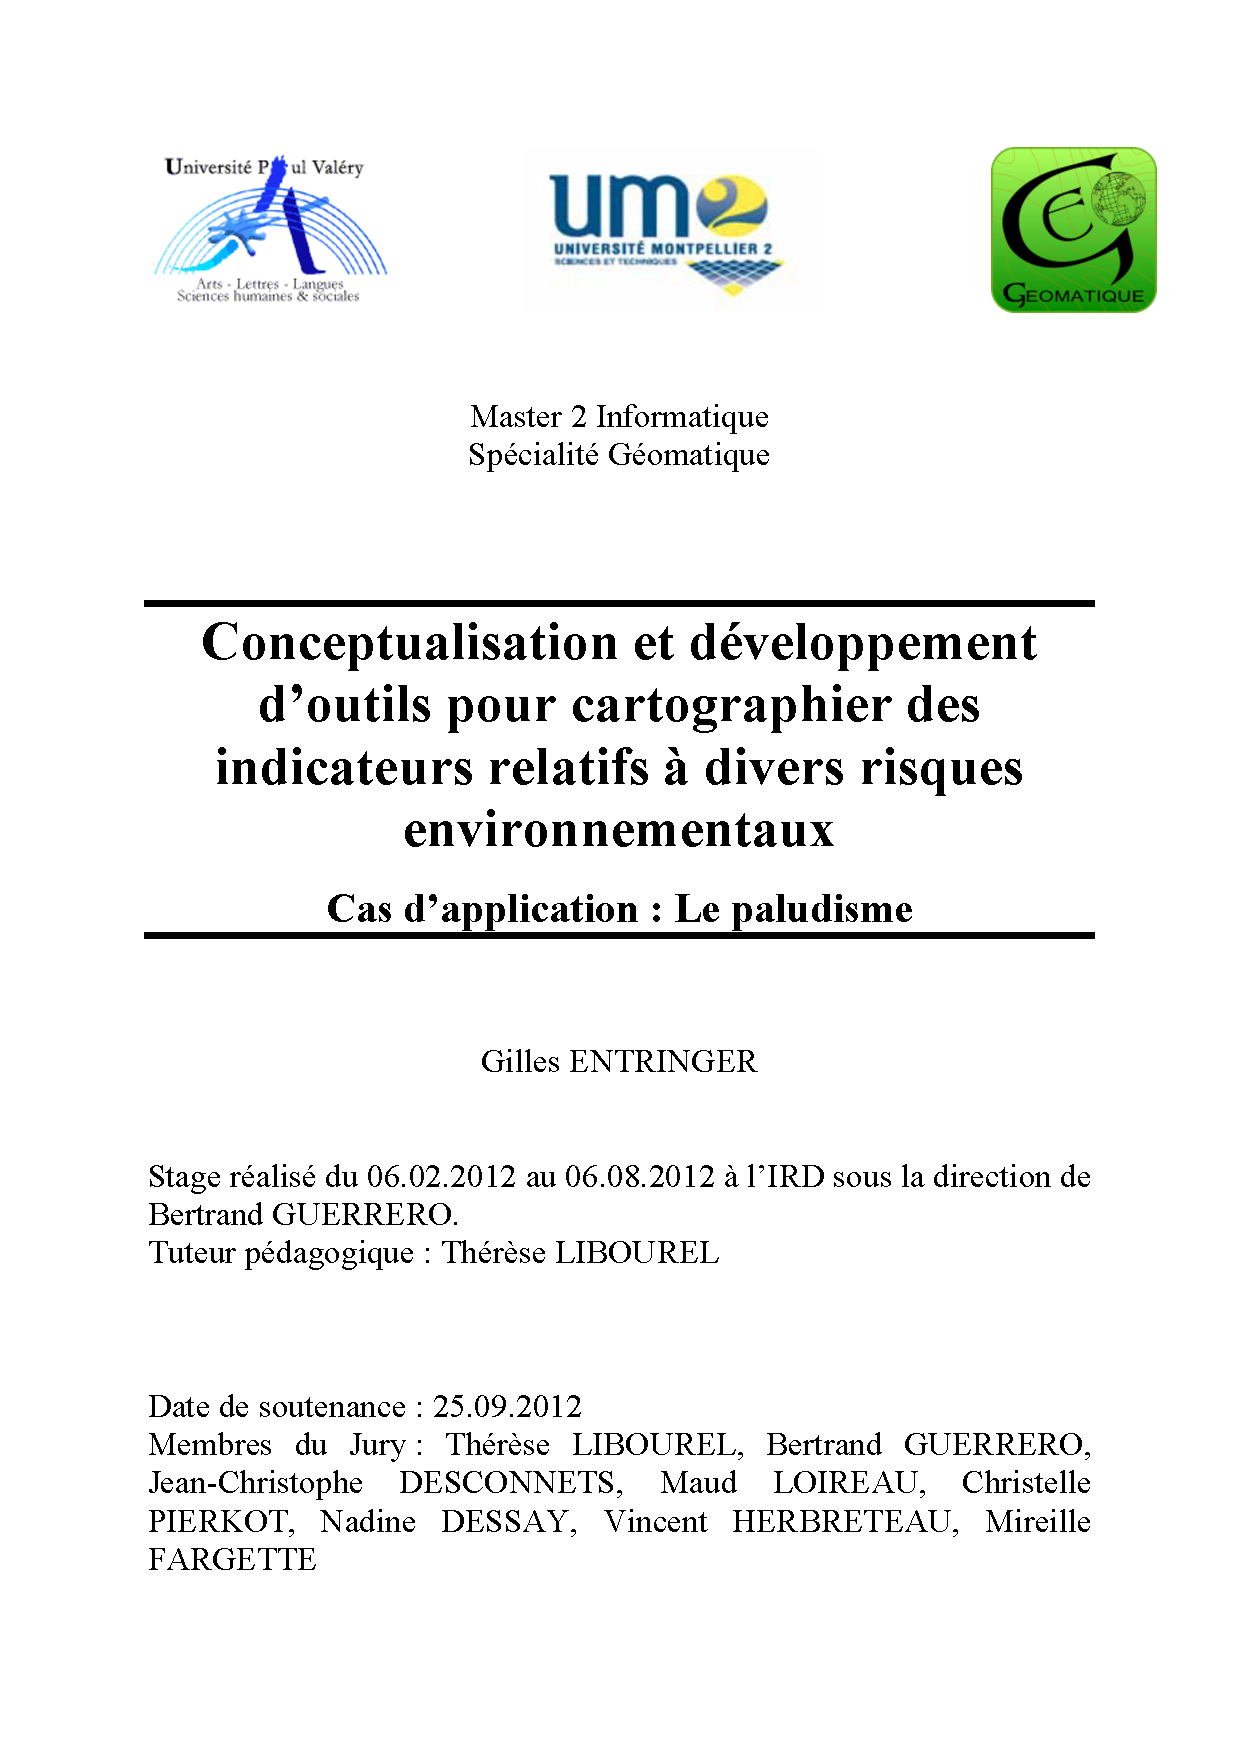
\includepdf{page_gardeM2.pdf}
\pagenumbering{roman} \setcounter{page}{1} 

\chapter*{Remerciements}
%\tableofcontents


Je tiens tout d’abord à remercier mon maître de stage Christophe Lapierre qui m’a permis de réaliser mon stage dans les meilleures conditions possibles. 
Je le remercie pour ses conseils, le temps qu’il m’a consacré et pour ses commentaires sur mon travail. \\

Je remercie Julien Lesbegueries pour m'avoir intégré dans son projet, m'avoir permis au cours du stage de découvrir des technologies telles que Dropwizard et pour toutes les bonnes pratiques de développement qu'il m'a transmises.\\

Merci à mes deux « super » formateurs Gilles Vanderstraeten (Java SE) et Laure Bouquety (Java EE), pour leurs cours et leur support, ils m'ont appris et fait aimer le langage Java. \\

Merci à Florian pour les pauses, et à Wafi pour ses dessins de réseaux sur mon bureau.\\

Enfin, je voudrais remercier particulièrement Frédéric Schettini de m’avoir donner cette opportunité de stage qui rentre pleinement dans mon projet professionnel, tant par les aspects techniques que par leurs domaines d'application. \\
 

\renewcommand{\contentsname}{Sommaire} %dans le corps du document, avant la commande \tableofcontents .

\tableofcontents


\pagenumbering{arabic} \setcounter{page}{1} 

\chapter{Introduction} 
\label{Introduction}

Ce stage s'inscrit dans le cadre de la formation "Concepteur / Développeur Informatique" délivrée par BGE Haute-Garonne et s'est déroulé durant 3 mois au sein de l'entreprise Mobigis. Les objectifs à l'issue de cette formation sont de savoir concevoir et développer des applications informatiques en utilisant le langage Java/JavaEE, dans un environnement professionnel.\\

Dans ce mémoire sera présenté le travail que j'ai réalisé, avec par exemple les résultats directs de mon action. Mais aussi, les tâches que j'ai effectuées et les moyens utilisés pour les accomplir : langages, frameworks, logiciels,…\\
 
Cette présentation s'organise de la façon suivante:\newline

\begin{itemize}
\item Une première partie sera dédiée à la présentation du contexte du stage. Dans cette partie seront présentés le domaine d'application de ce stage : les Systèmes d'Informations Géographiques (SIG), et l'entreprise MobiGIS.\\

\item Dans la deuxième partie, l'environnement de travail du stage sera expliqué : projets, équipes, outils, produits,...\\

\item Une troisième partie présentera la méthodologie de mon travail (conception/développement) et des exemples de réalisations (codes)...\\

\item Enfin, dans la dernière partie de ce mémoire seront présentés un bilan professionnel et un bilan personnel de cette nouvelle expérience.\newline

\end{itemize}

Par la suite, les termes en \textbf{gras} seront définis dans le glossaire en fin du mémoire.



\chapter{Contexte et problématique}



\section{Principes généraux}

%test \citealt{ref4}


A l'heure actuelle, le logiciel SIEL permet d'effectuer un certain nombre de traitements bien définis dans le contexte de la désertification et des risques de dégradation du sol. Le contexte environnement-santé est également une des préoccupations de l'UMR Espace-Dev et la réutilisation de cet outil, pour la création d'indicateurs du risque de transmission de maladies infectieuses, nous a apparu particulièrement intéressante. Afin d'optimiser et de généraliser cette réutilisabilité, il faut penser les chaînes de traitements dans ce nouveau contexte. \\

De plus, le SIEL est disponible en tant que plugin ArcGIS  et fonctionne avec des séries de traitements et d'opérations ciblées sur le type d'indice à produire. L'objectif à long terme est de retravailler ce logiciel pour qu'il devienne plus modulaire et générique, de préférence dans un contexte "Open Source". Nous avons donc décidé d'ouvrir l'outil et à repenser son architecture dans un contexte Open Source. \\

Dans ce contexte, la conception et le développement d'une chaîne de traitements liés aux indices santé-environnement avaient comme objectif de servir d'expérience préliminaire à la conception et à la réalisation d'une nouvelle architecture informatique du logiciel. %Le développement d'un \textbf{logiciel ouvert} a permis de franchir une étape supplémentaire dans le développement informatique du SIEL.
L'intégration de la création automatisée d'indicateurs dans le domaine environnement-santé constituera de plus, une première piste dans l'objectif plus large qui consiste à faire du SIEL un outil générique adaptable à divers autres contextes comme par exemple la déforestation.\\

Nous allons maintenant présenter brièvement le SIEL, ses principes, son architecture informatique et la chaîne de traitements qu'il exécute. Par la suite les problématiques du présent stage seront expliquées en détail.\\



%La définition des facteurs de risque est une autre étape indispensable de la conceptualisation et de l'élaboration de la chaîne de traitements. A partir d'un modèle du cycle de la malaria, des modèles de données et de traitements permettront de dégager les étapes nécessaire pour aboutir au résultat souhaité: un prototype d'une chaîne de traitements permettent de créer des cartes de risques du paludisme. A partir des données d'entrée choisies par l'utilisateur la chaîne calculera automatiquement les zones à risque de transmission du paludisme. Les résultats seront représentés sous forme de cartes.


\section{Le logiciel SIEL}

Le SIEL est un logiciel qui instrumente un modèle environnemental \citep{Loireau2007} spatialisant les pratiques d'exploitation des ressources sur un territoire, modélisant les paysages et évaluant les risques de dégradation des ressources.\\

Le SIEL est un outil conçu pour répondre aux besoins des scientifiques et décideurs concernés par la lutte contre la dégradation et la gestion des ressources naturelles. Le SIEL est capable d'anticiper les risques et de les suivre, ce qui est important notamment dans le cadre de la mise en place d'observatoires. Cet outil donne également la capacité aux scientifiques et aux décideurs de mesurer l'impact des opérations déjà effectuées sur un territoire et d'optimiser les actions futures notamment en terme de gestion des ressources  \citep{SIEL2012}.\\ 

Le logiciel a été conceptualisé à partir de 1993 par Maud Loireau dans le cadre de sa thèse. En même temps un premier prototype a été développé. En 2000, dans le cadre de la lutte contre la désertification, la démarche scientifique et le modèle général du SIEL ont été adoptés par le programme ROSELT \footnote{Réseau d'observatoires de Surveillance Ecologique à Long Terme} de l’OSS \footnote{Observatoire du Sahara et du Sahel}. Ceci a permis de développer un premier logiciel SIEL qui couvrait l'ensemble de la chaîne de traitements proposée. Une première version du logiciel traitant la ressource « végétation » a pu être déployée dans le réseau ROSELT/OSS dès la fin de l'année 2003.
A partir de 2006, les différents acteurs ont poursuivi les développements du logiciel. Ceci a débouché sur un logiciel opérationnel et prêt à être diffusé, une documentation (guide d'utilisateur, aide en ligne), une documentation technique (guide développeur, dictionnaire des données), une base de données exemple et des supports de formations. Actuellement, l'objectif principal reste le développement informatique du logiciel et le responsable du projet informatique est depuis 2010 Bertrand Guerrero.

%\subsection{Le "modèle" SIEL}
%
%
%Le SIEL se base sur le fonctionnement interactif milieux/sociétés sur un territoire dans lequel des acteurs, selon leurs représentations de leur territoire et leurs usages (agricole, pastoral, forestier), ont des pratiques qui permettent d'exploiter des ressources naturelles (physiques, biologiques) sur un territoire donné (Guide utilisateur). Les interactions entre l'espace, les acteurs, les usages et les ressources produisent des paysages qui vont composer les territoires. Ces paysages évoluent en fonction des interactions entre facteurs naturels et humains. 
%Pour mettre en œuvre ce phénomène, le modèle SIEL décompose le territoire en
%Unités Spatiales dites « de Référence » (USR). Ces USR correspondent à une délimitation
%spatiale des différents paysages du territoire par voie de modélisation.\\
%
%Un minimum de données est nécessaire pour alimenter la chaîne de traitements: 
%\begin{itemize}
%\item données socio-économiques (acteurs, stratégies, pratiques d'exploitation...)
%\item données biophysiques (ressources, végétation...)\\
%\end{itemize}
%
%Enfin, le modèle SIEL met en œuvre une méthode spatiale interdisciplinaire qui permet une cartographie dynamique des paysages et le calcul d'indices environnementaux associés \citep{Loireau2007}. 


\subsection{Architecture SIEL}

Le SIEL se présente sous forme d'un plugin ArcGIS et se base sur deux modules propriétaires:\\

\begin{itemize}
\item Module données (Logiciel Microsoft Access \textbf{SGBD}, langage de programmation : Visual Basic for Application (VBA)) pour la gestion et le stockage des tables attributaires (format .mdb).
\item Module SIG (Logiciel: ArcGIS Desktop avec l'extension Spatial Analyst, langage de programmation: Visual Basic 6.0 et langage ESRI ArcObjects) pour la gestion et le stockage des couches géographiques et les géotraitements.\\
\end{itemize}

Le système d'exploitation supporté est Windows XP, les logiciels supportés sont "Microsoft Office 2003" et "Microsoft Office 2007" pour le module données et "ArcGIS 9.1" et "ArcGIS 9.3" pour le module SIG. Les deux modules sont donc basés sur des outils propriétaires. Le SIEL a été développé en Visual Basic, langage informatique qui n'est plus supporté par les nouvelles versions d'ArcGIS ce qui cause un certain nombre de restrictions par rapport à son utilisation et le développement futur.

\subsection{Les chaînes de traitements du SIEL}

Les deux modules (Données et SIG), en faisant différents traitements, créent des \textbf{indices environnementaux spatialisés} qui permettent la cartographie des risques de dégradation des ressources. Les données utilisées et les résultats sont stockés dans une base de données Microsoft Access. 
% attention dire que ici on utilise le formalisme de Yuan et mettre ce formalisme 
% ensuite présenter les 3 chaines 
\begin{figure}[H]
\begin{center}
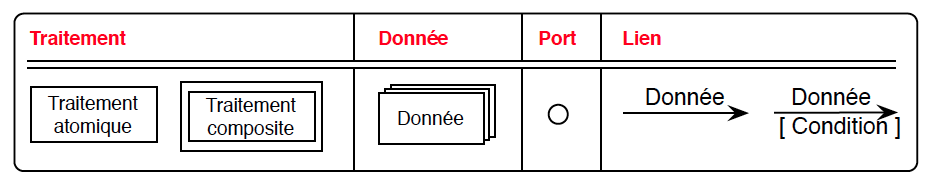
\includegraphics[width=16cm]{LinGraphique}\\
\caption{\label{LinGraph} Langage graphique proposé par Yuan Lin \citep{Lin2011}}
\end{center}
\end{figure}
A ce stade, nous utiliserons, pour formaliser les chaînes de traitements, le formalisme défini par Yuan Lin (cf. fig \ref{LinGraph}).

\paragraph{Description générale\\}

Le schéma \ref{SIEL1} explique de façon très simplifié le fonctionnement du SIEL. A partir de données statistiques et de données vectorielles le SIEL exécute des chaînes de traitements et fournit en sortie des indices de risque multi-usage.

\begin{center}
\begin{figure}[h] \centering
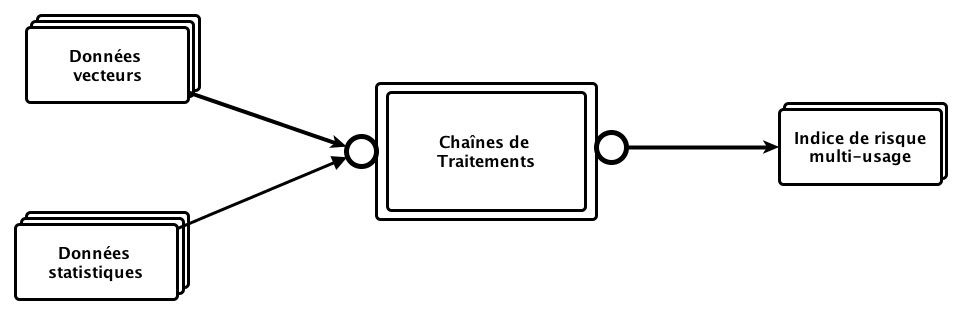
\includegraphics[width=16cm]{TraitementsSiel1.png}\\
\caption{\label{SIEL1} Description générale du SIEL}
\end{figure}
\end{center}

\paragraph{Chaîne de traitements abstraite\\}

Les traitements du SIEL peuvent être divisées en plusieurs sous-catégories: 

\begin{itemize}
\item Les traitements liés au territoire d'exploitation potentiel \footnote{Aire potentielle d’exploitation des ressources naturelles par un ou plusieurs groupes d’agents autour d’un centre d’activités, pour une période d’observation donnée. \citep{SIEL2012}}
\item Les traitements liés aux unités spatiales de référence \footnote{Une Unité Spatiale de Référence (USR) correspond à une délimitation spatiale d’un paysage par voie de modélisation \citep{SIEL2012}}
\item Les traitements liés aux indices de risque multi-usages

\end{itemize}

Les données d'entrée du SIEL sont des données vecteurs et des données statistiques. Au cours de l'exécution de la chaîne, des données intermédiaires sont également créées (au format raster, vecteur et statistique). 

\begin{center}
\begin{figure}[h] \centering
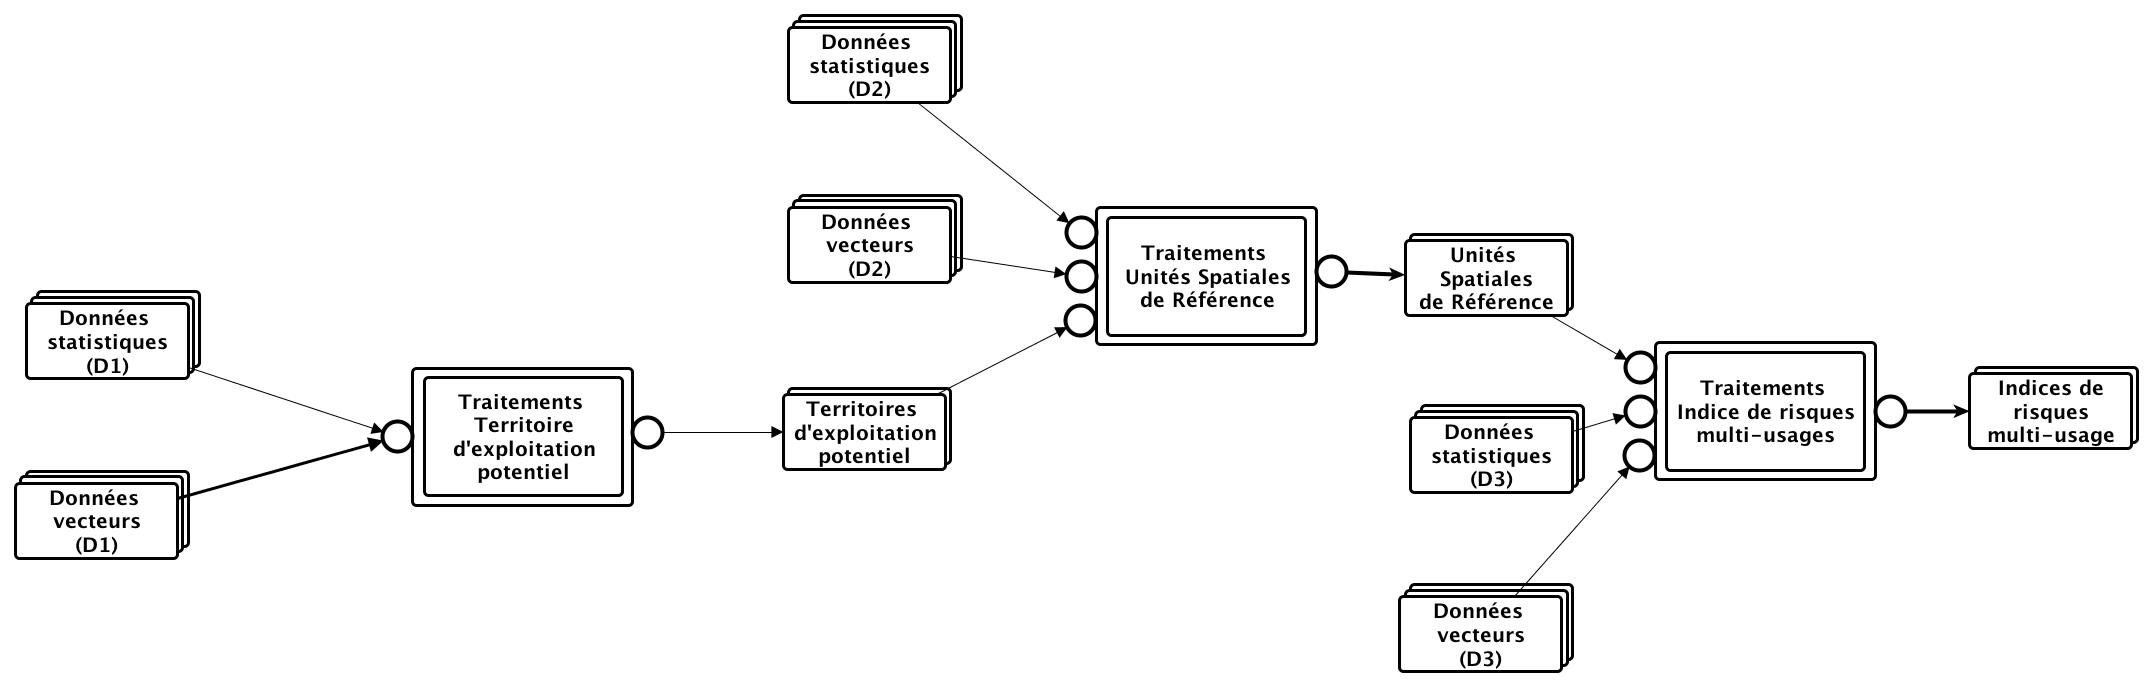
\includegraphics[width=16cm]{traitementsSiel2.png}\\
\caption{\label{SIEL2} Chaîne abstraite du SIEL}
\end{figure}
\end{center}

\newpage

\paragraph{Chaîne de traitements abstraite avec traitements élémentaires\\}

Le SIEL délimite dans un premier temps les territoires d'exploitation potentiels. Par la suite, le calcul des besoins et la spatialisation des pratiques permettent de délimiter les pratiques sur le territoire et plus précisément, à partir d'une intersection avec les unités paysagères, de créer des unités spatiales de référence.\\

A partir de différentes données d'entrée, le SIEL spatialise les prélèvement ce qui permet de déterminer les prélèvements en fonction de l'usage et de l'aire. Ce résultat temporaire et les unités spatiales de référence permettent finalement de calculer les indices de risque multi-usage en analysant l'usage par rapport aux prélèvements.

Les figures \ref{SIEL3} et \ref{SIEL4} montrent les traitements élémentaires du SIEL.





\begin{landscape}
\begin{figure}[h] \centering
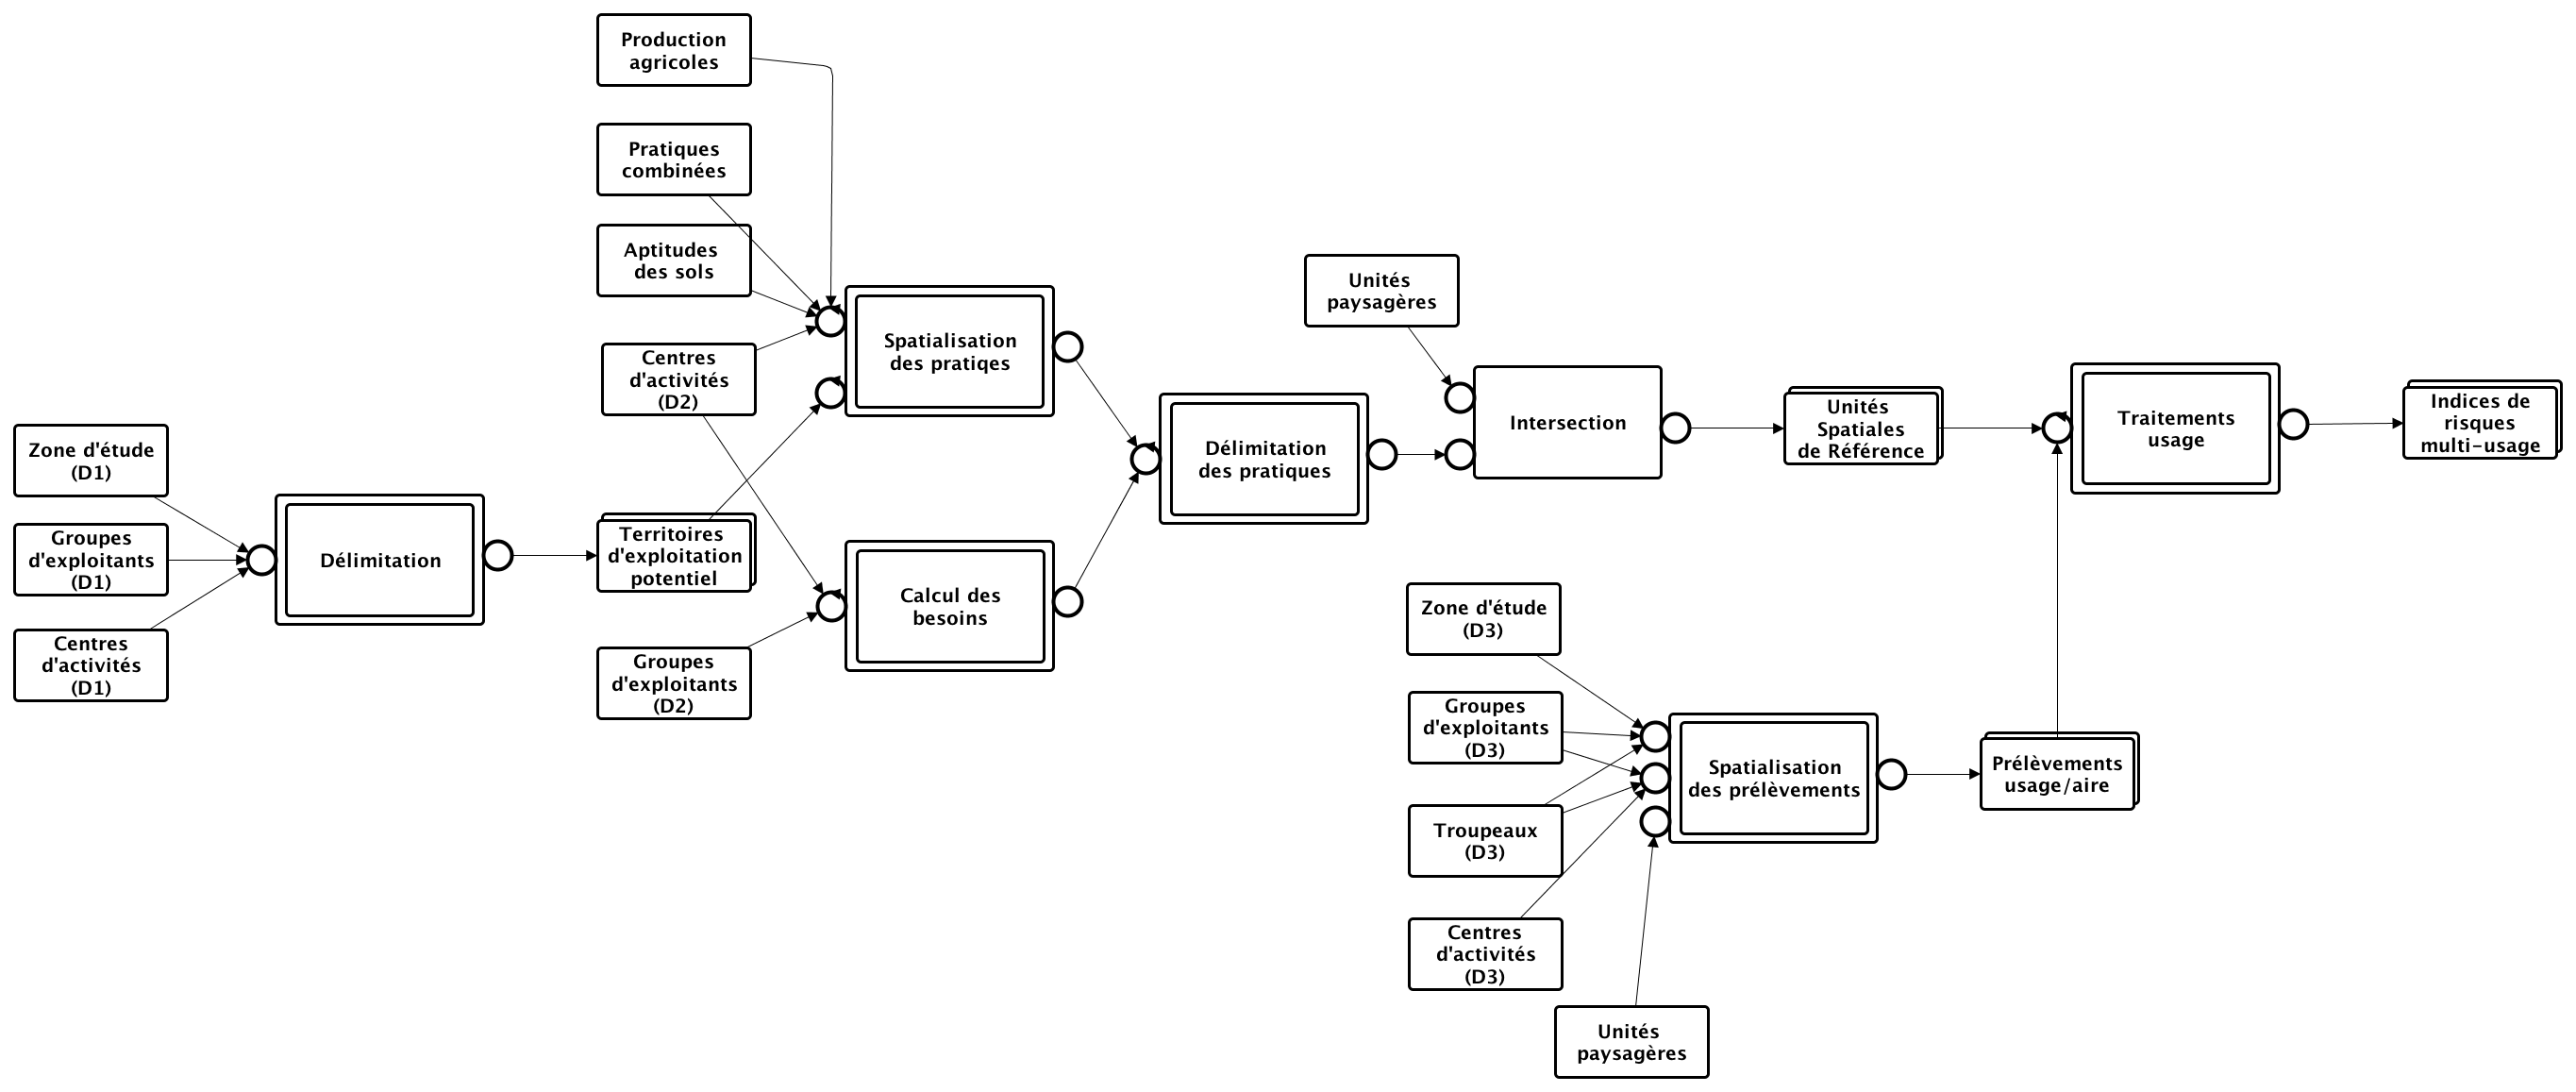
\includegraphics[width=23cm]{traitementsSiel3.png}\\
\caption{\label{SIEL3} Chaîne abstraite avec traitements élémentaires du SIEL}
\end{figure}
\end{landscape}

\begin{landscape}
\begin{figure}[h] \centering
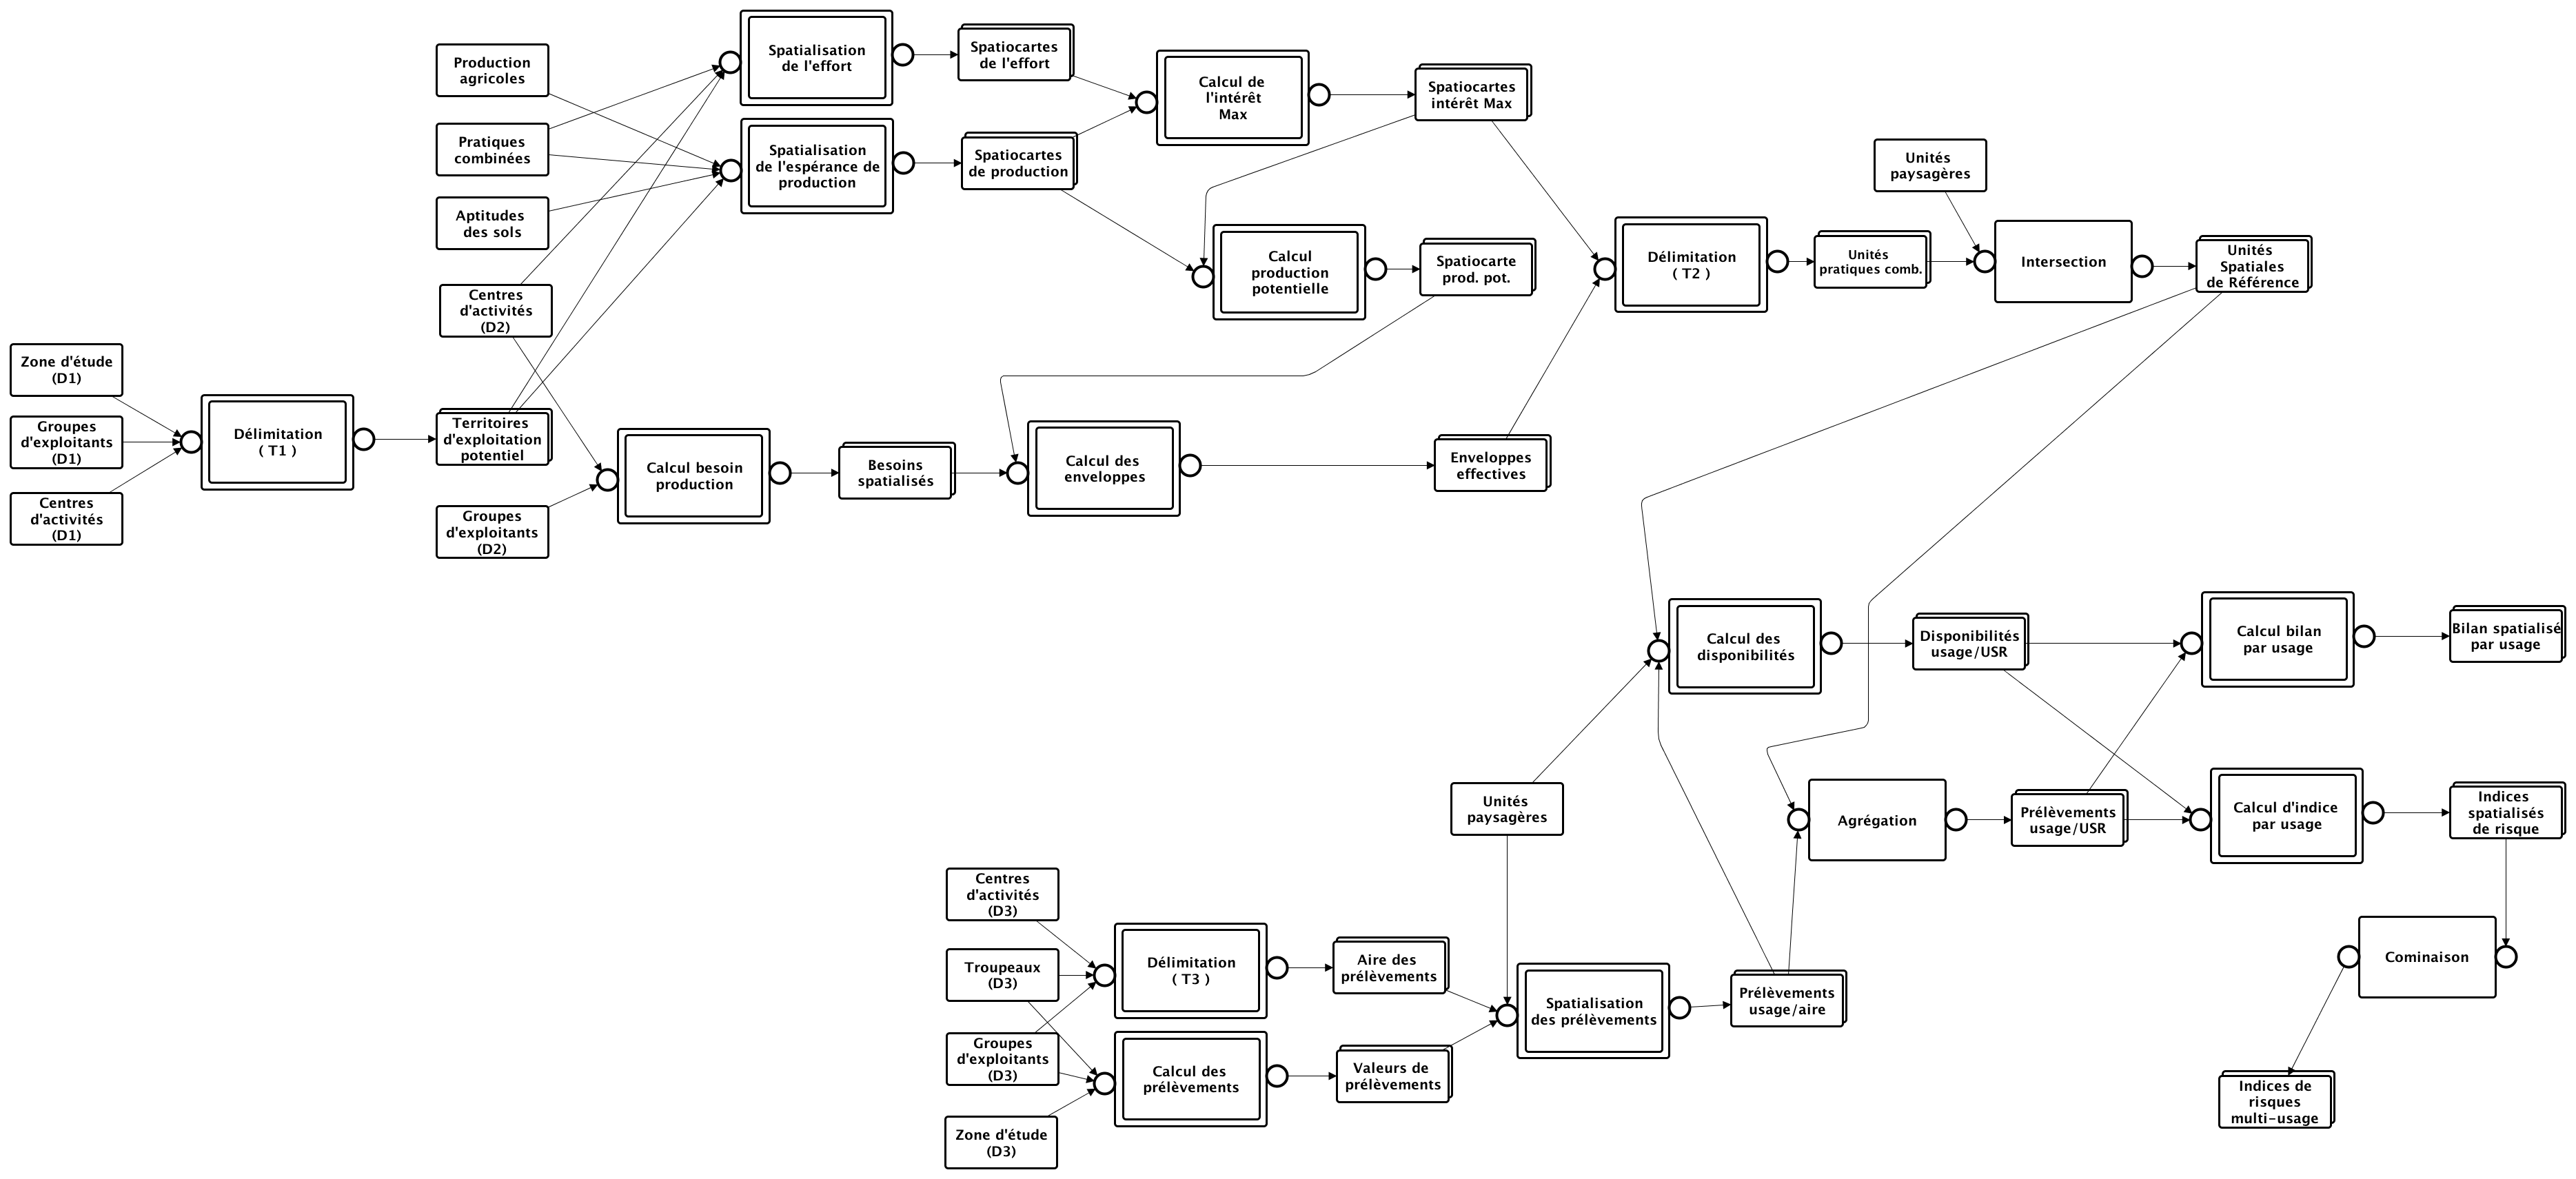
\includegraphics[width=23cm]{traitementsSiel4.png}\\
\caption{\label{SIEL4} Chaîne abstraite de plus en plus détaillée}
\end{figure}
\end{landscape}




%Suivi de phénomènes naturels ou anthropiques et l'orientation qui est choisi est de fabriquer des cartes révélatrices d'indicateurs pertinents.
%Exemple: désertifiaction (vulnérabilité à la désertification), déforestation
%Pour l'instant ce logiciel est un plugin ArcGIS et fonctionne avec des séries de traitements ou d'opérations ciblés sur le type d'indicateur à produire.

\newpage
\section{Problématiques du stage}


Étant donné la pluridisciplinarité du sujet de stage, les problématiques se regroupent en 2 catégories :\\
\begin{itemize}
\item Problématiques environnement-santé : Paludisme et les facteurs de risque de transmission
\item Problématiques informatiques : Conceptualisation des chaînes de traitements dans le contexte environnement-santé, choix de l'architecture et implémentation des outils (chaîne de traitements et logiciel ouvert).\\
\end{itemize}


Concernant le thème 'environnement-santé', la problématique principale est la compréhension du phénomène, la définition des facteurs de risque et la formalisation des éléments nécessaires à la mise en œuvre de la chaîne de traitements.\\

Au niveau informatique les points à traiter relèvent du choix de l'architecture informatique et de la réalisation d'un prototype de chaîne de traitements. Les principes de réutilisation et de généricité nous amènent à réfléchir sur une architecture "boîte blanche", qui consiste à ouvrir la boîte de la chaîne de traitements et à la déstructurer en boîtes élémentaires réutilisables. Le logiciel "ouvert" ainsi obtenu, permettra d'exécuter chaque traitement de la chaîne indépendamment les uns des autres et à les combiner selon les besoins de l'utilisateur.\\


%Le travail de Nadine Dessay sur l'élaboration de cartes de risques de paludisme va servir comme base lors de la définition des traitements à réaliser. Dans ce travail, elle définit les étapes nécessaires pour l'élaboration de ce type de cartes par rapport à la problématique du paludisme. Ces traitements sont réalisés sous ArcGIS, l'objectif est de trouver des fonctionnalités similaires avec des outils "OpenSource" et d'automatiser l'exécution de tous ces traitements et calculs à l'intérieur de la chaîne de traitements. Le logiciel ouvert permettra d'exécuter chacun de ces traitements indépendamment. \\
%
%
%Nadine Dessay a également extraits plusieurs données à partir d'une image de haute résolution \textbf{Quickbird} (...résolution) de la ville de Bandiagara au Mali qui serviront comme "données d'essai" pour le prototype de la chaîne de traitements.\\

En résumé la problématique générale du stage se dégage :\\ \textbf{Conceptualisation et développement d'outils pour cartographier des indicateurs relatifs à divers risques environnementaux.}
%
%L'idée est d'élargir les potentialités de cet outil afin de construire des indicateurs dans un contexte environnement-santé et de rendre le fonctionnement de cet outil plus souple, plus ouvert et donc faciliter son usage et son adaptation à divers contextes.




\chapter{Etat de l'art sur le thème environnement-santé} \label{Art}

Sans être exhaustifs, nous relatons ici, les principes relatifs au thème environnement-santé appliqué au paludisme, puis un rapide survol des logiciels et chaînes de traitements existants traitants d'indicateurs de risque épidémiologique.

\section{Interactions environnement-santé}

Je me suis focalisé dans un premier temps sur la définition des facteurs de risque de transmission dans le contexte des interactions environnement-santé et plus précisément dans le contexte de la maladie du paludisme. Dans une première partie les termes pertinents pour ce travail sont définis. Par la suite sont expliqués de façon détaillée les facteurs de risques de transmission identifiés à partir d'une recherche bibliographique.

\subsection{Définitions}


\subsubsection{Approche environnement-santé}

L'approche environnement-santé s'intéresse à l'influence de la qualité de l'environnement physique, chimique et biologique sur la santé des hommes et des animaux d'un point de vue spatial et dynamique. Il s'agit donc d'une science dont les frontières sont extrêmement difficiles à délimiter tant les domaines couverts sont  potentiellement vastes et susceptibles d'interférer les uns avec les autres \citep{afsset2006}.

\subsubsection{Paludisme}
Le paludisme, appelé également malaria, est une parasitose due à un protozoaire transmis par la piqûre de la femelle d'un moustique (\textbf{anophèle}), provoquant des fièvres intermittentes. Le paludisme est la maladie vectorielle la plus commune dans le monde avec une estimation de 216 millions de cas et 665000 décès en 2010 \citep{WHO2012} principalement dans les régions tropicales et en en Afrique sub-saharienne. Ces chiffres seraient bien inférieurs à l'étendue réelle de cette maladie, dont la mortalité est tout de même observée à la baisse grâce à l'action positive des programmes de contrôle (Murray et al, 2012).

Le médecin français Alphonse Laveran a découvert la cause de la maladie en 1880 à Constantine (Algérie). Le moustique anophèle se reproduit dans les zones marécageuses. Le parasite qui possède plusieurs hôtes intermédiaires, dans l'état endémique, infecte les cellules hépatiques de la victime puis circule dans le sang. Au cours de son cycle de vie, le parasite à l'intérieur de l'organisme humain, fait un certain nombre de transformations qui lui permettent d'échapper au système immunitaire humain. Au final, lorsqu'un moustique non-infecté pique une personne contaminée, le parasite est également transmis de l'homme au moustique.

En France et dans les autres pays développés, le paludisme a disparu depuis les années 1960. Malgré tout, depuis les années quatre-vingt les nombreux voyages effectués dans les pays où il est endémique, notamment dans les régions tropicales et subtropicales ont causé une réapparition de la maladie dans les pays développés.  

Actuellement, le paludisme est responsable de plus de 300 millions de cas de maladie aiguë et d'au moins un million de décès dans le monde. Quatre-vingt-dix pour cent des décès dus au paludisme surviennent en Afrique, au Sud du Sahara, principalement chez les jeunes enfants. De nos jours, aucun vaccin efficace n'a encore pu être développé et les scientifiques doutent de plus en plus qu'ils trouveront un jour la solution miracle contre cette maladie  \citep{questquelepaludisme}.

\subsubsection{Vulnérabilité}

La vulnérabilité dans le domaine de l'environnement-santé est la probabilité qu'une personne soit affectée (dans notre cas d'étude de la source d'une maladie) en fonction de sa susceptibilité aux effets de l'aléa et du niveau d'exposition. La précarité social et la vulnérabilité médicale sont étroitement associées et s'additionnent souvent \citep{DictionnaireSante}.

\subsubsection{Aléa}

Pour définir l'aléa pour le risque sanitaire, nous nous appuyons sur les travaux de \citep{Aschan2009}. Ces auteurs  définissent l'aléa comme une menace d'origine naturelle ou humaine sur un  système et distinguent deux  types d'aléas. Les perturbations sont des évènements ponctuels, repérables dans le temps, dont l'ampleur dépasse la variabilité habituelle du phénomène. Le « stress » est un autre type d'aléa qui exerce une pression continue sur le système, mais dont la variabilité est limitée.

\subsubsection{Risque}

Le risque peut être défini comme la combinaison entre l'aléa et la vulnérabilité. Le risque est la probabilité, aléatoire ou non d'un événement qui menace la santé ou met en danger la vie d'un individu ou d'une population. Le risque dépend de la capacité d'une population ou d'un système de faire face à des menaces (aléas). On peut distinguer des risques de nature différente: risques génétiques, risques naturels, risques anthropiques ou risques technologiques \citep{ORSN2010}.

En France et dans les pays de développement le paludisme a disparu parce que les responsables ont été capables de diminuer au minimum la vulnérabilité de la population et leur exposition au risque (en éradiquant les moustiques par exemple). 

D'autres notions associées au risque doivent être prises en compte dans l'analyse d'un risque sanitaire. La perception d'un risque donnée varie d'une personne à une autre, d'une société à une autre et conduit à des comportements protecteurs différents. Aussi l'enjeu du risque varie selon les personnes: être malade peut avoir des conséquences sociales et économiques graves pour un foyer, tout comme pour une société.

\subsubsection{Facteur de risque}
Un facteur de risque est la caractéristique individuelle ou collective, endogène ou exogène, augmentant de façon statistiquement significative la probabilité d'apparition et de développement d'une maladie. Un facteur de risque n'est donc pas une "cause". Il est également important de différencier facteur de risque et marqueur de risque (par exemple âge, sexe, groupe sanguin etc) car tout facteur de risque peut être contrôlé ou supprimé \citep{DictionnaireSante}.

Dans le cadre de cette étude, les facteurs de risques sont l'ensemble des éléments qui augmentent la probabilité que la  maladie (le paludisme) se développe sur un territoire. Un facteur de risque concerne donc aussi bien les aléas que la vulnérabilité. L'ampleur d'un risque , sa fréquence, sa durée, son aire d'extension et de diffusion éventuelle (espace à risque)à sont fonction de facteurs de risque.

\subsubsection{Indicateur}

Selon la norme ISO 8402, un indicateur est une "information choisie, associée à un phénomène, destinée à en observer périodiquement les évolutions au regard d'objectifs périodiquement définis". Un indicateur est donc une variable qui décrit un élément d'une situation ou une évolution d'un point de vue quantitatif. Un indicateur est un outil d'aide à la décision et n'a d'intérêt que par les choix qu'il aide à faire dans ce cadre \citep{ANAES2012}. 



\subsubsection{Carte de risque}

Une carte de risque permet de visualiser les zones de risque principales face à un "risque" spécifique. Une carte de risque est généralement obtenue en combinaison des cartes de vulnérabilité (par exemple densité de population) et des cartes d'aléas (par exemple proximité d'une surface d'eau ou de végétation dans le cas du paludisme). Ces cartes permettent, dans le futur, d'aménager le territoire de façon plus adapté au risque et de savoir par exemple, quels quartiers d'une ville sont particulièrement exposés à un risque. Une carte de risque permet de présenter de façon synthétique les risques. De telles cartes doivent être prudemment interprétées et utilisées et ne pas être distribuées sans explications. La façon de présenter et de discrétiser les données dans une carte peut conduire à de mauvaises interprétations.


\subsection{Facteurs de risque de transmission du paludisme}

En me basant sur une recherche bibliographique, j'ai élaboré une liste des différents facteurs causant respectivement le développement et la transmission du paludisme et qui sont susceptibles d'agrandir la vulnérabilité des habitants sur un territoire. Les facteurs peuvent être les mêmes pour d'autres maladies climato-dépendantes. Les facteurs sont regroupés en 3 catégories: Les facteurs liés à l'environnement, les facteurs biologiques et les facteurs humains. Les facteurs jouent un rôle plus ou moins important dans le développement du paludisme. Pour chaque catégorie un tableau présentera les différents facteurs. Chaque facteur sera par la suite expliqué en détail afin d'illustrer les caractéristiques spécifiques à chaque facteur de risque.

\newpage
\subsubsection{Facteurs environnementaux}
Les facteurs environnementaux sont en lien direct avec par exemple les conditions météorologiques ou avec la morphologie des sols sur un territoire. Toutes ces conditions vont influencer le risque que le paludisme puisse être transmis sur un territoire. \\

\begin{center}
\begin{tabular}{|c|c|} 
\hline
\textbf{Numéro} & \textbf{Facteur}\\
\hline
1 & Précipitation\\
\hline
2 & Température\\
\hline
3 & Distance au point d'eau le plus proche\\
\hline
4 & Caractéristiques du point d'eau\\
\hline
5 & Altitude\\
\hline
6 & Humidité\\
\hline
7 & Humidité du sol \\
\hline
8 & Température mois précédant les précipitations\\
\hline
9 & Végétation\\
\hline
\end{tabular}
\end{center}


\paragraph{Précipitation:}
Les précipitations sont parmi les facteurs de risque les plus important du paludisme puisqu'elle conditionnent l'écologie des moustiques, vecteurs des parasites. En examinant des territoires avec des cas de paludisme et des territoires sans cas de paludisme, il faut qu'il pleuve pendant 3 à 5 mois au moins 80 mm par mois pour que le paludisme puisse se développer \citep{Adjuik1998}. Les précipitations créent également des points d'eau temporaires, souvent difficilement repérables et idéaux pour le développement des moustiques. Ces points d'eau temporaires sont généralement de bonne qualité (non-pollués), ce qui est un autre facteur important.

\paragraph{Température:}

Le pourcentage de survie des moustiques sur un territoire est étroitement lié à la température \citep{Ermert2011}. Les moustiques disparaissent à partir d'une température de moins de 5°C et ne supportent pas des températures supérieures à 40°C. D'autres expériences montrent également que les moustiques ne peuvent pas survire les 56 jours de leur cycle de reproduction normal si les températures sont inférieures à 16°C et/ou supérieures à 32°C. La température idéale pour le cycle de reproduction du moustique est de 22°C. Dans ce cas-là, le cycle est fini après seulement 22 jours. \citep{Adjuik1998}

\paragraph{Distance point eau} 

Les moustiques anophèles peuvent se déplacer d'un maximum de 7 kilomètres par rapport à un point d'eau \citep{Ermert2011}. Les hommes habitant à plus de 7 kilomètres d'un point d'eau (de bonne qualité) ne sont donc, en théorie, exposés à aucun risque de paludisme. Néanmoins il est plutôt rare, notamment dans les pays en développement et donc dans les zones de risque majeures du paludisme que les gens habitent aussi éloigné d'un point d'eau. En plus, des expériences ont démontré que les moustiques infectés du paludisme peuvent être amenés par des voitures (par exemple) dans des zones non-vulnérables auparavant.

\paragraph{Caractéristiques du point eau} \label{caracteaux}
La surface et surtout la turbidité de l'eau jouent un rôle non négligeable dans le développement du paludisme. Lorsque le courant est trop fort, les œufs des moustiques sont lavés, les moustiques ne peuvent donc pas se reproduire. 
Des essais en laboratoire \citep{Minakawa1999} ont montré que les moustiques anophèles pondent plus d'œufs dans les points d'eau se situant sur des sols inondés ou humides que dans de l'eau "sans sol". En plus, les moustiques anophèles n'aiment pas, en général, les habitats ombragés tels que des réservoirs d'eau sans substrats de sol. En effet, le sol fournit des éléments nutritifs qui favorisent l'accumulation de bactéries qui sont la source de nourriture pour les larves.

\paragraph{Altitude}
L'altitude maximale retenue généralement est de 2000m. Ce facteur est bien évidemment étroitement lié au facteur de la température car la température diminue de 0.7°C tous les 100 mètres.

%\paragraph{NDVI}
%
%Le NDVI (normaized difference vegetation index) intègre et combine les effets de la température, humidité, précipiations et de l'altitude. Le NDVI varie entre -1 et +1 et se base sur l'optimum de...
%Rechercher définition scientifique.

\paragraph{Humidité de l'air}
L'humidité relative de l'air a un impact important sur la présence et la persistance des sites de reproduction des moustiques. Le taux de survie des moustiques est également influencé par ce facteur.

Le facteur peut être extrait à partir d'autres facteurs météorologiques comme les précipitations et la température mais doit être utilisé avec précaution . L'humidité est fortement influencée par la température de l'air et peut donc significativement changer pendant un seul jour. A noter que ce facteur dépend également de l'altitude. L'humidité idéale pour les moustiques est de 60 \% \citep{Protopopoff2009}.


\paragraph{Humidité du sol}
L'humidité du sol dépend directement des températures, de la végétation ou de la présence de points d'eau. Ce facteur est particulièrement intéressant car il peut être extrait à partir des images satellites. \citep{Machault2011}

\paragraph{Végétation:}

Certains types de végétation servent comme habitat pour les moustiques adultes.\citep{Minakawa1999} (à revoir)

\newpage

\subsubsection{Facteurs biologiques = marqueur de risque}

Les facteurs de risque de transmission biologiques sont liés par exemple à l'organisme humain ou à l'organisme du moustique. L'état de l'organisme humain, sous certaines conditions, peut augmenter le risque de l'apparition du paludisme sur un territoire. Certains de ces facteurs comme l'âge sont également des marqueurs de risque et ne peuvent pas être influencées respectivement modifiées.\\

\begin{center}

\begin{tabular}{|c|c|} 
\hline
\textbf{Numéro} & \textbf{Facteur}\\
\hline
1 & Etat de santé de la personne\\
\hline
2 & Densité du vecteur\\
\hline
3 & Transmission Homme-Moustique\\
\hline
4 & Immunité\\
\hline
5 & Age \\
\hline
\end{tabular}
\end{center}

\paragraph{État de santé de la personne}

L'état de santé de la personne joue un rôle majeur dans le développement du paludisme. Les personnes les plus en risque sont les enfants de moins de trois ans et les femmes enceintes et donc les personnes avec les systèmes immunitaires les plus fragiles. Les adultes ou les adolescents présentent généralement des systèmes immunitaires suffisamment puissants pour combattre le paludisme. 
\citep{Protopopoff2009}

\paragraph{Densité du vecteur}

Pour combattre le paludisme, il n'est pas nécessaire d'éradiquer complètement les moustiques sur le territoire mais il suffit de réduire la densité vectorielle \citep{Gaudart}. En général, la densité de l'anophèle diminue avec l'éloignement du gîte, avec la densité du tissu urbain et de la périphérie vers le centre \citep{Gaudart}. En analysant les densités vectorielles sur différents territoires, il est possible de déterminer les végétations ou écosystèmes les plus favorables pour le développement des larves.

\paragraph{Transmission Homme-Moustique}

En cas de piqûre, un humain porteur du parasite du paludisme transmet la maladie aux moustiques non-infectés par avant. Ceci est un autre facteur de risque à ne pas négliger, le taux de transmission est de 20\% (30\% pour une transmission moustique-homme).

\paragraph{Immunité} \label{immunite}
La capacité d'un organisme humain pour combattre l'infection du paludisme dépend de son immunité \citep{Protopopoff2009}. A partir de 2 à 3 ans, l'organisme humain développe et augmente l'immunité indépendamment du nombre de piqûres. Dans des régions avec peu de piqûres, le nombre de cas cliniques et d'infection est le même pour tous les groupes d'âge. Il faut donc que l'homme soit piqué régulièrement afin de développer une certaine immunité contre l'infection du paludisme.

\paragraph{Age}
Les enfants de moins de 3 ans sont piqués plus souvent, il semble que la proportion entre piqûres et un être humain soit liés à la taille du corps de l'hôte.  \citep{Ermert}

\subsubsection{Facteurs humains}
Les facteurs humains sont les facteurs liés à la présence humaine sur un territoire qui augmentent la vulnérabilité des habitants du territoire par rapport à la transmission du paludisme.

\begin{center}

\begin{tabular}{|c|c|} 
\hline
\textbf{Numéro} & \textbf{Facteur}\\
\hline
1 & Urbanisation \\
\hline
2 & Agriculture \\
\hline
3 & Qualité système santé \\
\hline
4 & Croissance démographique et Facteurs socio-économiques \\
\hline
\end{tabular}

\end{center}


\paragraph{Urbanisation}
L'urbanisation généralement diminue le risque du paludisme. Les points d'eau sont pollués, il y a peu de végétation etc. Ceci dépend malgré tout de la taille de l'urbanisation. Forcément, dans une grande ville le risque d'être piqué est moins grand car il y plus de "cibles" pour les moustiques, en même temps de nouveaux facteurs de risques peuvent apparaître comme par exemple les lumières et télévisions étant une source d'attraction pour les moustiques.

\paragraph{Agriculture / Irrigation}

Les activités agricoles influencent directement le risque du paludisme. Par exemple, en irriguant régulièrement les terres agricoles, ces surfaces (=surface d'eau temporaires et de bonne qualité) deviennent des endroits idéaux pour les moustiques pour pondre des œufs. La déforestation joue également sur le risque du paludisme. Des études récentes ont démontré que des habitations terrestres (des hommes) se situant en altitude, construits après une déforestation étaient des sites de reproduction préférés par les moustiques.\citep{Krefis2011}

\paragraph{Qualité système de santé}

La qualité du système de santé ou l'accès au système de santé influe directement sur le risque du paludisme  \citep{Protopopoff2009}. Des traitements préventifs permettent de réduire le taux de morbidité des femmes enceintes et des enfants, qui généralement ont le système immunitaire le plus fragile.


\paragraph{Croissance démographique / Facteurs socio-économiques}

Le statut socio-économique d'un individu est également d'importance. Les personnes les plus prospères sont capables de mieux se protéger contre les moustiques que les personnes très pauvres. Aussi, le niveau d'éducation peut influencer le risque de paludisme, Sachant que souvent les  personnes n'utilisent pas les filets anti-moustiques mis à leur disposition car ils ne comprennent pas vraiment le risque d'être piqués et le risque de paludisme, le niveau d'éducation des habitants est  également à prendre en compte.

Le type d'habitat de l'homme joue également un rôle important. En fonction du type d'habitat, le moustique peut entrer plus ou moins facilement dans l'habitat et piquer l'humain. Certains types d'habitations (en fonction du type de construction) peuvent même servir comme lieu d'habitat aux moustiques.


\subsubsection{Alea et Vulnérabilité selon les facteurs}

Les différents facteurs peuvent être regroupés en deux catégories différentes: les facteurs liés à l'aléa et les facteurs liés à la vulnérabilité. Certains facteurs peuvent créer un aléa et une vulnérabilité en même temps. Par exemple, en irriguant des terres, les agriculteurs créent involontairement un aléa (en créant des points d'eau temporaires) et aggravent en même temps la vulnérabilité des habitants du territoire. La figure \ref{AleaVuln} récapitule quels facteurs peuvent être à la base d'un aléa et lesquels peuvent aggraver la vulnérabilité.\\

\newpage

\begin{figure}[H]
\begin{center}

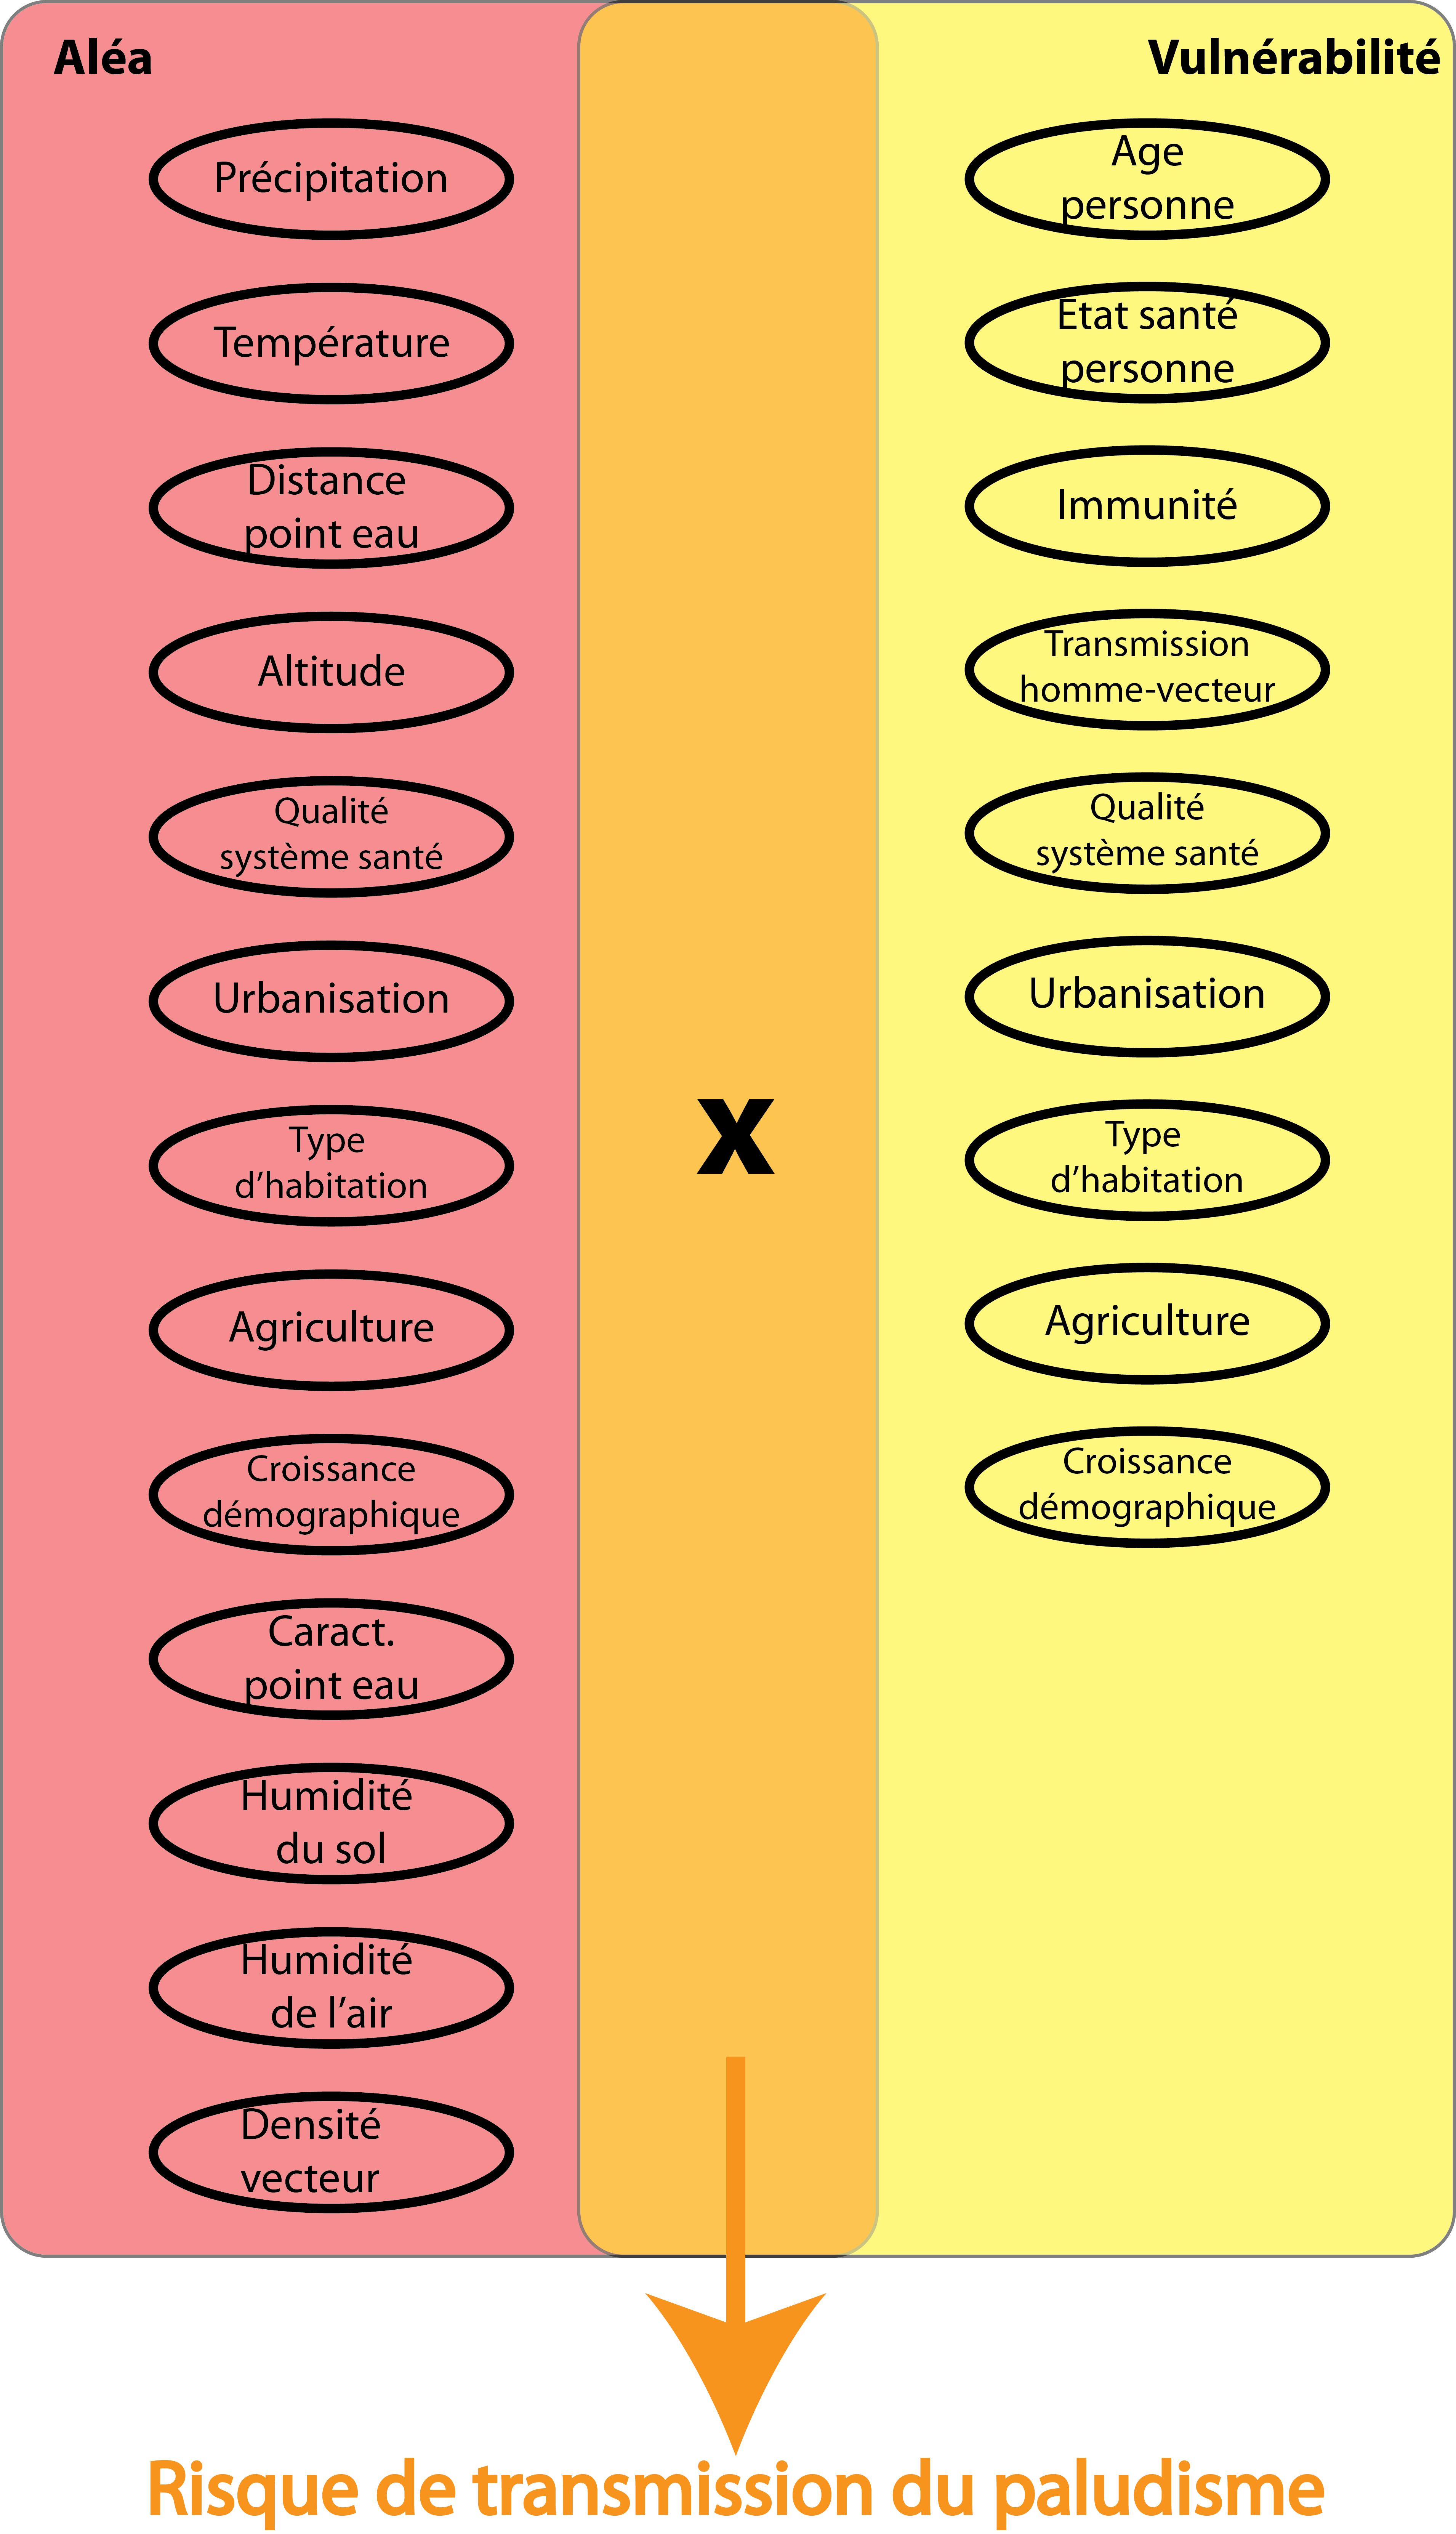
\includegraphics[width=9cm]{AleaVulnerab.png}\\
\caption{\label{AleaVuln} Alea et Vulnérabilité selon les facteurs}
\end{center}

\end{figure}


\section{Approches logicielles existantes}

Nous nous sommes simultanément intéressés aux logiciels et aux chaînes de traitements existants qui traitent les mêmes problématiques et / ou des problématiques similaires. Je présenterai dans cette partie du mémoire les approches logicielles que j'ai pu découvrir en faisant des recherches.

Nous avons focalisé nos recherches sur des outils qui se basent sur le principe d'analyse par rapport à l'existence de certaines variables (par exemple présence de points d'eau sur un territoire). Un autre principe d'analyse aurait été de définir le risque à travers l'absence de certaines variables (par exemple pas de végétation à proximité des lieux d'habitation des population).


\subsubsection{Repast Simphony}
Repast Simphony est une plate-forme de modélisation basée sur \textbf{Java}. Repast Simphony est un plugin \textbf{Eclipse} et permet de développer des programmes avec de nombreuses interactions. Repast Symphony a déjà été utilisé dans de nombreux domaines, comme en sciences sociales ou en sciences humaines. 


\subsubsection{Maxent}
Maxent est un logiciel gratuit qui permet de prédire la distribution potentielle (modélisation de l'habitat) des espèces animales ou végétales en se basant sur la distribution ponctuelle et certains facteurs environnementaux des espèces.

L'outil utilise comme variables d'entrée des données géoréférencées  des animaux respectivement de la végétation à modéliser et des données appropriées aux variables environnementales (par exemple pluviométrie, température, topographie etc.) au format ASCII (format ESRI). La modélisation est basée sur la méthode de l'entropie maximum. L'outil livre en tant que résultat une carte indiquant l'apparition potentielle des espèces ainsi que d'autres résultats statistiques. La visualisation des résultats se fait à l'aide d'un système d'information géographique. L'outil a été développé en Java et est disponible pour tous les systèmes d'exploitation.

\subsubsection{OpenModeller}

OpenModeller vise à fournir un environnement multi-plateformes permettant la réalisation de l'ensemble  du processus de "\textbf{niches fondamentales}". 
Le logiciel  facilite la lecture de l'occurrence des espèces et des données environnementales, la sélection des couches de données environnementales, la création d'un modèle de niche fondamentale et la projection du modèle dans un scénario de l'environnement. Un certain nombre d'algorithmes est également fourni sous forme de plugins et le logiciel permettant notamment de générer plusieurs modèles en utilisant différents
algorithmes face à une même problématique. Le projet est Open Source, multi-plateforme et développé en C++.


\subsection{Cas d'utilisation concret dans le contexte environnement-santé:}

\subsubsection{Le projet SimMasto}

Le projet SimMasto s'inscrit dans le cadre d'un projet de recherche sur la dynamique des populations de rongeurs. Il vise à développer une plate-forme générique de simulation des rongeurs dans leur environnement. Les données utilisées sont des cartes géographiques numériques, des cartes raster, des grilles théoriques etc.
La chaîne de traitements qui a été développée comprend les éléments permettant le traitement des images d'entrée (géoréférencement, détourage, changement de résolution, clipping, etc.) ainsi que tous les éléments de programmation nécessaires.

La chaîne de traitements est composée de plusieurs "modules", comme par exemple:
\begin{itemize}
\item Géoréférencement d'une image de type raster
\item Vectorisation d'une image de type raster (utilisation de la librairie Grass)
\item Modification du système de coordonnées
\end{itemize}

La chaîne de traitements fait par la suite appel à Repast Symphony pour mettre en place une simulation. Dans Repast Symphony est implanté un SIG, c'est-à-dire les différents fichiers de formes géoréférencés créés par avant ainsi qu'un fichier raster (une grille). D'autres outils / bibliothèques utilisés dans cette chaîne de traitements sont par exemples \textbf{PostgreSQL} / \textbf{PostGIS} ou \textbf{Eclipse}.


\section{Conclusion}

Dans le contexte choisi de l'environnement-santé, le premier travail a consisté à s'approprier la terminologie et à rechercher les outils logiciels existants.

Nous disposons des différentes définitions clairement établies, par contre sur le volet informatique, aucun outil ne semble proposer la solution attendue. En effet il n'existe pas, à notre connaissance et à ce jour, de chaîne de traitements automatisée permettant de cartographier facilement les zones de risque du paludisme. 

Il est donc particulièrement intéressant de proposer des prototypes d'outils permettant de cartographier les indicateurs relatifs à divers risques environnementaux. 



\chapter{Méthodologie} \label{Methodologie}

L'objectif principal du stage est de proposer un outil et une architecture logicielle permettant d'automatiser les \textbf{traitements} nécessaires pour cartographier le risque dans le contexte du paludisme (environnement-santé). Calculer le risque ou les indicateurs revient à définir des chaînes de traitements. Celles-ci sont conceptualisées à partir de l'expertise du domaine.\\


Une première partie d'analyse est dédiée à la compréhension du phénomène (paludisme) et à la conceptualisation des chaînes de traitements. Un modèle conceptuel UML des éléments nécessaires à l'élaboration des indicateurs permet de dégager les facteurs de risque les plus pertinents. A partir des données disponibles, un deuxième modèle UML simplifié servira comme base pour la définition des traitements nécessaires à l'élaboration et au développement de la chaîne. Dans un second temps, des \textbf{modèles conceptuels} des traitements permettent de d'analyser et de définir les différentes étapes nécessaires pour le développement informatique.\\ 

Dans une deuxième partie nous présentons l'architecture informatique des outils ainsi que tout le travail de conception mené autour du développement informatique.\\

Finalement, nous présentons l'opérationnalisation et l'implémentation des deux outils.


\section{Analyse}

Le cycle du paludisme (\ref{cyclemalaria}) permet de comprendre de façon simplifié le développement du paludisme. Ce qui est le plus important à retenir est que le moustique (qui a son propre cycle de développement) pique et infecte l'homme et les parasites se développent dans le foie et le sang de l'homme. Par la suite, un homme porteur du parasite piqué par un moustique sain, infecte celui-ci. Le cycle est donc complexe.


\begin{center}
\begin{figure}[h] \centering
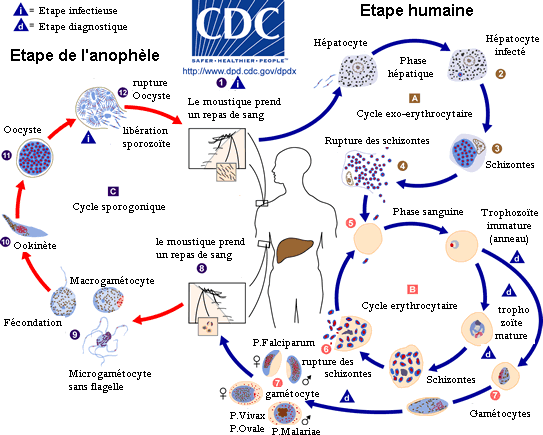
\includegraphics[width=14cm]{malaria}\\
\caption{\label{cyclemalaria} Cycle du paludisme (Extrait de  http://fr.wikipedia.org/wiki/Fichier:Malaria\_LifeCycle)}
\end{figure}
\end{center}

\newpage

\paragraph{Modèle conceptuel des éléments nécessaires à l'élaboration des indicateurs\\\\}
Le modèle conceptuel des éléments nécessaires à l'élaboration des indicateurs (\ref{UML_malaria}) permet d'avoir une vue d'ensemble des facteurs qui interviennent dans le développement du paludisme et qui peuvent être une source de risque. Les grandes caractéristiques du paludisme ont été définies dans une démarche participative lors d'une réunion avec des experts de différents domaines. A partir de ces caractéristiques j'ai élaboré un modèle conceptuel UML.\\

\newpage

\begin{landscape}
\begin{figure}[h]
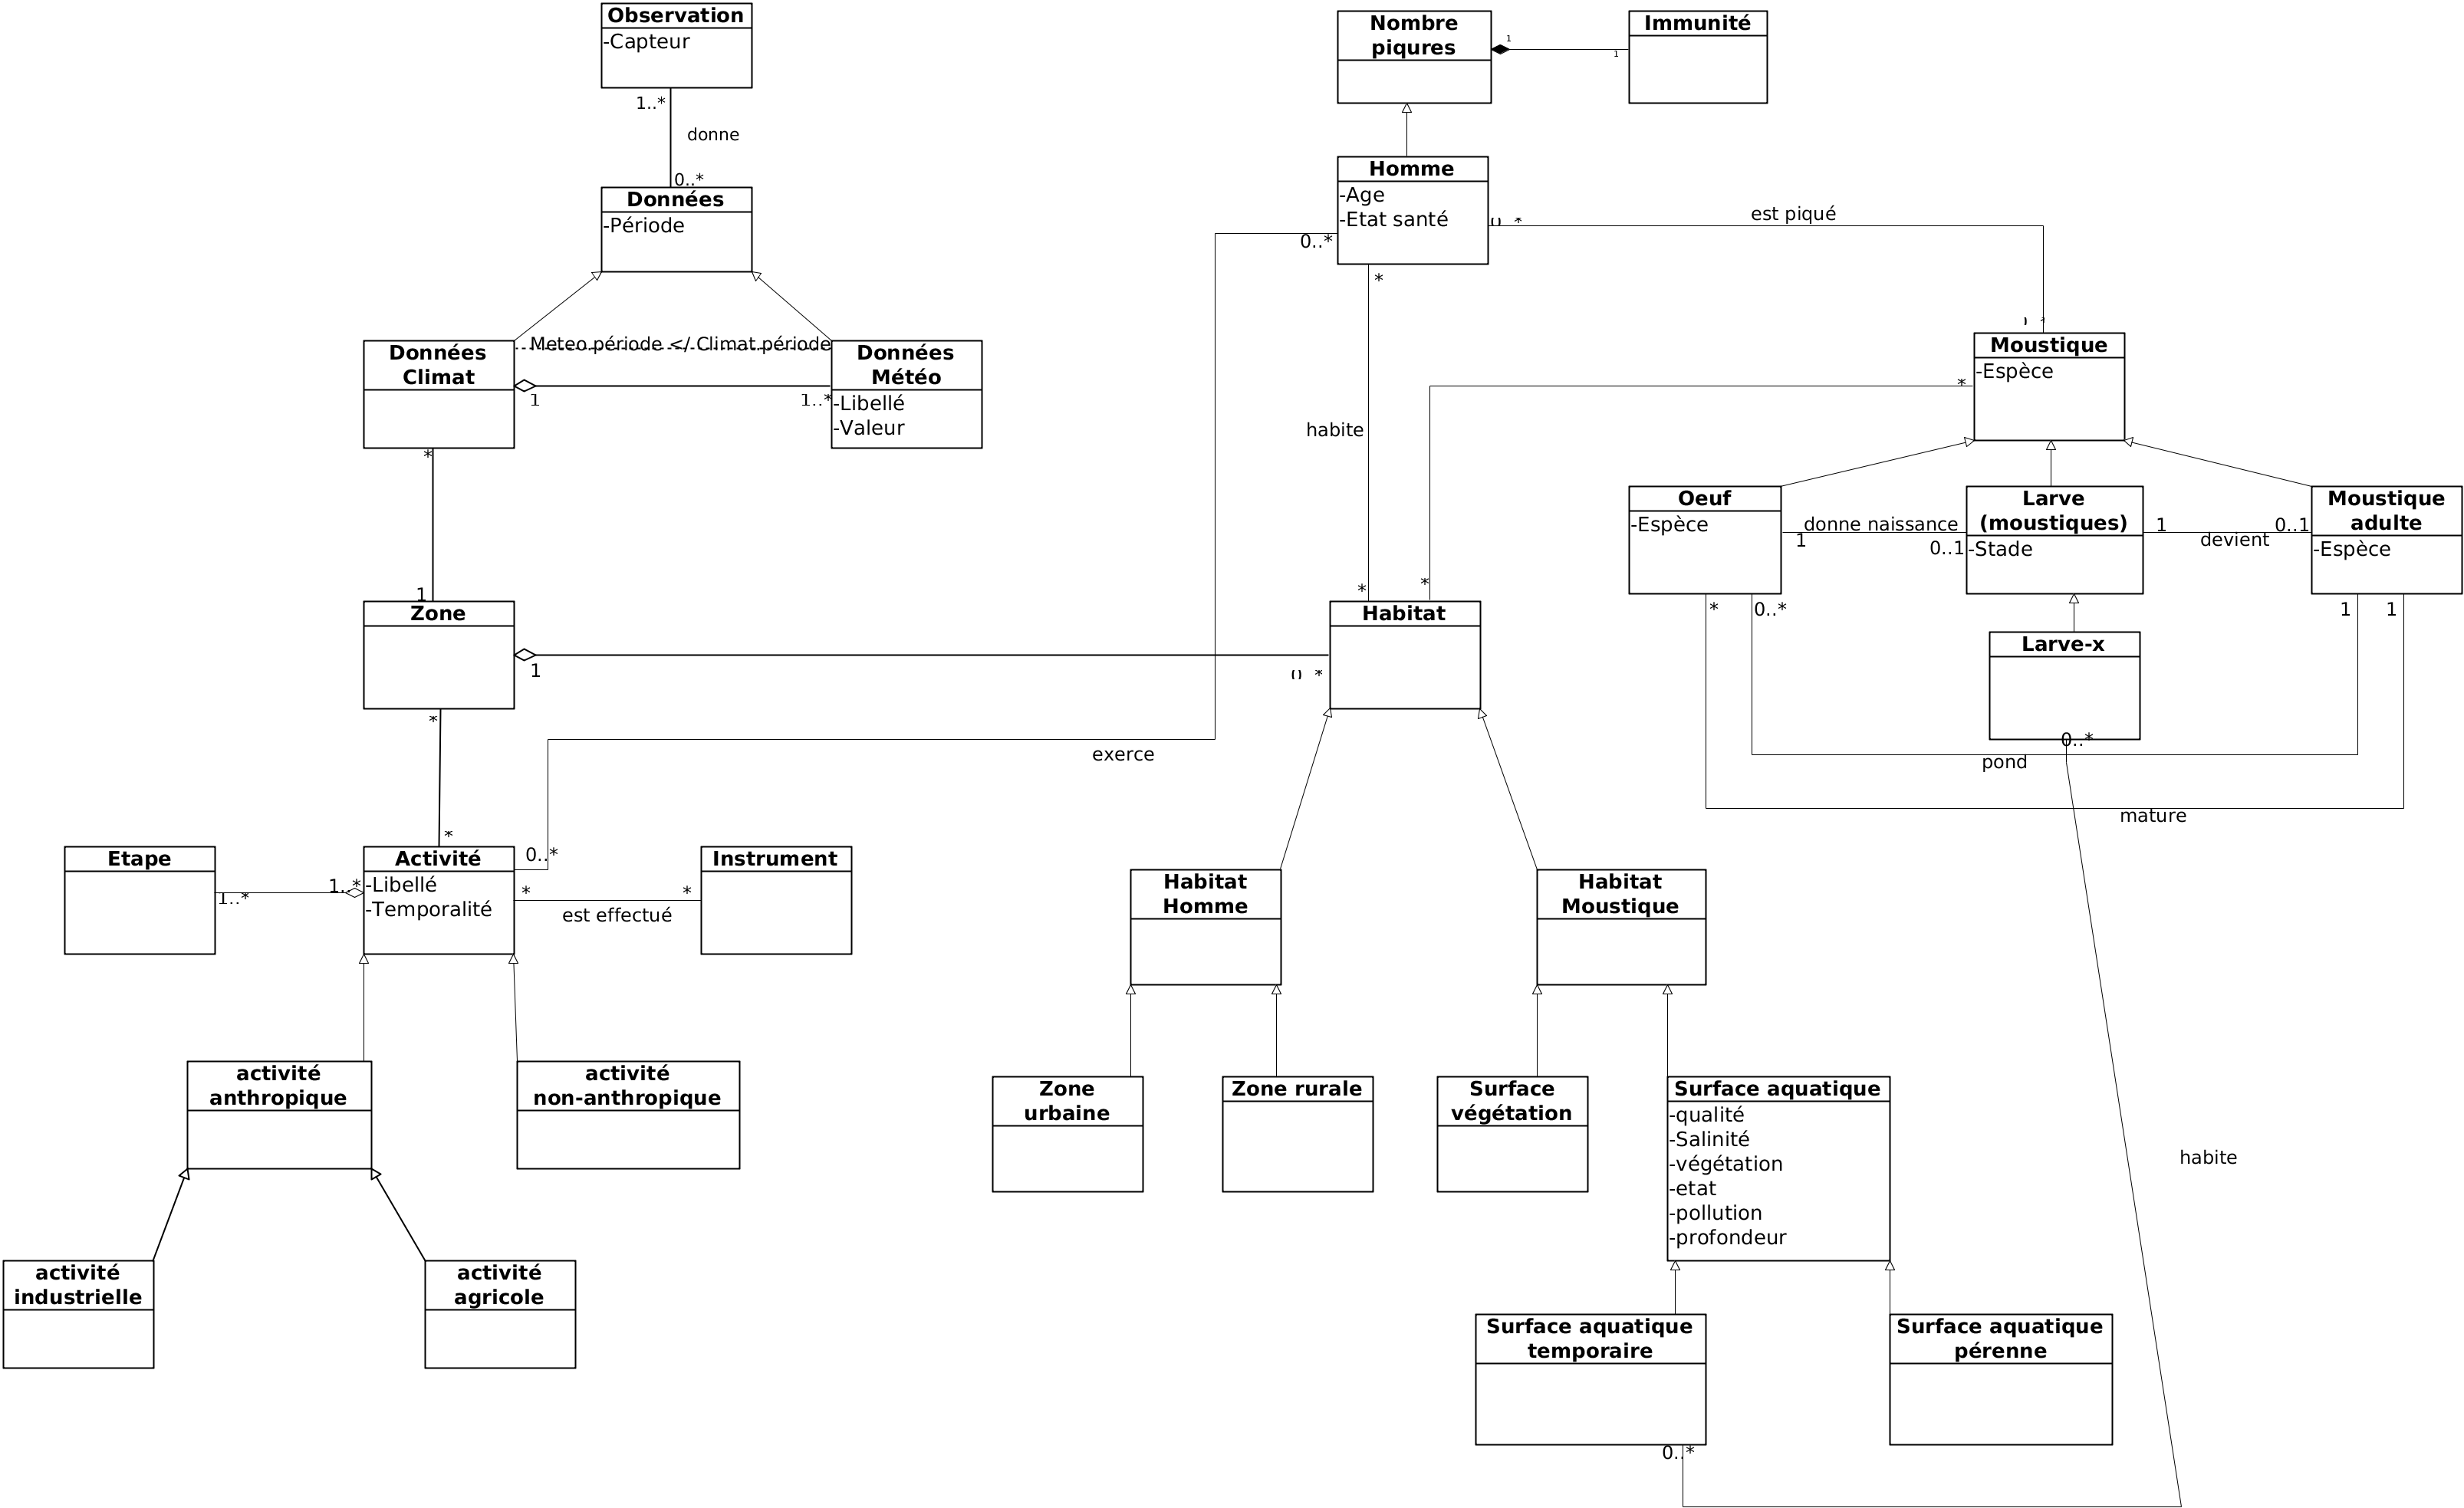
\includegraphics[width=23cm]{DiagrammeUML}\\
\caption{\label{UML_malaria} Modèle conceptuel UML des éléments nécessaires à l'élaboration des indicateurs}
\end{figure}
\end{landscape}

\subsubsection{Précision modèle conceptuel}

Des observations ont été effectuées sur un territoire (dans notre cas le village de Bandiagara au Mali). Les \textbf{observations} sont réalisées à l'aide de capteurs, comme par exemple des satellites. Une observation crée des \textbf{données} pour une période donnée. Dans le contexte de ce travail, il faut différencier les \textbf{données climat} et les \textbf{données météo}, c'est-à-dire que nous allons plutôt utiliser des données météo, qui elles font partie de données climatologiques. Les données climatologiques (généralement 30 ans) sont enregistrées sur une période plus longue, pour définir les grands principes du climat sur un territoire. Une donnée climatologique comprend donc plusieurs données météo, par exemple la température moyenne sur le territoire pendant le mois de Janvier 2008.
Une donnée climatique correspond à une \textbf{zone} définie. Sur cette zone sont exercées des \textbf{activités}. Ces activités sont effectuées à l'aide d'\textbf{instruments}. Une activité se divise en plusieurs étapes et peut être de type \textbf{anthropique} ou de type\textbf{non-anthropique}. Une activité anthropique est une activité relative à l'activité de l'homme comme par exemple les activités industrielles ou agricoles.

Les hommes habitent des \textbf{zones rurales} ou des \textbf{zones urbaines}. Cette différenciation est très importante, par exemple en zone urbaine le risque d'être infecté par le paludisme est beaucoup plus faible qu'en zone rurale car généralement les \textbf{eaux de surface} sont trop polluées pour abriter le moustique.
Les moustiques ont besoin d'\textbf{habitats} et d'endroits pour pondre leurs œufs. Les \textit{larves} nécessitent des surfaces aquatiques. La qualité, la salinité etc. d'une surface d'eau, la pollution et la profondeur jouent un rôle déterminant dans le cycle du développement de la larve. Généralement dans les zones à risque les \textbf{surfaces aquatiques pérennes} sont trop polluées et ne permettent pas le développement du moustique. Ainsi, un des facteurs de risque majeurs du paludisme est la présence de \textbf{surfaces aquatiques temporaires} car elles servent de lieu de pontage des œufs de moustique jusqu'à ce que les larves deviennent des moustiques. Les \textbf{moustiques adultes} généralement habitent des surfaces de végétation.
Finalement les moustiques piquent les hommes. En fonction des nombres de piqures, de l'âge de l'homme et de son état de santé, l'homme développe une certaine immunité. Un \textbf{homme} porteur du parasite peut également infecter un moustique non infecté auparavant.

\subsection{Données disponibles}

Nous disposons d'un certain nombre de données et d'informations relatives au territoire d'étude (Ville de Bandiagara). Ces données ont été extraites par Nadine Dessay à partir d'une image à très haute résolution Quick Bird (précision...). Les données correspondent aux facteurs de risque suivants :\\
\begin{itemize}
\item Végétation
\item Eau
\item Bâtiments\\
\end{itemize} 

En plus, nous disposons de données statistiques (données matricielles) issu d'un recensement de la population de la ville de Bandiagara en 2004 (14133 habitants) et des limites administratives des quartiers obtenues à partir de relevés GPS sur le terrain.\\

\subsection{Modèle UML simplifié}

A partir des données disponibles, nous avons élaboré un modèle conceptuel simplifié qui a servi comme point de départ pour la conceptualisation et l'élaboration de la chaîne de traitements. La partie concernant les activités effectuées sur une zone donnée a été écartée du modèle car il sera quasiment impossible de disposer de ces données. Il en est de même pour le cycle de vie du moustique qui n'interviendra pas dans les traitements.
Finalement le modèle suivant a été retenu :

\begin{center}
\begin{figure}[h] \centering
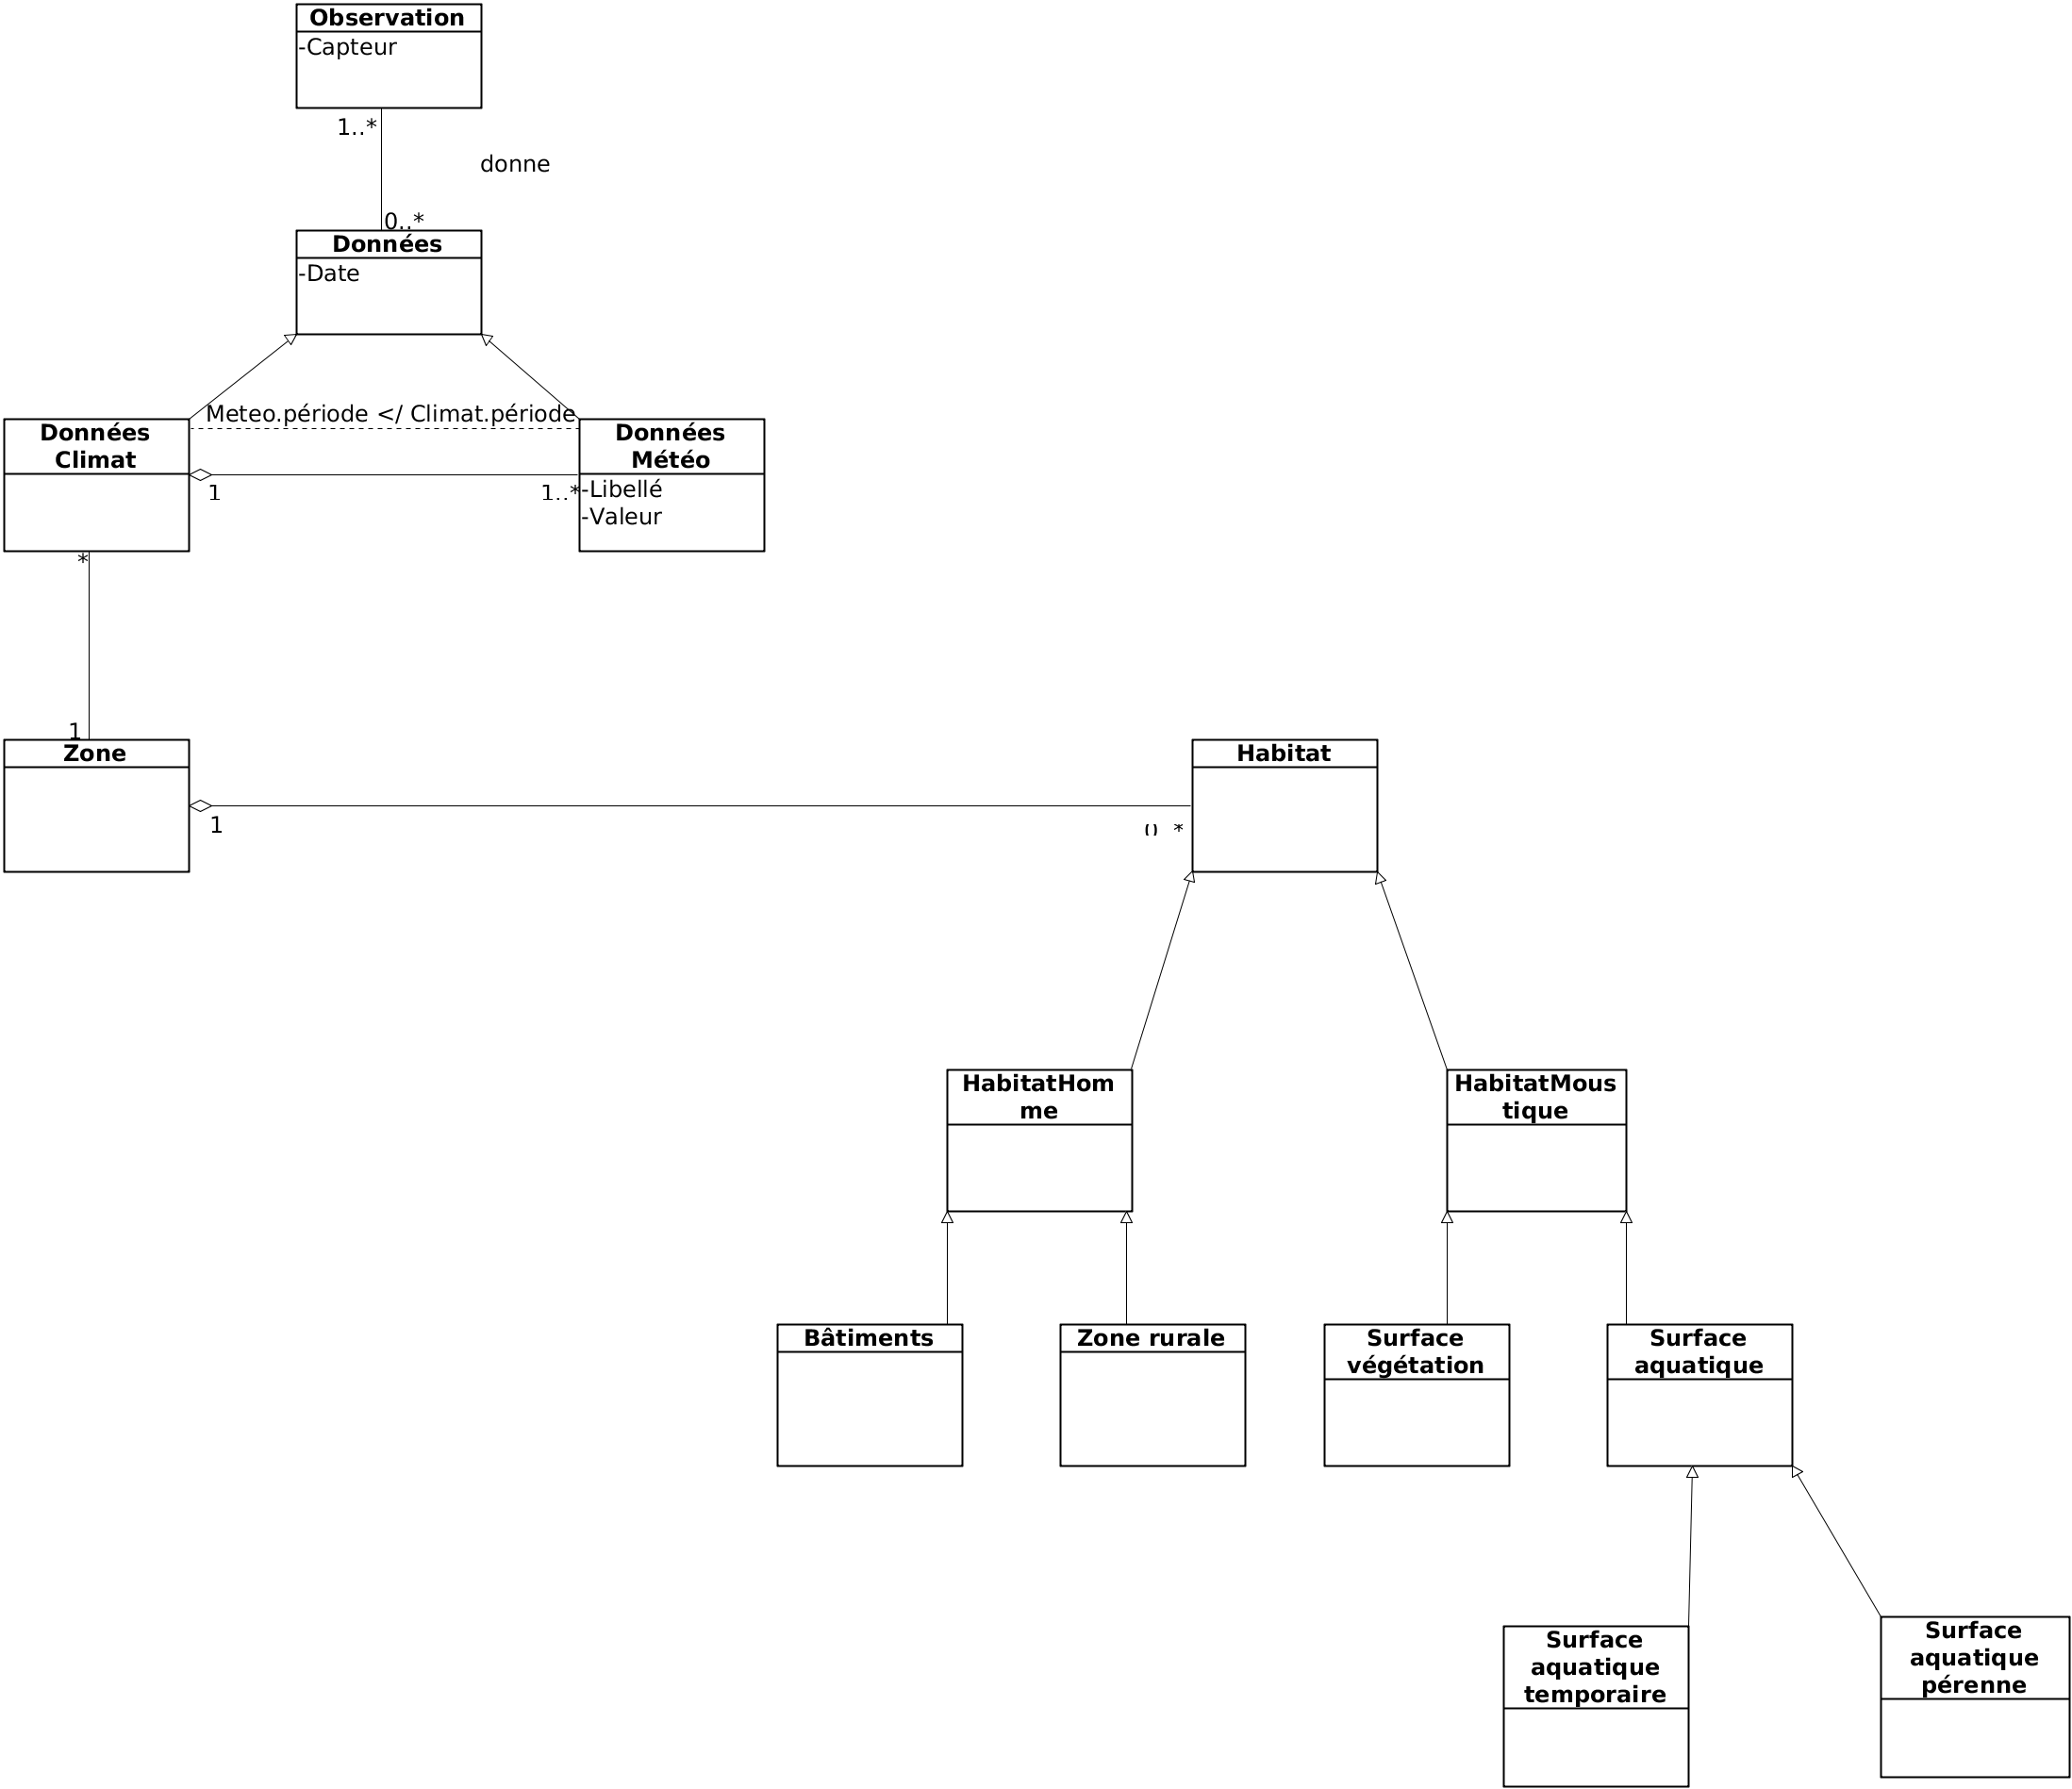
\includegraphics[width=14cm]{DiagrammeUMLsimplif.png}\\
\caption{\label{UMLSimplif_malaria} Modèle UML simplifié des indicateurs du paludisme}
\end{figure}
\end{center}

Le modèle conceptuel simplifié comprend les catégories de risques suivantes : \\
\begin{itemize}
\item Données climatologiques (précipitations, température etc). => aléa
\item Présence de surface d'eau (temporaires ou pérennes) => aléa
\item Présence de surface végétales => aléa
\item Habitations humaines => vulnérabilité\\
\end{itemize}

La présence humaine est indispensable pour qu'il y ait un risque (vulnérabilité) dans une zone. La présence de bâtiments a été retenue comme facteur de risque lié à cette présence humaine. Les surfaces végétales et les surfaces d'eau sont retenues respectivement  comme lieu d'habitation potentiel pour les moustiques anophèles et pour les larves de moustiques anophèles.

Ce modèle UML simplifié nous a servi de base pour conceptualiser le raisonnement de construction des indicateurs et la définition des traitements.

%Introduire le fait que les observations (terrain / satelite) ont été faites sur le territoire concerné, qu'elles concernent le moustique, l'habitat humain et la végétation/surface aquatique, éventuellement les données climatiques. Ces observatiosn vont être le point de départ de la chaîen de traitments à effectuer. 

%\subsection{Indicateurs}

\section{Raisonnement}

A partir des données disponibles, du modèle conceptuel simplifié et en collaboration avec des experts dans le domaine de l'environnement-santé et de la télédétection le raisonnement nous a permis de définir les traitements nécessaires pour l'élaboration de cartes de risque du paludisme. Nous nous sommes basés sur les travaux réalisés par Nadine Dessay. Une fois les traitements nécessaires définis nous nous sommes intéressés à la conceptualisation de l'enchaînement des traitements et des données. Cette partie est indispensable pour comprendre le futur fonctionnement de la chaîne de traitements.\\

\newpage

De façon très schématique le fonctionnement de la chaîne de traitements correspond au modèle suivant:\\


\begin{center}
\begin{figure}[h] \centering
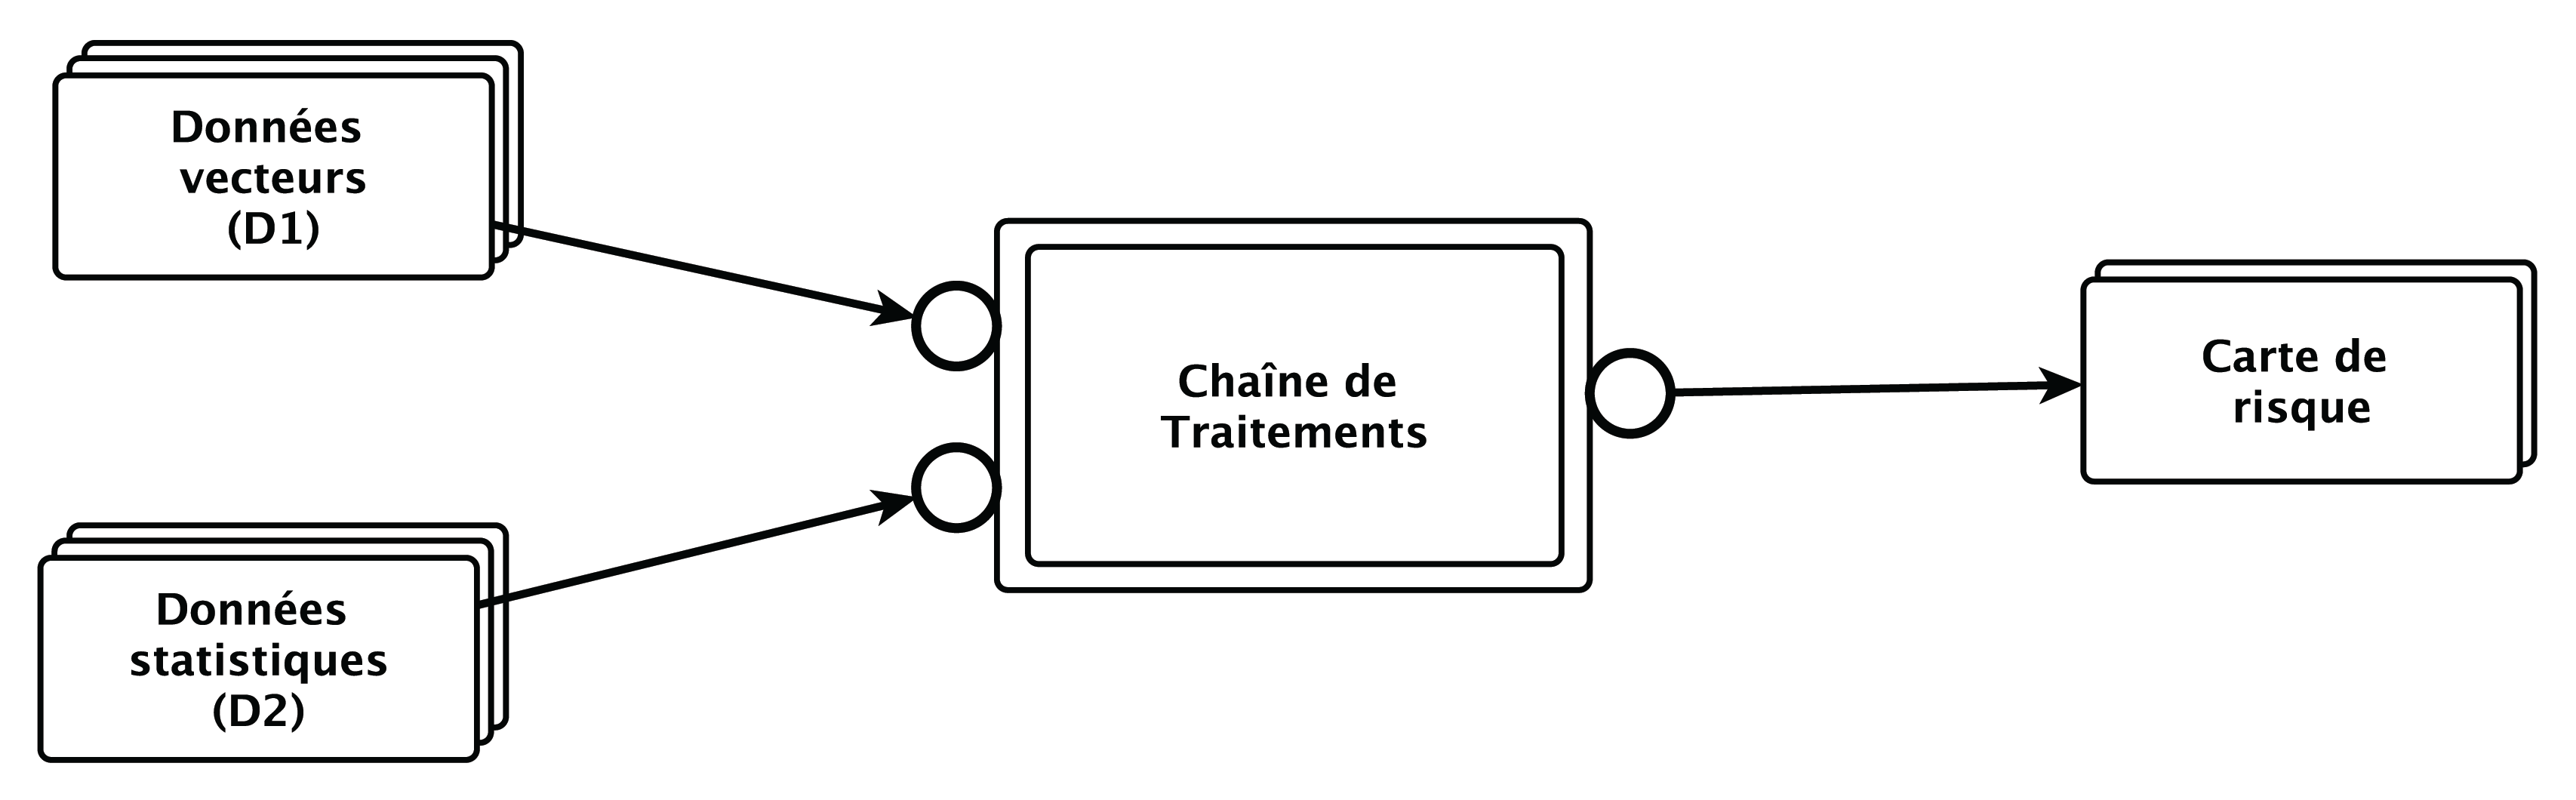
\includegraphics[width=12cm]{Traitement1.png}\\
\caption{\label{Traitements1} Description générale de la chaîne de la chaîne de traitements}
\end{figure}
\end{center}

Des traitements sont effectués sur des données de format vecteur et sur des données statistiques pour obtenir en sortie une carte de risque.
Nous expliquons dans un premier temps ce que fait un traitement et comment fonctionne une donnée. Ceci est fait à partir de \textbf{diagrammes de classes}.\\
Par la suite, des catégories de données et des catégories de traitements de la chaîne sont proposées à l'aide de \textbf{modèles conceptuels des hiérarchies}. Ceci permet de mieux comprendre le fonctionnement et les différentes étapes de la chaîne de traitements.\\


\subsection{Description des données et des traitements}

Nous allons décrire et expliquer les traitements réalisés au sein de la chaîne. Cette description peut être regroupée en 2 parties: \\

\begin{itemize}
\item La description globale de ce que fait un traitement
\item La description des données\\
\end{itemize}

Dans la suite de cette partie, nous expliquons successivement les deux aspects cités ci-dessus. Le modèle (\ref{TraitementModele}) qui suit décrit le fonctionnement d'un traitement.



\paragraph{1) Description globale de ce que fait un traitement\\}

Un traitement correspond à un propriétaire (contact), celui qui a respectivement développé ou défini le traitement. Chaque traitement correspond également à une ou plusieurs fonctionnalités et à une catégorie de traitements. Un traitement informatique comme par exemple l'édition nécessite les fonctionnalités comme par exemple ouvrir un fichier ou exporter un fichier. Un traitement correspond à diverses catégories de traitement qui pour nous ont été déterminées et nommées : pré-traitements, traitements et post-traitements. (cf. \citep{Lin2011})\\

Un traitement met en jeu trois types de données : des données d'entrée, des données de sortie et des données de paramétrage. Les données seront expliquées plus en détail dans le paragraphe (\ref{descrDonnes}) suivant.\\

Exemple d'un traitement: \textbf{shp2pgsql\\}
\begin{itemize}

\item Propriétaire: PostGIS / GDAL
\item Fonctionnalité(s): Transformation du format, Reprojection
\item Catégorie: Traitement
\item Donnée d'entrée: Fichier au format vecteur (shape)
\item Donnée en sortie: Fichier au format ".sql"
\item Donnée de paramétrage: postgis.sql, spatial\_ref.sql

\end{itemize}

\begin{figure}[H] 
\begin{center}
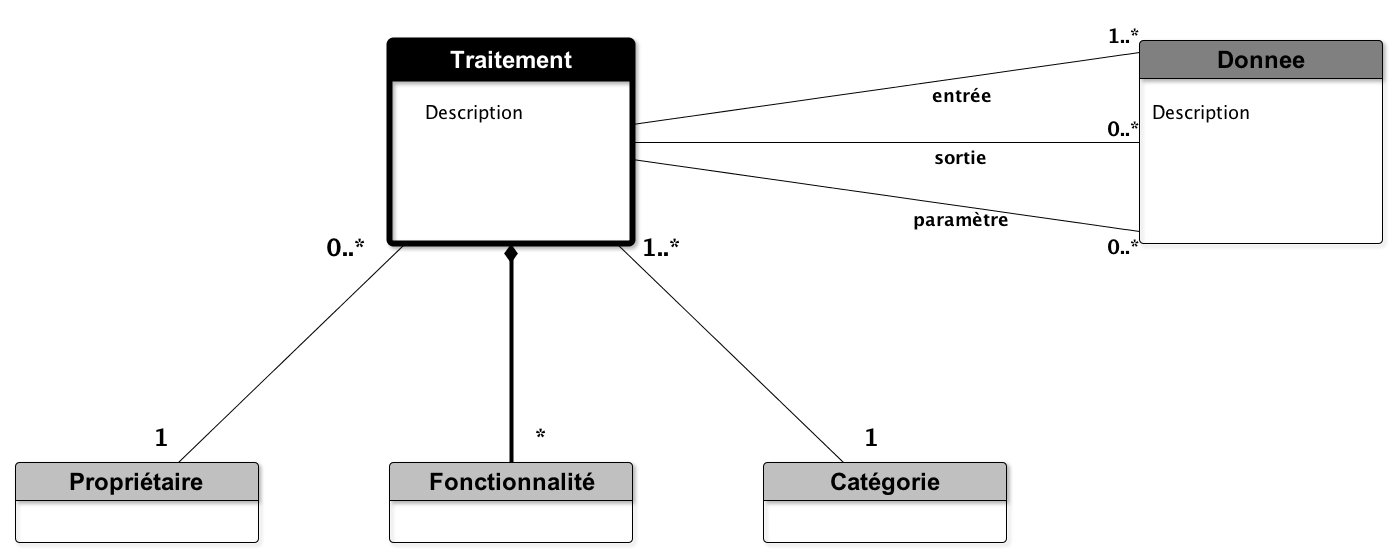
\includegraphics[width=15cm]{DescriptionTraitement5712.png}\\
\caption{\label{TraitementModele} Description du fonctionnement d'un traitement}
\end{center}
\end{figure}

\newpage
\paragraph{2) Description des données\\} \label{descrDonnes}

Décrire les traitements d'un système demande également de décrire les données utilisées. Une données correspond à une catégories de données, un  propriétaire et un format. (cf. \citep{ElKader2006}) \\

\begin{figure}[H] 
\begin{center}
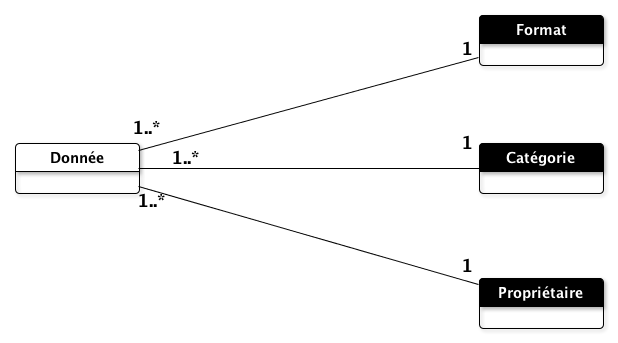
\includegraphics[width=9cm]{DescriptionDonnees}\\
\caption{\label{DescriptionDonnees} Description des données }
\end{center}
\end{figure}

Dans le contexte de ce travail, les formats de données utilisés sont les suivants : Format vecteur (fichiers de forme géoréférencés), format raster (images composites géoréférencés) et format tableur (statistiques). Ces données correspondent à des fonctionnalités comme par exemple la création de zones tampons. Chaque donnée est également caractérisée par un propriétaire (contact) et une catégorie de données. Nous pouvons regrouper les données utilisées, dans notre contexte, en deux catégories principales : les données issues de capteurs satellites et les données récoltées sur le sol (stations ou capteurs au sol).\\ 
%Une donnée correspond également à un type de données. Une donnée vecteur peut être par exemple de "type" ligne ou polygone. \\


Exemple de donnée: \textbf{b\_bati.shp}\\
\begin{itemize}

\item Propriétaire: Nadine Dessay
\item Catégorie: Raster
\item Format: vecteur (shape)

\end{itemize}

\newpage

\subsection{Les catégories de données et de traitements} \label{catdonnees}

\subsubsection{Les catégories de données}
Le modèle conceptuel des catégories de données (\ref{ModeleDonneesMin}) décrit de façon formelle les catégories de données qui sont utilisées par la chaîne de traitements.\\

\begin{figure}[H]
\begin{center}
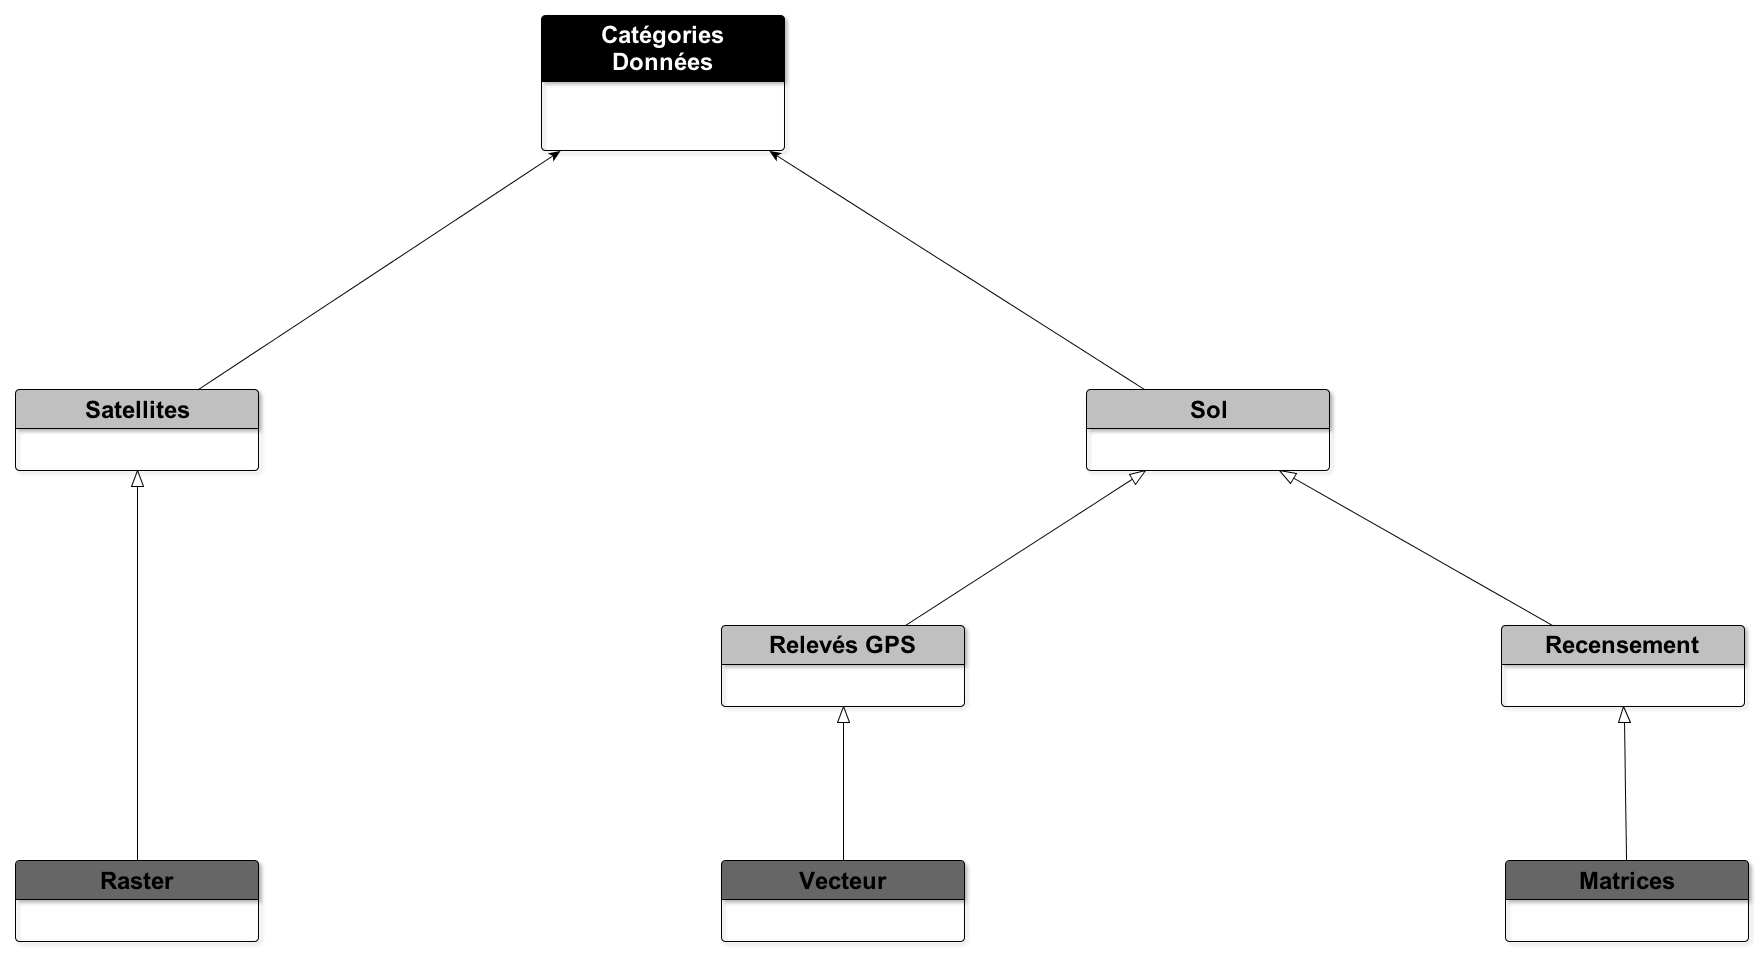
\includegraphics[width=16cm]{ModeleDonneesMin}\\
\caption{\label{ModeleDonneesMin} Modèle conceptuel des catégories de données de la chaîne de traitements}
\end{center}
\end{figure}


Les données de la chaîne de traitements sont issues de sources diverses. Les \textbf{données issues de satellites} correspondent aux données obtenues à partir de satellites (passifs ou actifs).
Les \textbf{données issues du sol} sont les données qui proviennent de capteurs ou de toute autre source se situant sur le sol terrestre. \\

Les satellites produisent des \textbf{images raster}, à partir desquelles, en ayant recours à des traitements de télédétection, peuvent être extraites de nombreuses informations. Pour notre chaîne de traitements, les informations suivantes ont été extraites par des experts en télédétection (Nadine Dessay):\\

\begin{itemize}
\item Eau: Les surfaces d'eau
\item Végétation: Les arbres etc.
\item Urbanisation: Bâtiments\\
\end{itemize}

Les données récoltées sur le \textbf{sol} peuvent correspondre à différentes catégories. Par exemple, une station météo peut fournir des données de catégorie vecteur ou raster. Des relevés GPS fournissent des vecteurs. Des statistiques (catégorie matrices) sont obtenues à partir de recensements de population par exemple.


\subsubsection{Les catégories de traitements}



Nous proposons trois grandes catégories de traitements: Les \textbf{pré-traitements}, les \textbf{traitements} et les \textbf{post-traitements}.
La catégorie des pré-traitements recouvre l'ensemble des opérations qui préparent les données pour qu'elles puissent être traitées. Dans le cadre de ce travail il est nécessaire de stocker les données et d'effectuer des requêtes SQL afin de sélectionner les données à en fonction des traitements.\\

La catégorie des traitements recouvre les traitements proprement dits, c'est à dire les traitements qui vont créer ou modifier des données. Cette catégorie présente trois sous-catégories : les traitements \textbf{statistiques} ,les traitements \textbf{d'analyse spatiale} et les traitements de \textbf{transformation}. \\

Les traitements statistiques concernent les calculs de densités de population, de densité de points et le calcul de la taille de cellule des couches raster.

Les traitements d'analyse spatiale sont les traitements géographiques sur les \textbf{fichiers de forme} (shape) (par exemple intersection entre deux fichiers de forme vecteurs).\\

Les traitements de transformation correspondent aux traitements qui modifient le format des données. Par exemple, pour insérer un fichier vecteur dans une base de données spatiale, il est nécessaire d'effectuer une transformation vers le format ".sql".

Les post-traitements concernent tout ce qui est représentation des résultats obtenus, par exemple une reclassification d'une image raster pour faire ressortir une information plus clairement.



\begin{figure}[H]
\begin{center}
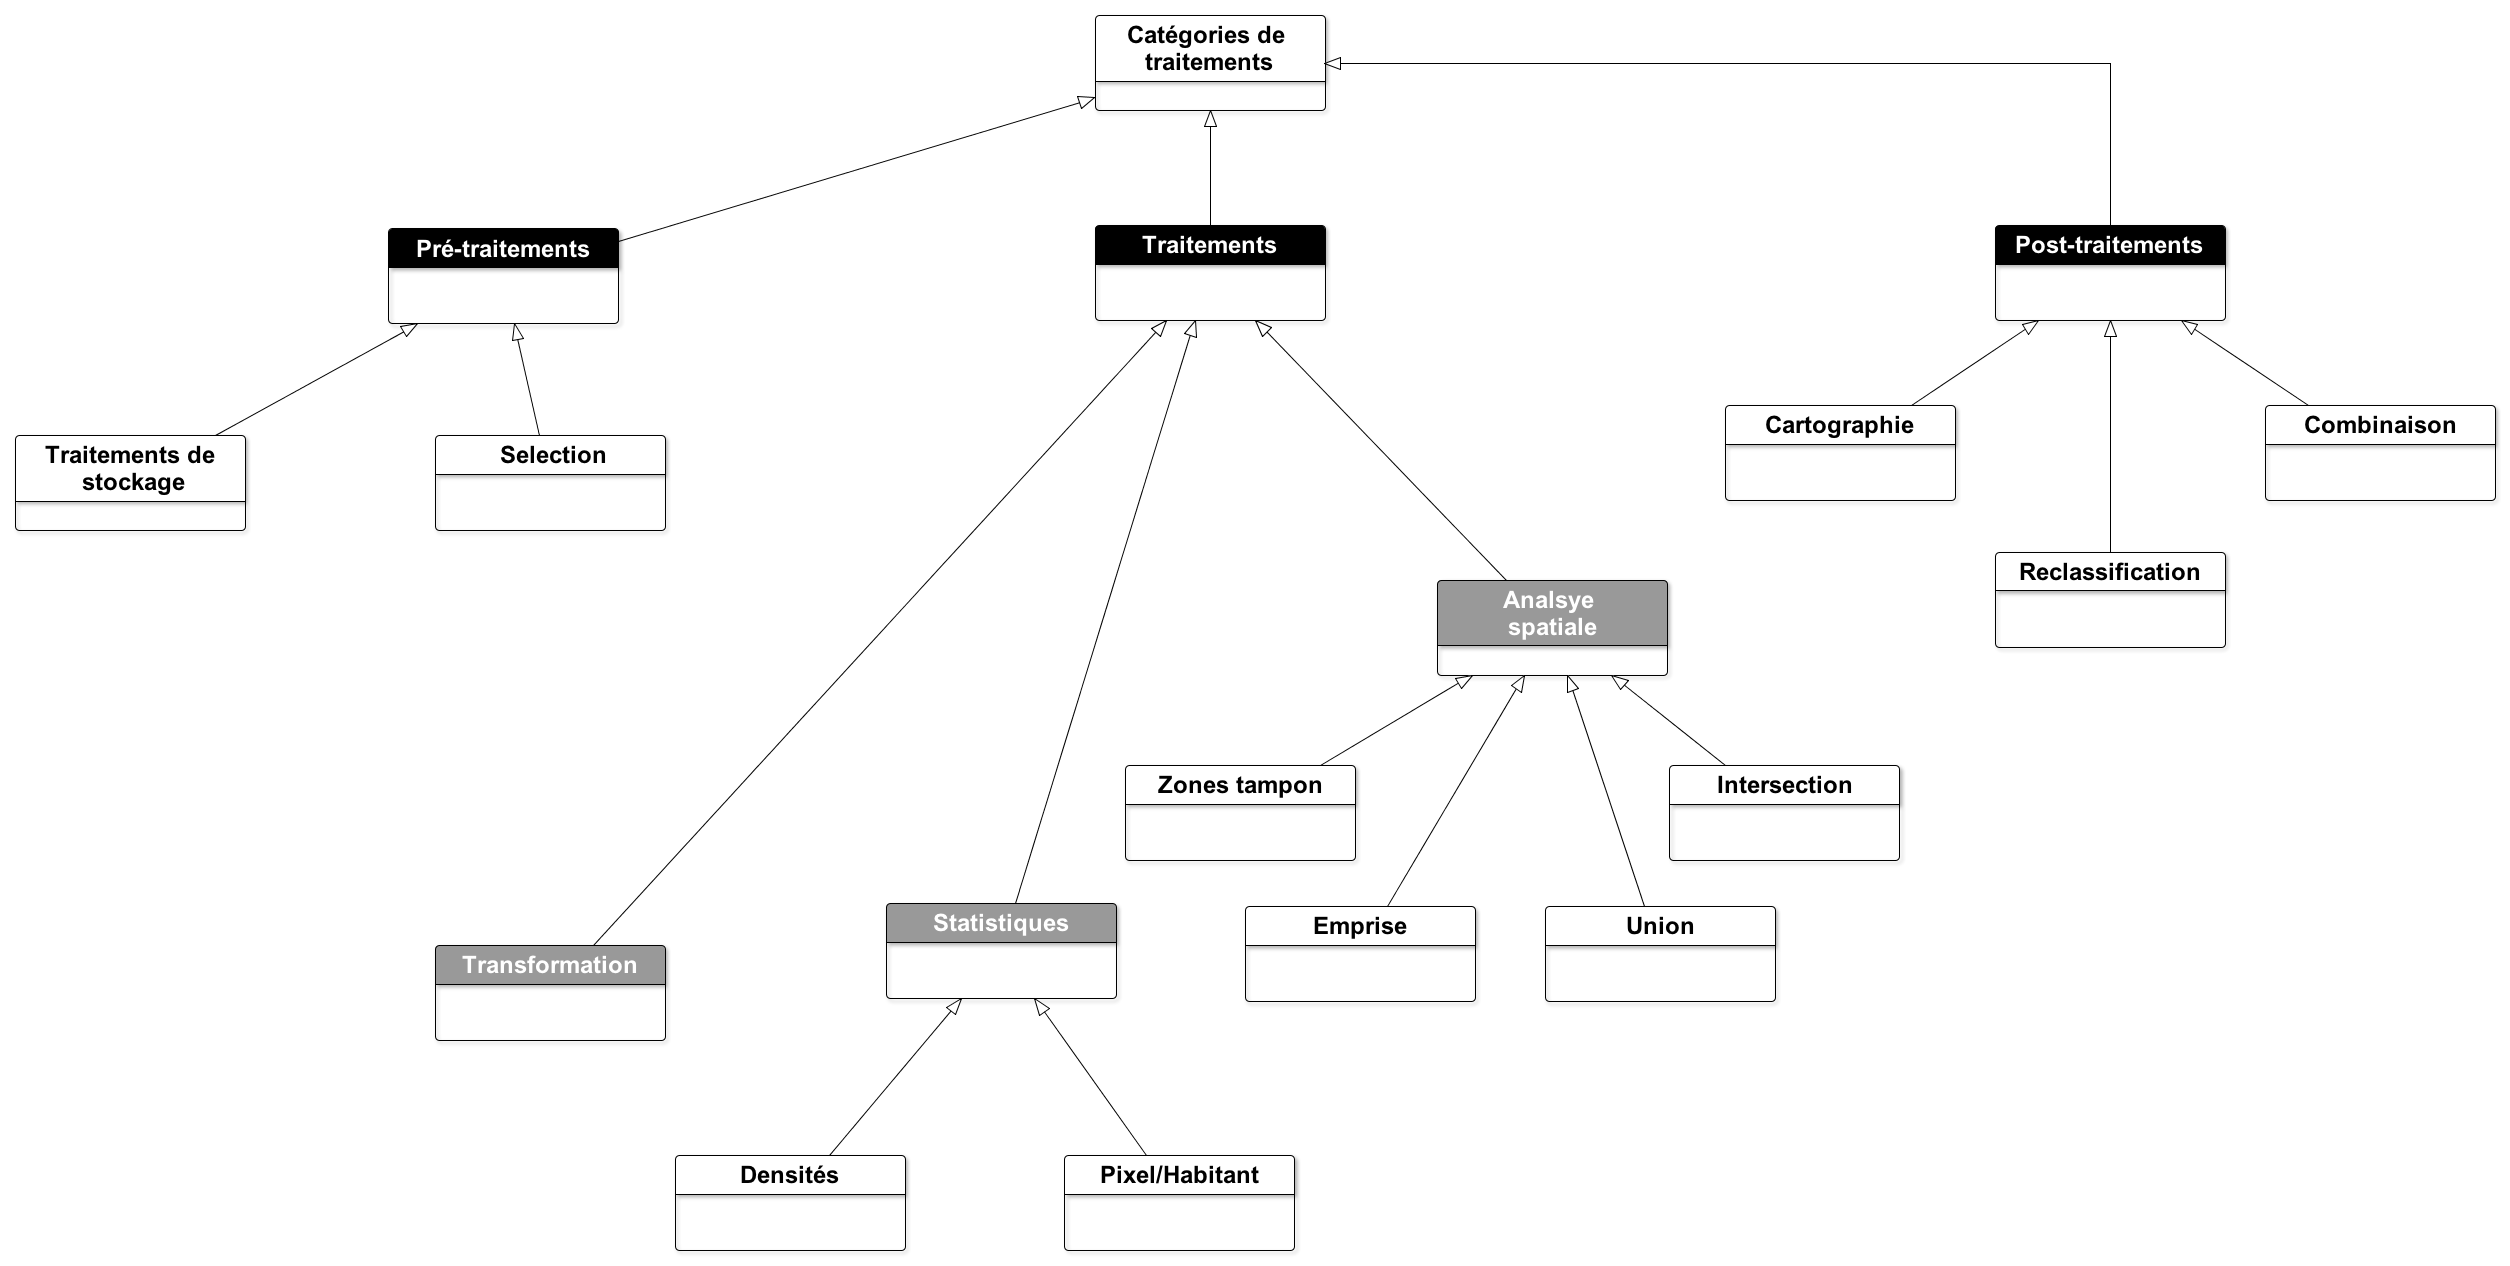
\includegraphics[width=16cm]{ModeleTraitements2}\\
\caption{\label{ModeleTraitements} Modèle conceptuel des hiérarchies de catégories de traitements de la chaîne de traitements}
\end{center}
\end{figure}



\subsection{Conceptualisation de la chaîne de traitements}

Le modèle conceptuel des traitements permet de représenter la dynamique de la chaîne de traitements, c'est-à-dire les opérations et traitements qui sont réalisées en fonction d'autres événements. 
Ce modèle permet donc de représenter et d'expliquer de façon conceptuelle le fonctionnement du système sans faire référence aux choix qui ont été réalisés (par exemple quelle librairie a été utilisée, quel langage informatique etc.). Le modèle explique donc les traitements qui sont effectués dans la chaîne mais il n'explique pas comment ils sont effectués.  \\

Pour illustrer les différentes opérations de la chaîne de traitements, nous allons détailler successivement comment se construit la chaîne de traitements à partir des descriptions précédentes et comment l'instanciation est réalisable à partir du modèle de départ (cf \ref{Traitement11})\\

%Pour faciliter la représentation des chaînes abstraites nous utiliserons le langage graphique proposé par Yuan Lin (\ref{LinGraph}). Les ports de données associés à un traitement abstrait ont pour objectif de distinguer les différents flux de données en terme d’entrée / sorties \citep{Lin2011}.



\subsubsection{Description générale}

Pour créer une carte de risque, il est nécessaire d'effectuer des traitements sur des données. Les données d'entrée correspondent à deux formats différents : format vecteur et format statistique. Ces données sont utilisées par la chaîne de traitements pour effectuer les traitements nécessaires pour cartographier le risque.\\


\begin{figure}[H]
\begin{center}
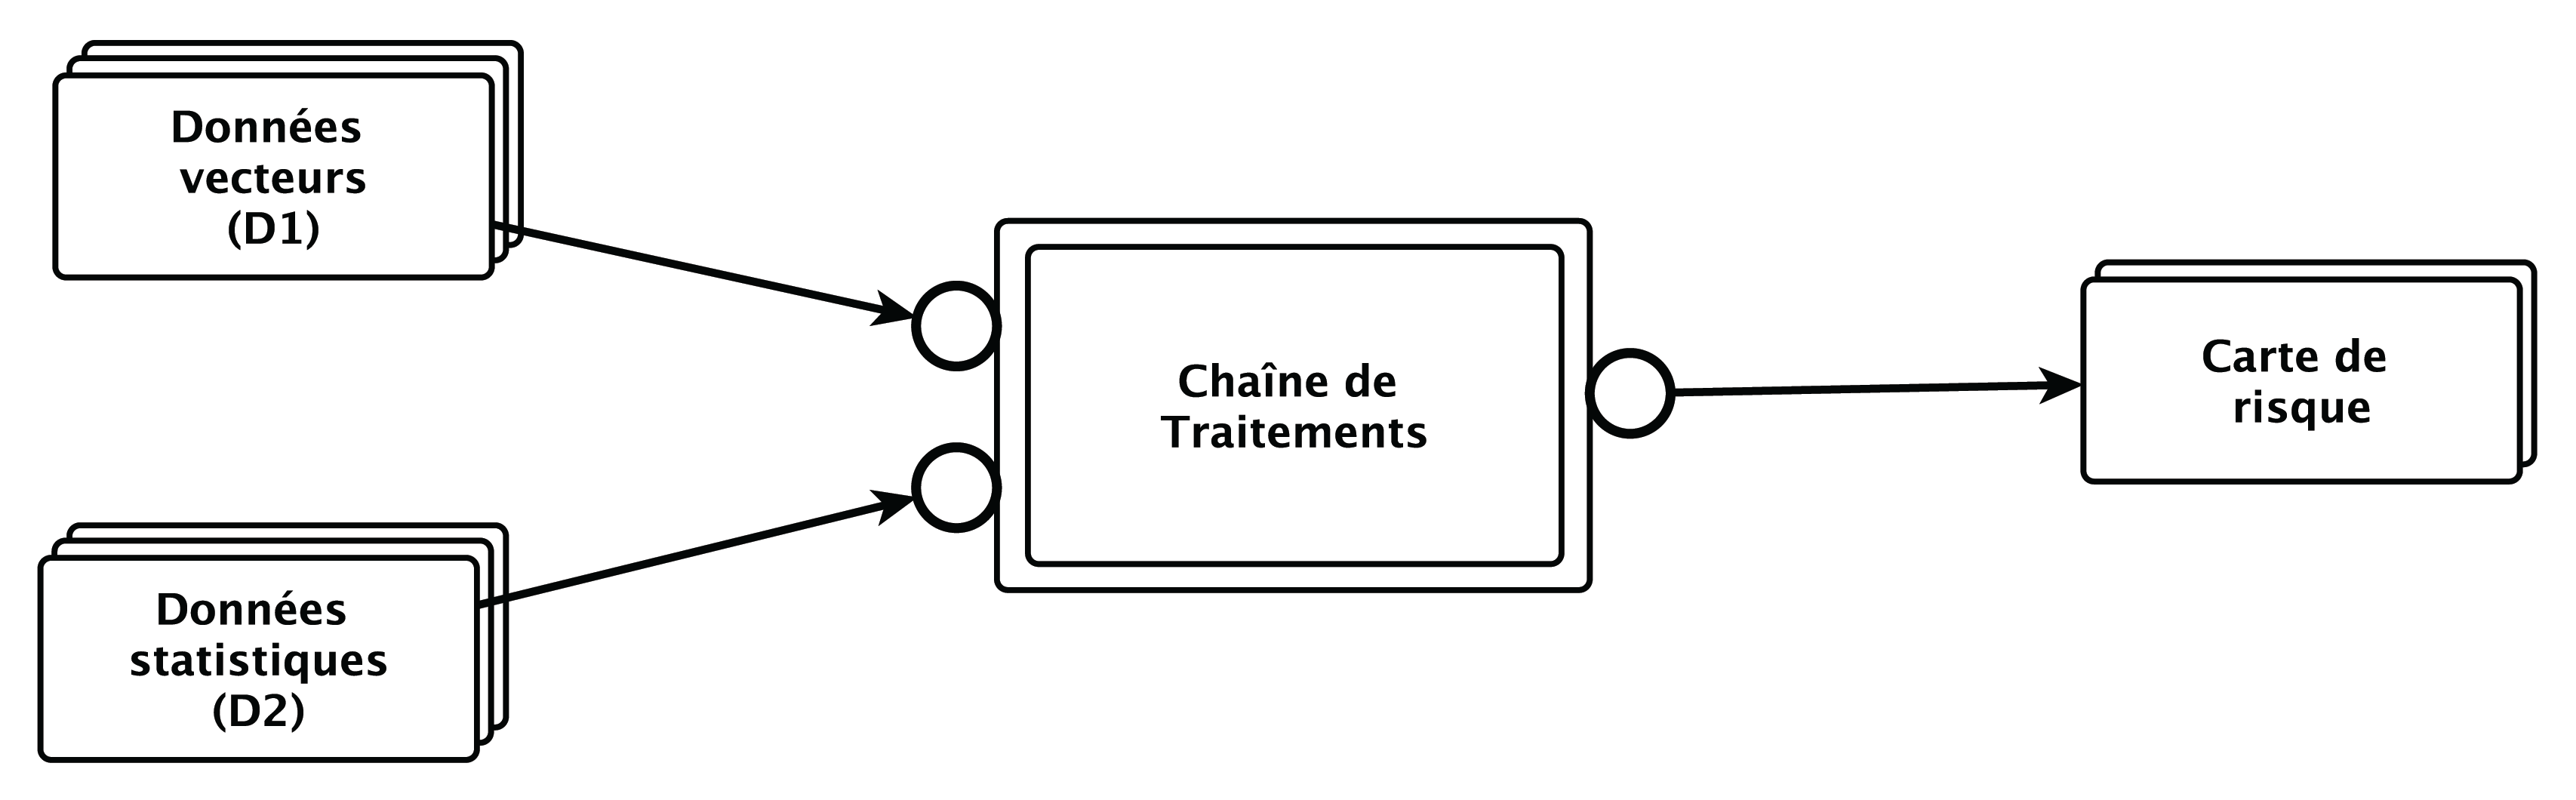
\includegraphics[]{Traitement1.png}\\
\caption{\label{Traitement11} Description générale}

\end{center}
\end{figure}




\subsubsection{Chaîne abstraite}

Dans un premier temps, les données vecteurs sont stockées (traitements de stockage) dans une base de données. Par la suite, des \textbf{sélections} permettent de définir précisément les données qui seront traitées lors de chaque traitement.\\

Le risque est la combinaison entre \textbf{l'aléa} et la \textbf{ vulnérabilité}. Deux grandes catégories de traitements sont effectuées : les traitements de vulnérabilité et les traitements d'aléa. Le traitement de risque permet de créer des cartes de risque.\\


\begin{figure}[H]
\begin{center}

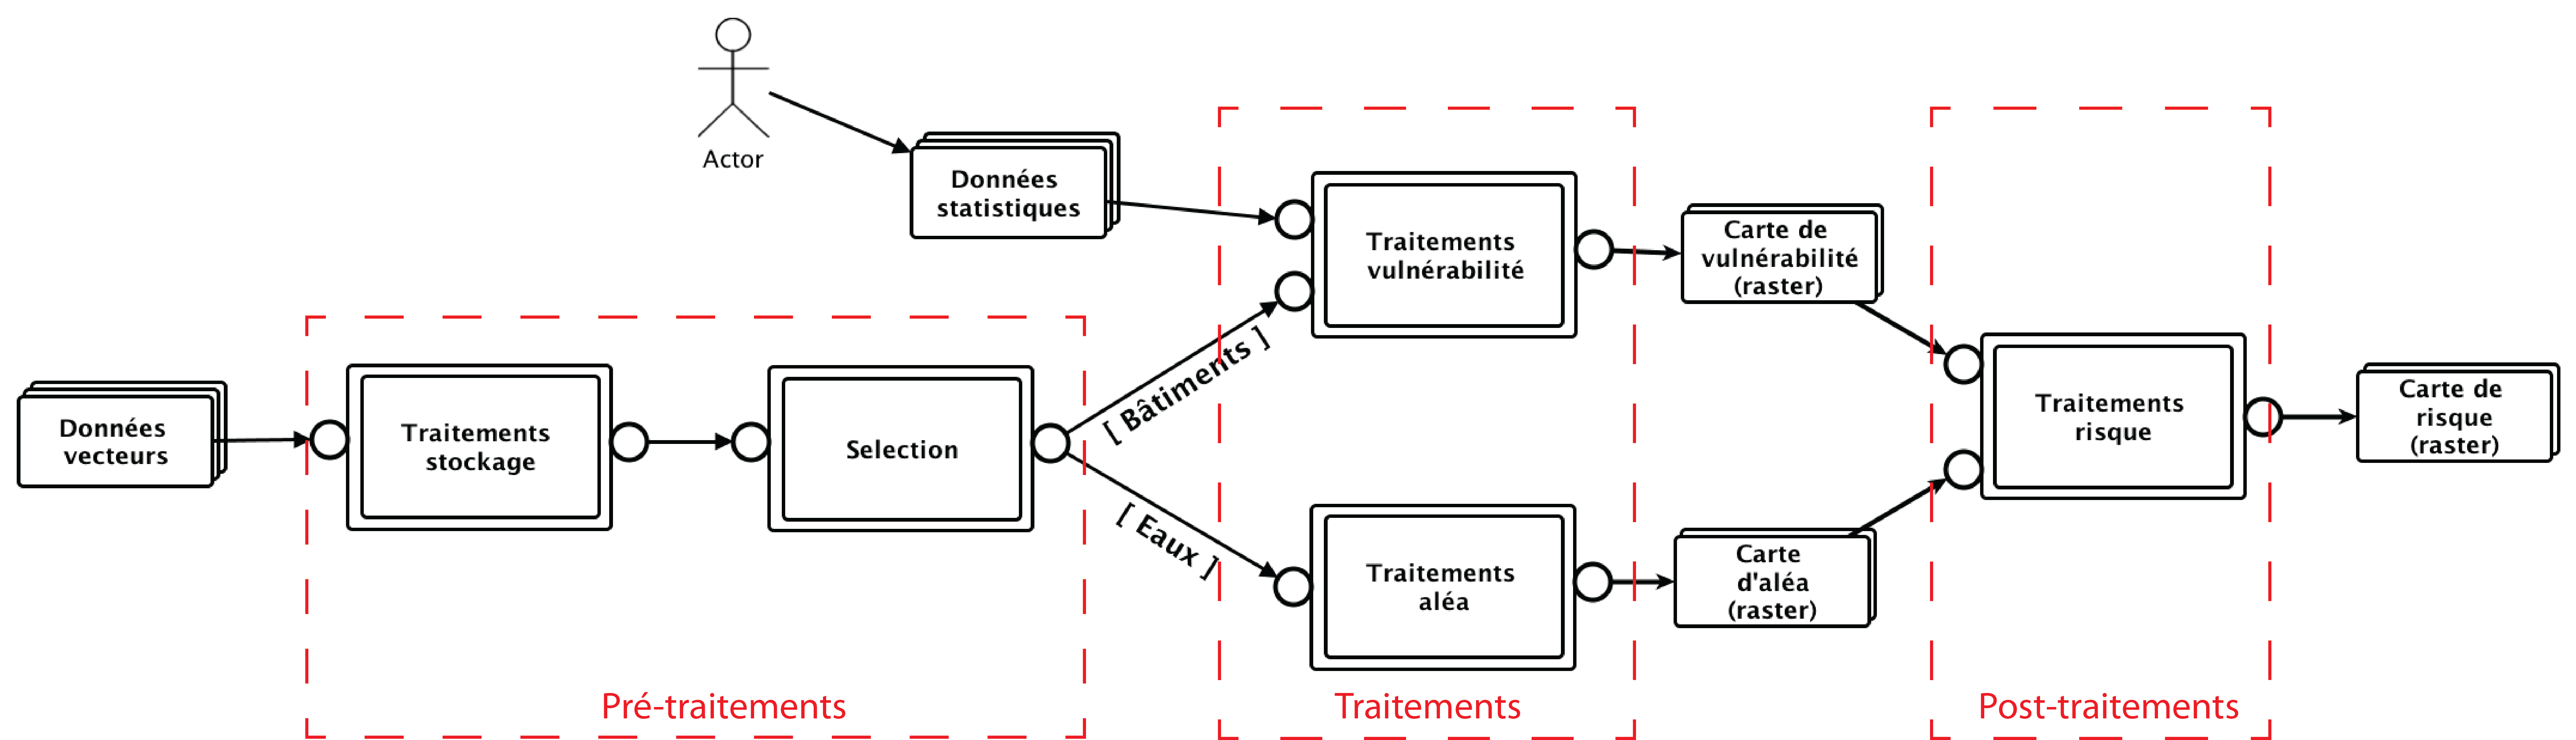
\includegraphics[width=15cm]{traitements2.png}\\
\caption{\label{Traitement12} Chaîne abstraite}
\end{center}
\end{figure}



\subsubsection{Traitements élémentaires de la chaîne de traitements}

Chaque donnée vectorielle stockée dans la base de données est dans un premier temps reprojetée (la projection de la base de données spatiale et de toutes les données insérées sera la même). Les données sont insérées dans une base de données spatiale (créée dans un \textbf{SGBD} au cours de l'exécution de la chaîne de traitements). Des requêtes SQL permettent de sélectionner (filtrer) les données à utiliser pour chaque traitement.\\

Les traitements de vulnérabilité correspondent à deux catégories de traitements : des traitements d'analyse spatiale et des traitements statistiques. La chaîne de traitements demande à l'utilisateur le nombre d'habitants de la zone d'études (= données statistiques). La chaîne de traitements crée une carte de vulnérabilité en combinant les deux catégories de traitement.\\

Les traitements d'aléa correspond à des traitements d'analyse spatiale sur les données "eau" (format vecteur). L'ensemble de ces traitements permettent de créer une carte d'aléa.\\

Les traitements de risque correspondent à la combinaison de la carte de vulnérabilité et de la carte d'aléa. La carte de risque est le résultat de l'ensemble des traitements.


\begin{figure}[H]
\begin{center}

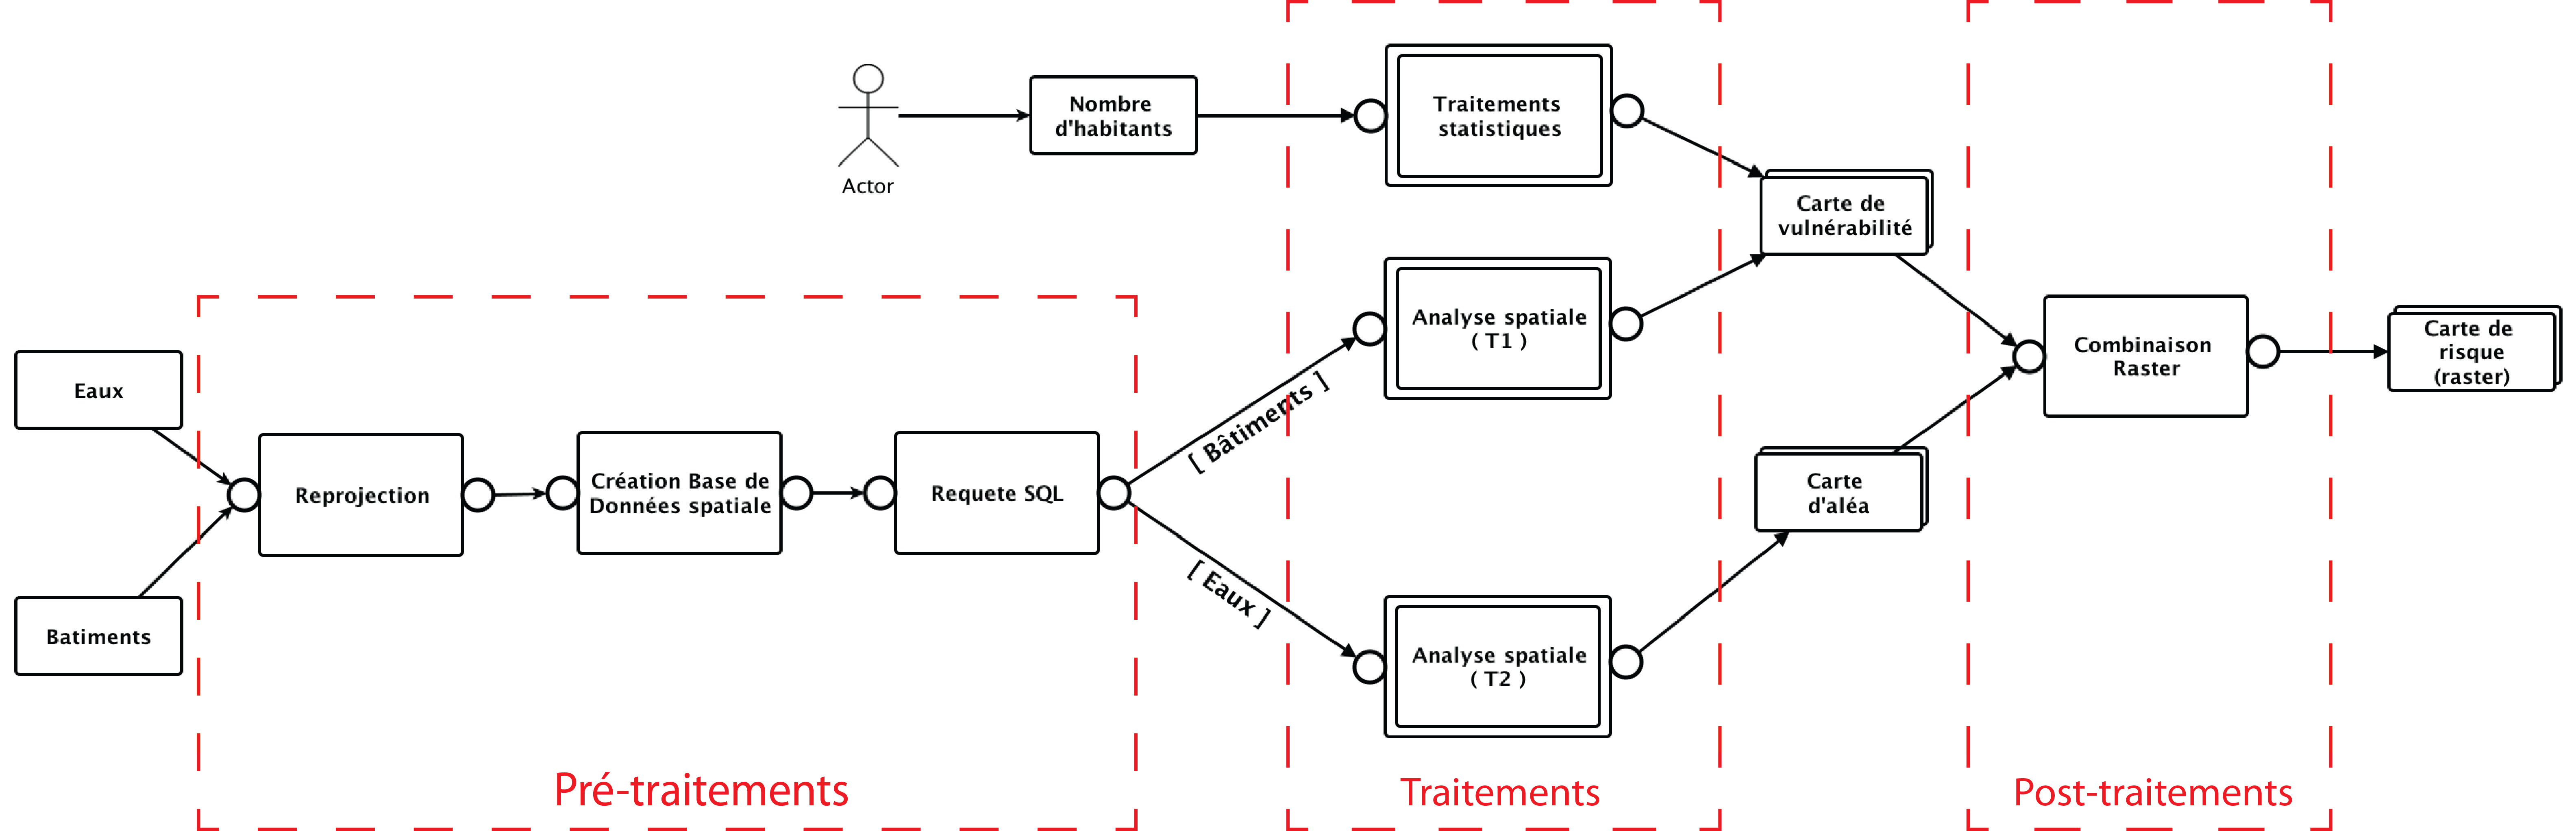
\includegraphics[width=15cm]{Traitements3.png}\\
\caption{\label{Traitement13} Chaine abstraire avec traitements élémentaires}
\end{center}

\end{figure}




\subsubsection{Chaîne de traitements de plus en plus détaillées}

Des requêtes SQL permettent de calculer la surface totale de la couche "bâtiments". A partir des informations saisies par l'utilisateur (nombre d'habitants), la chaîne calcule la densité de population de la zone d'étude. A partir de ces informations, la surface qu'occupe en théorie un habitant permet de calculer la taille théorique d'une cellule pour un habitant. La couche "bâtiments" est ensuite \textbf{rastérisée} en fonction de la taille de la cellule calculée par avant. Pour chaque \textbf{cellule de ce raster}, un point est créé et le calcul de la densité des points permet de créer une carte de vulnérabilité.\\

En ce qui concerne les traitements d'analyse spatiale de l'aléa, plusieurs traitements sont successivement effectués: définition de l'emprise de la zone d'étude, zone tampons autour de la couche "eaux" (400 et 600 mètres), union et intersection des résultats pour arriver à la création d'une carte d'aléa. (cf. Annexes)\\


\begin{figure}[H]
\begin{center}

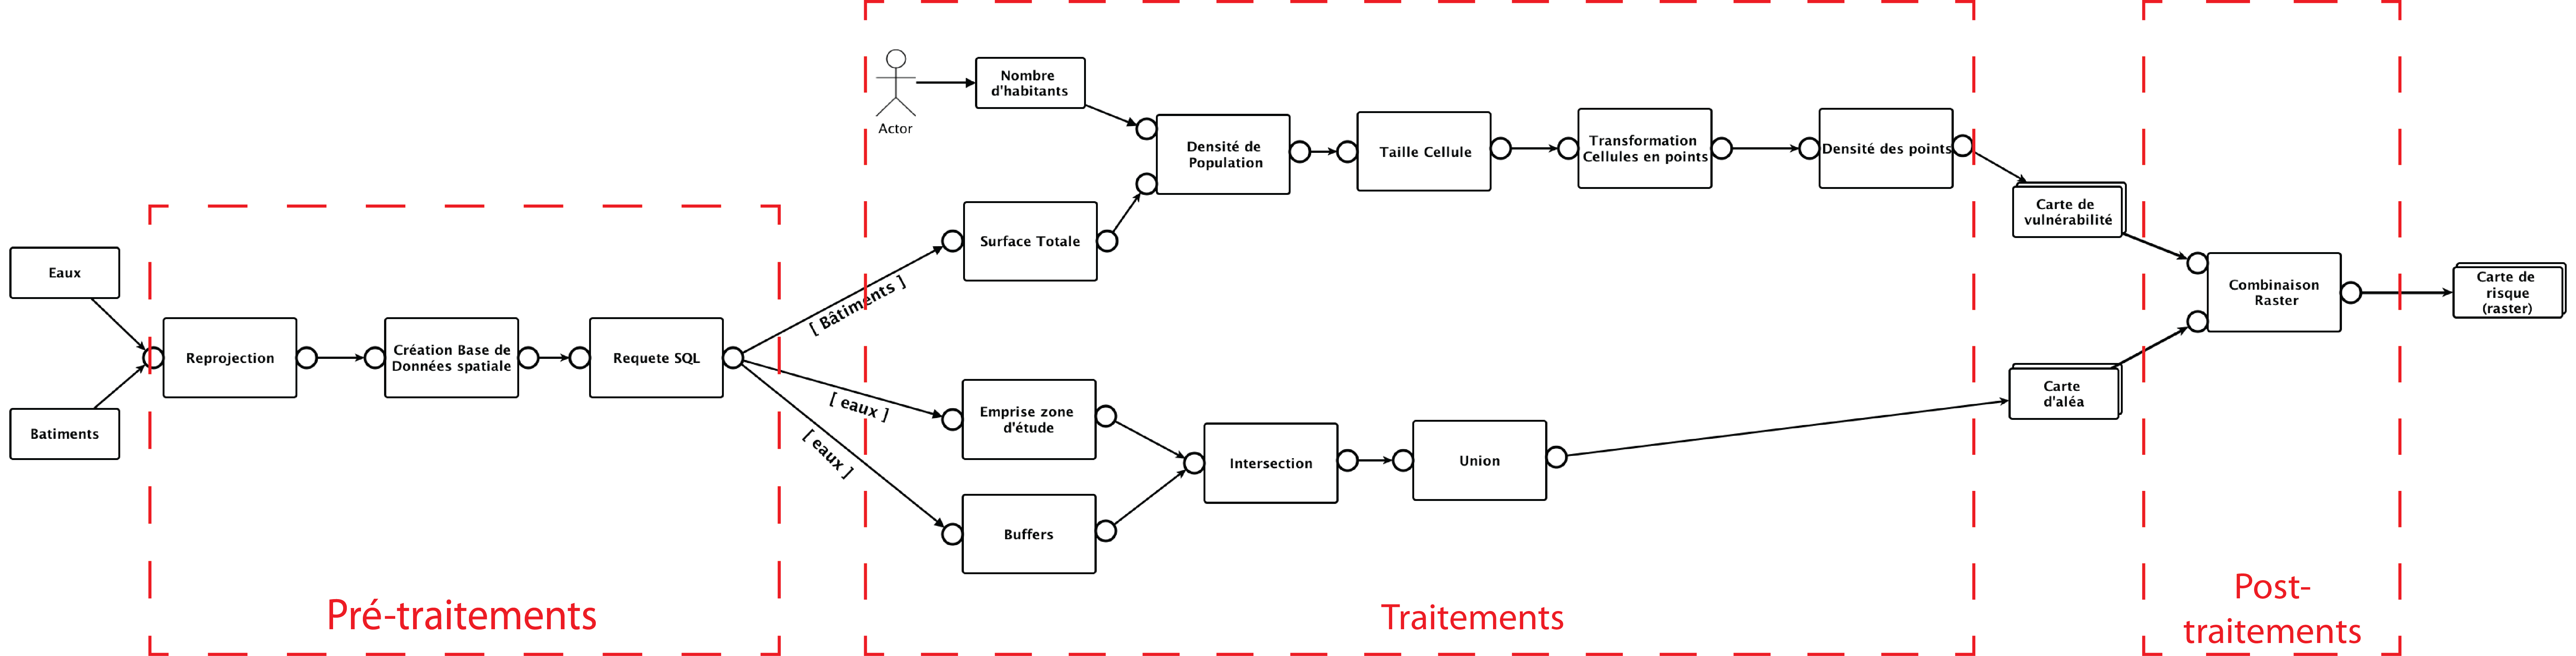
\includegraphics[width=15cm]{Traitement4.png}\\
\caption{\label{Traitement14} Chaîne de traitements de plus en plus détailée}
\end{center}
\end{figure}

\subsubsection{Chaîne de traitements instanciée}


\begin{figure}[H]
\begin{center}

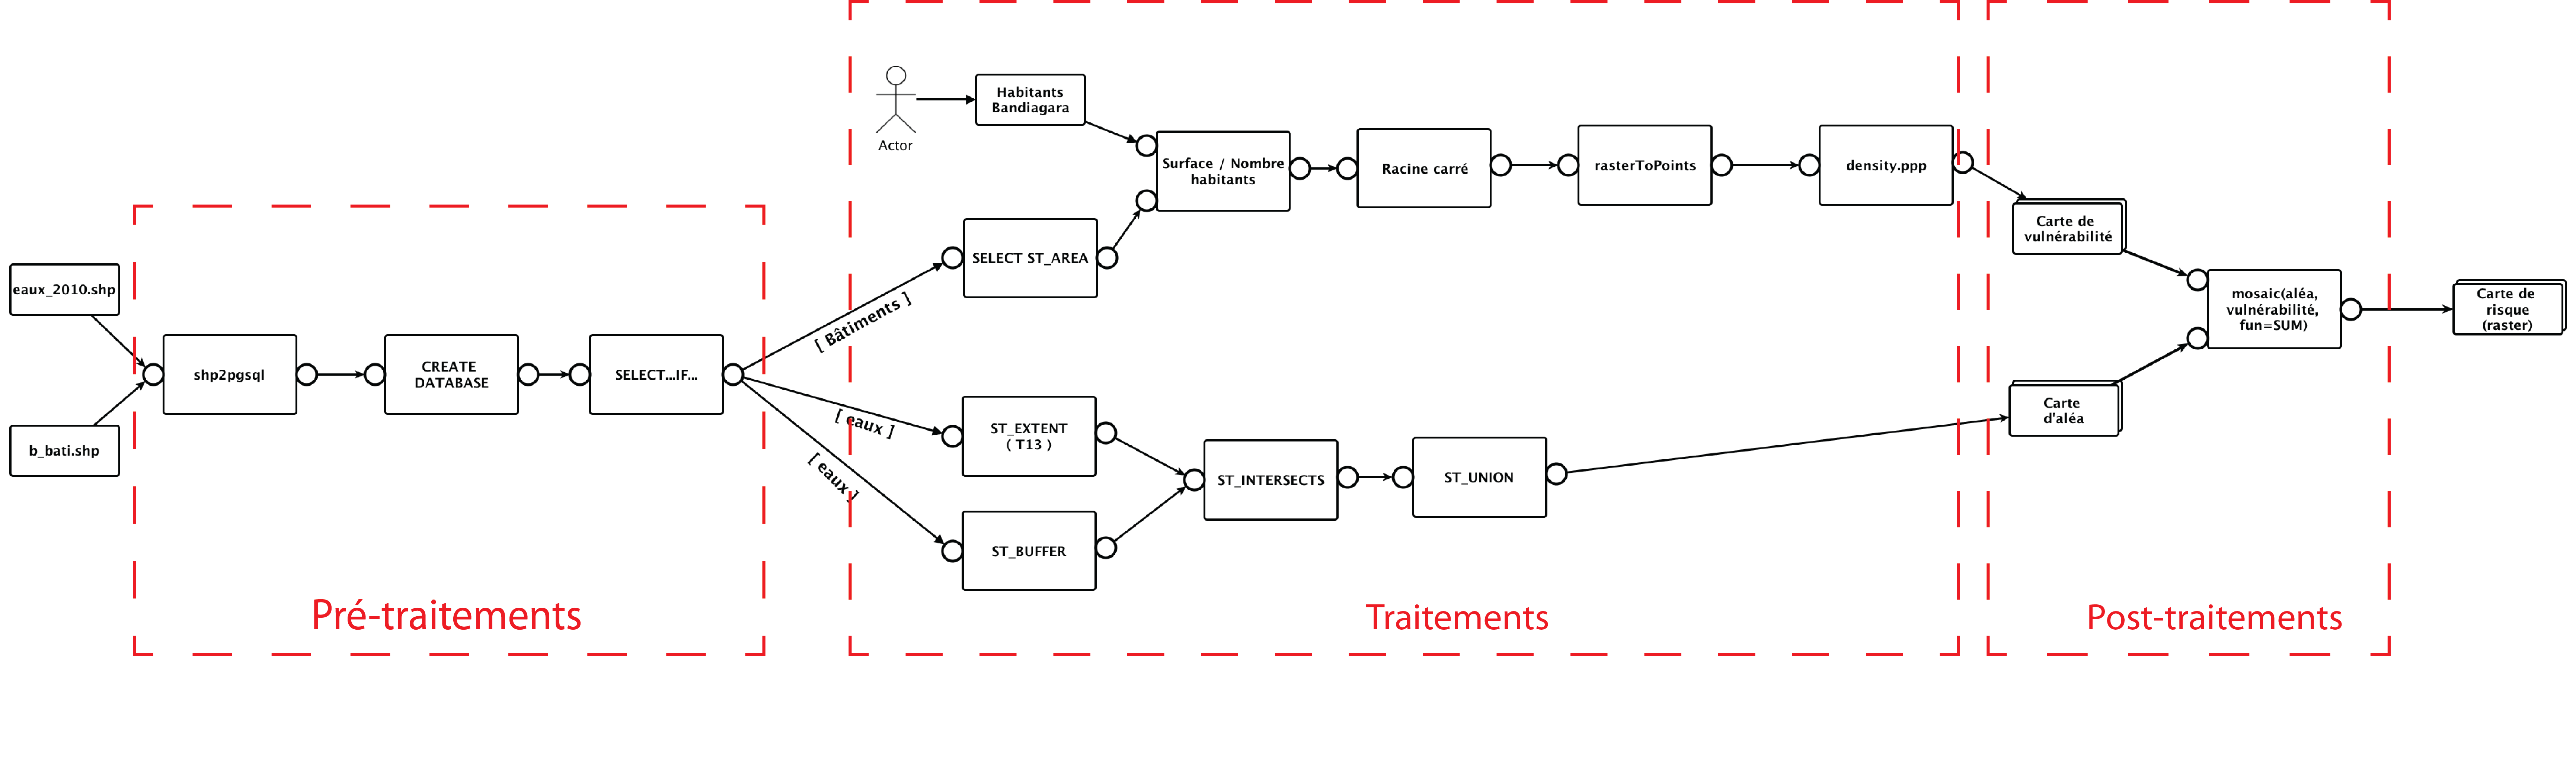
\includegraphics[width=15cm]{chaineinstanc.png}\\
\caption{\label{traitementsInstancie} Chaîne de traitements fermée instanciée}
\end{center}
\end{figure}

Nous utilisons pour l'exécution de la chaîne de traitements fermée deux fichiers de données en entrée: "b\_bati.shp" et "arbres.shp". La fonctionnalité PostGIS "shp2pgsql" permet de transformer et de reprojeter les deux données. Une base de données spatiale est créé et les données sont insérées dans cette base de données. Des requêtes SQL (select...if...) permettent de sélectionner (filtrer) les données nécessaires pour les différents traitements (par exemple "b\_bâti" pour les traitements de vulnérabilité). Les différentes fonctionnalités PostGIS comme "ST\_AREA" (surface d'une couche) ou "ST\_INTERSECTS" (intersection) ainsi que d'autre fonctionnalités R comme par exemple "density.ppp" permettent d'effectuer les traitements souhaités (cf. Annexes). Finalement, la fonctionnalité R "mosaic(...)" permet de combiner la carte de vulnérabilité et la carte d'aléa. 

\section{Conception}

Pour valider sur le plan opérationnel notre approche, nous avons réalisé deux types d'outils. Dans un premier temps, nous avons développé une chaine entièrement automatisée de traitements. L'utilisateur choisit les données d'entrée et la chaîne effectue automatiquement tous les traitements nécessaires pour la création d'une carte de risque. \\

Dans un second temps, nous avons développé un logiciel ouvert, l'utilisateur peut ainsi choisir les traitements qu'il souhaite effectuer.\\

Dans cette partie du travail, nous présentons l'implémentation des deux outils, respectivement l'architecture informatique des deux outils. Les librairies et bibliothèques utilisées sont présentées en Annexe.


\subsection{Architecture informatique de la chaine de traitements et du logiciel ouvert}

Le prototype de la chaîne de traitements et le logiciel ouvert appellent les fonctionnalités des outils PostgreSQL / Postgis (via le JDBC PostgreSQL) et R (via RCaller) via le langage Java. Le schéma suivant explique de façon très simplifiée l'architecture informatique des deux outils. Les deux outils peuvent également se connecter à une bas de données distante. Les autres composants de l'architecture doivent être installés en local sur la machine de l'utilisateur.\\

\begin{figure}[H]
\begin{center}
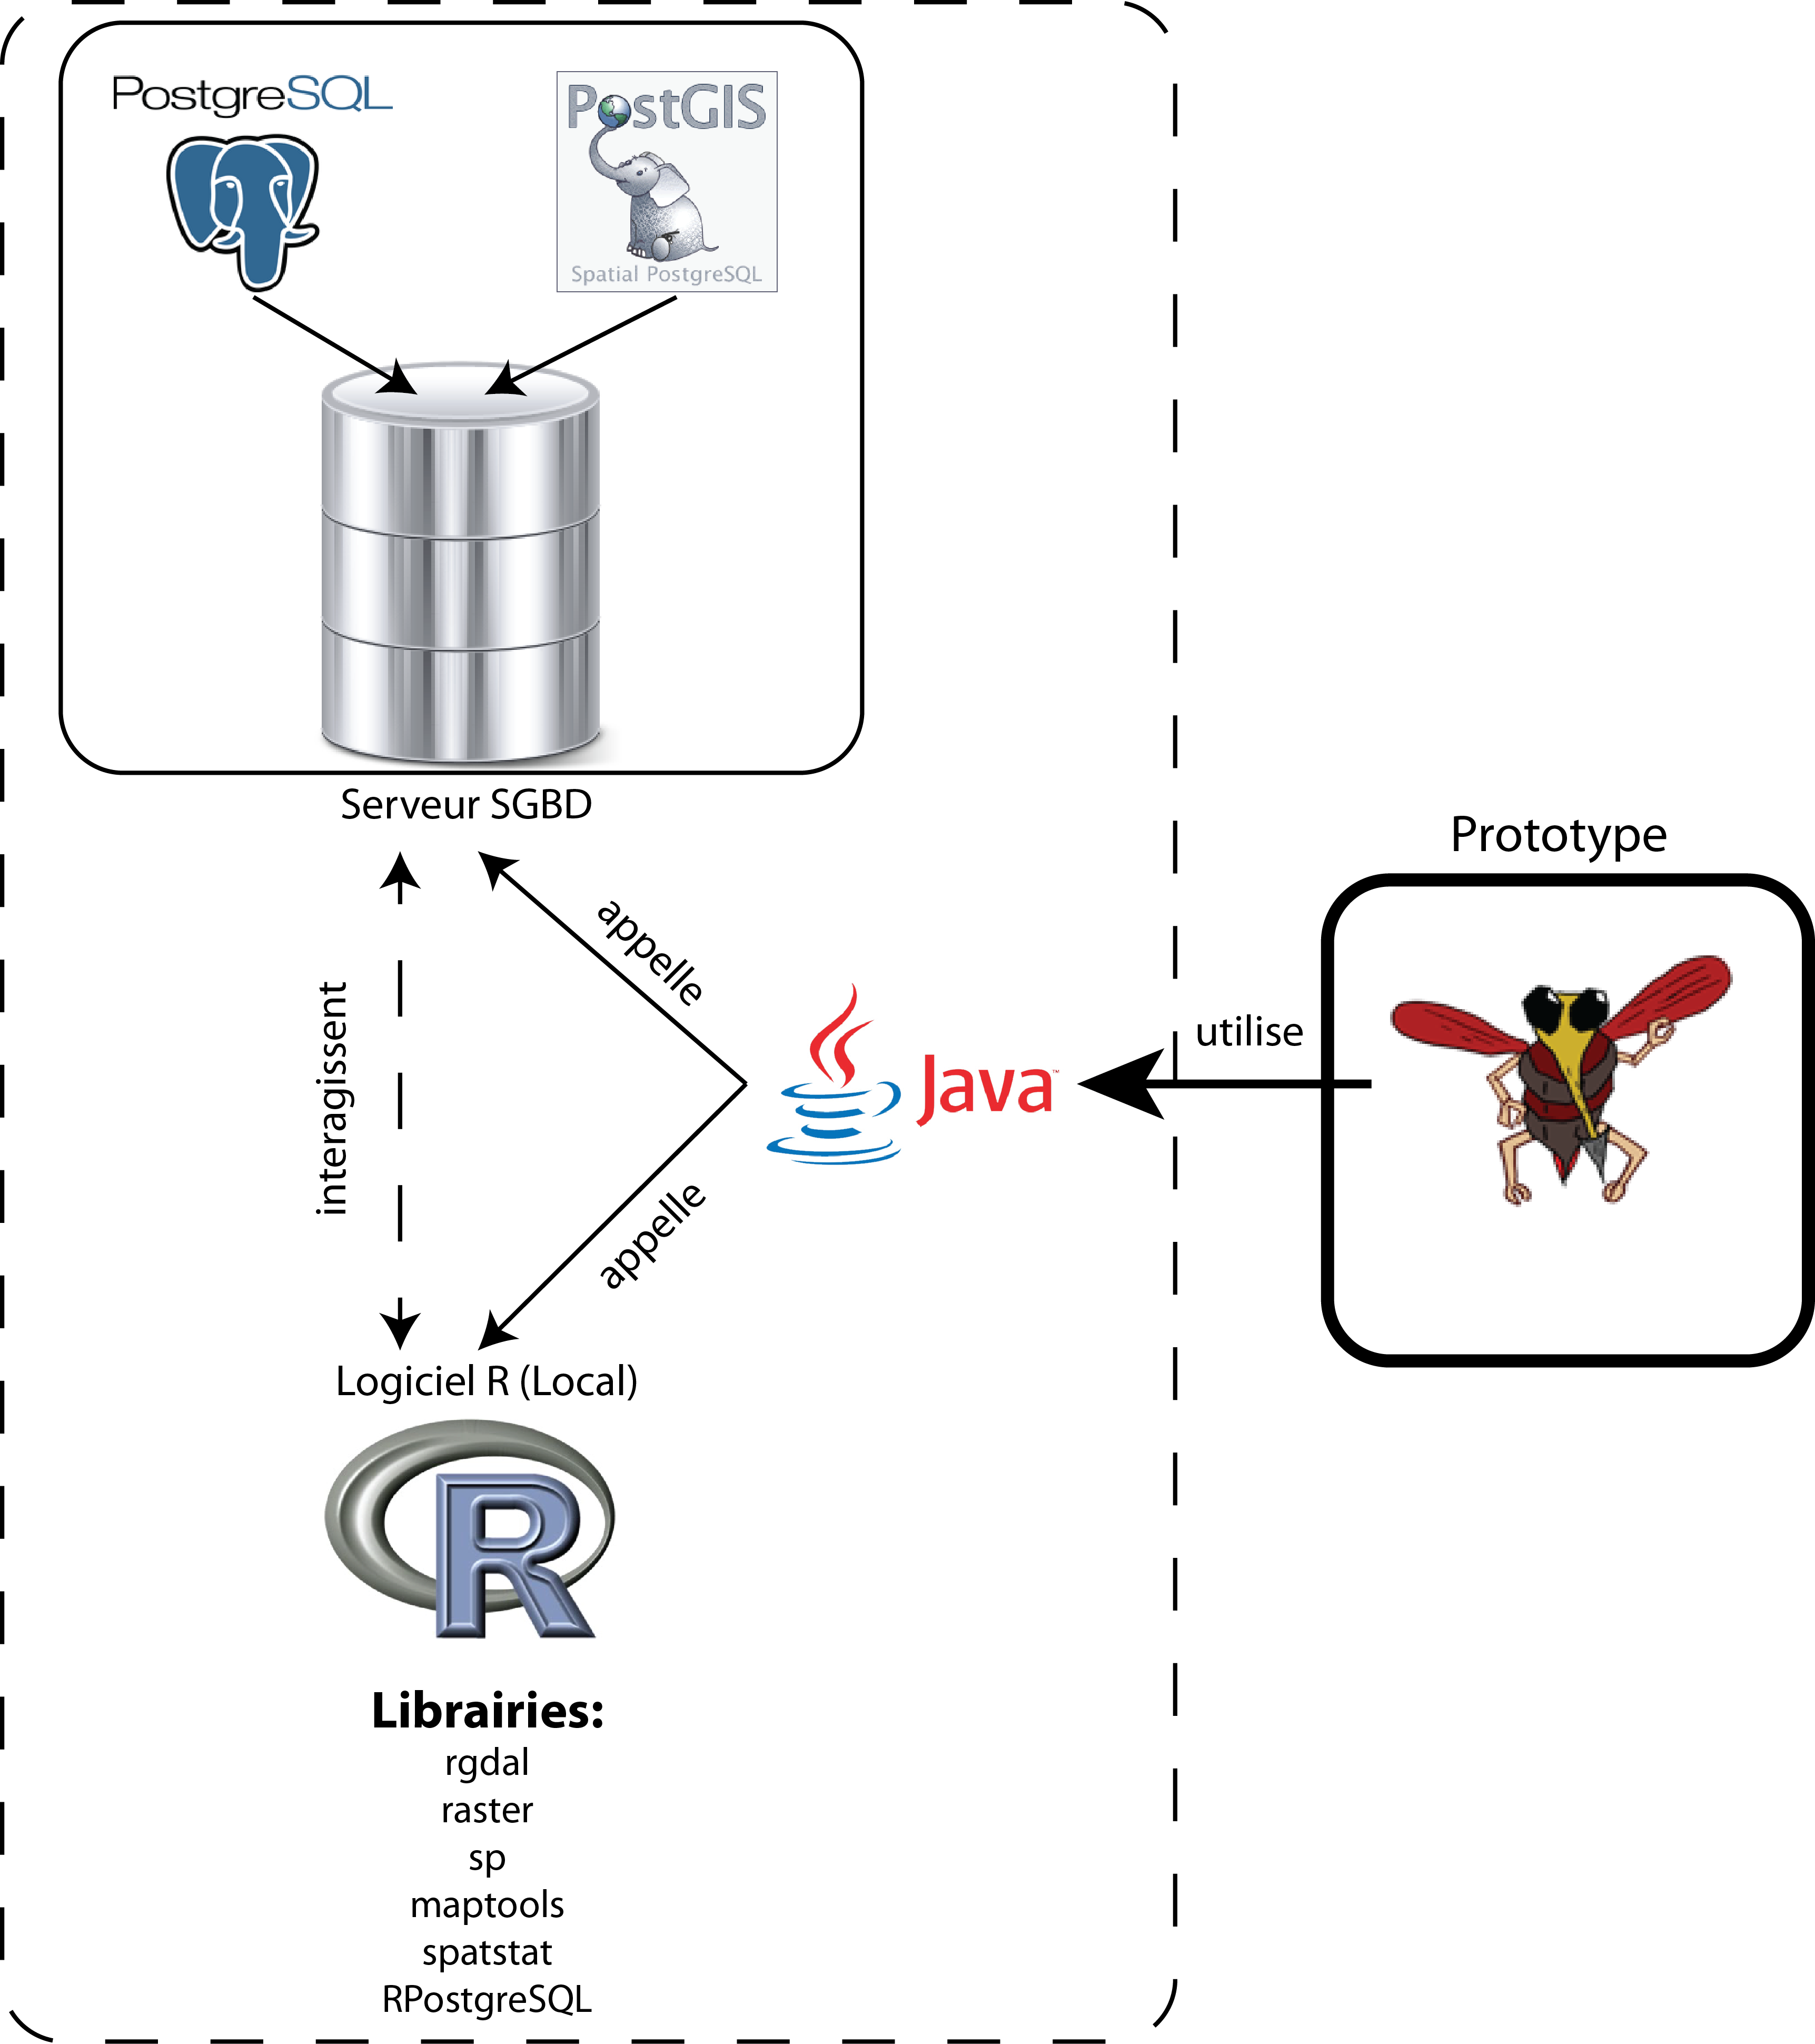
\includegraphics[width=12cm]{Architecture}\\
\caption{\label{Architecture} Architecture informatique du prototype}
\end{center}

\end{figure}


\subsubsection{Présentation de l'outil vision "fermée" (boîte noire)}

Les données utilisées sont insérées dans une base de données \textbf{PostgreSQL} (incluant l'extension \textbf{PostGIS}). Une nouvelle base de données spatiale est créée automatiquement lors de chaque exécution de la chaîne de traitements. Les différentes librairies utiliseront les données dans cette base de données et interagissent entre elles. Par exemple, des données se trouvant dans la base de données \textbf{PostgreSQL} vont être chargées dans \textbf{R} afin de permettre le calcul la densité de population de la zone d'étude.\\

L'architecture informatique est basée exclusivement sur des outils et librairies Open Source et a permis de créer un prototype générique et modulaire. Les fonctions respectivement de PostgreSQL  et de Postgis permettent d'effectuer la majorité des traitements sur des données vecteurs comme des intersections, des buffers ou des unions. Depuis la version 2.0, Postgis gère également les fichiers au format raster. Ainsi, il est désormais possible d'insérer des fichiers raster dans la base de données PostgreSQL ou de transformer des fichiers au format vecteur en format raster. Cette version de Postgis est encore en cours de développement, de nouvelles fonctionnalités raster vont certainement être rajoutées dans le futur. \\

L'outil R permet de manipuler des données aux formats différentes grâce aux nombreuses librairies disponibles pour cet outil. La librairie "spatstat" nous permet par exemple de calculer une densité de population ou d'effectuer une reclassification d'une image raster. La libraire "rgdal" nous permet de disposer des fonctionnalités de la librairie \textbf{GDAL} et de charger dans R les données raster ou vecteurs stockées dans une base de données.\\

Certaines fonctionnalités sont disponibles dans les deux outils et nous avons faits plusieurs tests pour trouver l'outil le plus pertinent par rapport à une problématique. Par exemple la transformation d'un vecteur en raster nécessite beaucoup plus de temps sous R qu'en utilisant la fonction "ST\_Raster" de PostGIS.\\

La multiplicité des fonctions disponibles avec ces deux outils, sachant qu'il existe des librairies R par rapport à de nombreuses problématiques, garantit que cette architecture pourra servir comme base pour un futur développement information du SIEL et être réutilisable par des experts de différents domaines.\\

\subsubsection{Présentation du logiciel vision "ouverte" (boîte blanche)}

Le logiciel ouvert fonctionne sur le même principe que la chaîne de traitements. Le logiciel a été développé en Java et se connecte à un \textbf{SGBD} via un \textbf{JDBC} et au logiciel R via \textbf{RCaller}. En fonction des traitements que l'utilisateur veut effectuer, le logiciel appelle les fonctionnalités PostgreSQL/PostGIS ou R.\\

Néanmoins, un certain nombre de fonctionnalités supplémentaires a été rajouté. Le logiciel est à ce jour un logiciel de création ou de gestion de données, permettant d'insérer, de créer, de modifier ou de supprimer des données dans une base de données spatiale. Ainsi, le logiciel peut intéresser un grande nombre de personnes, spécialistes et non-spécialistes dans le domaine des \textbf{SIG} ou des base de données.\\



\section{Opérationnalisation}

\subsection{Fonctionnement chaine de traitements "fermée"}


\paragraph{Choix des fichiers d'entrée\\\\}

L'utilisateur choisit les données d'entrée. Seules des données au format shape (vecteur) peuvent être sélectionnées. L'utilisateur doit choisir au moins deux fichiers de données : les données correspondant aux bâtiments et les données correspondant aux surfaces aquatiques de la zone d'étude (conformément aux facteurs de risque retenus); et au maximum cinq données (correspondant aux données dont nous disposons).\\

\begin{figure}[H]
\begin{center}
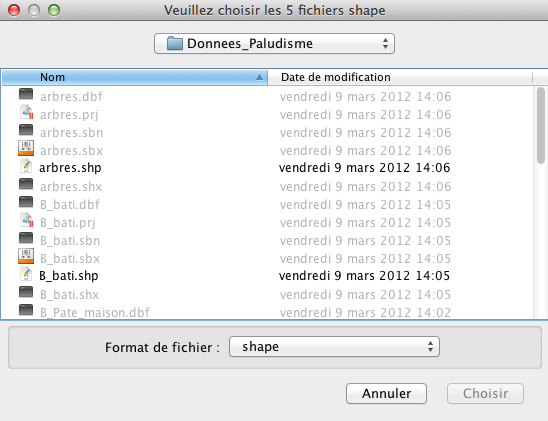
\includegraphics[width=10cm]{Chaine1}\\
\caption{\label{Chaine1} Choix fichiers d'entrée}
\end{center}
\end{figure}


\paragraph{Correspondance des couches\\\\}

Par rapport aux données sélectionnées par l'utilisateur, il est nécessaire de connaître quelle information correspond à quelle donnée. L'utilisateur choisit donc par exemple que la couche "b\_bati" correspond à l'information sur les bâtiments de la zone d'étude et la chaîne gardera en mémoire cette information pour la suite des traitements.\\

\begin{figure}[H]
\begin{center}
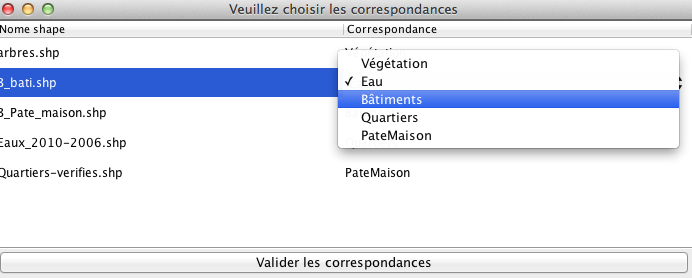
\includegraphics[width=10cm]{Chaine3}\\
\caption{\label{Chaine3} Correspondances des données}
\end{center}
\end{figure}

\paragraph{Création d'une nouvelle base de données spatiale\\\\}

La chaîne de traitements crée une nouvelle base de données. Ceci nécessite un certain nombre d'informations : l'hôte sur lequel PostgreSQL / PostGIS sont installés (localhost si installation en local sur l'ordinateur), le port sur lequel PostgreSQL / PostGIS sont installés, le nom d'utilisateur pour la base de données, le nom de la nouvelle base de données, le mot de passe et la \textbf{projection} souhaités pour la base de données.\\

\begin{figure}[H]
\begin{center}

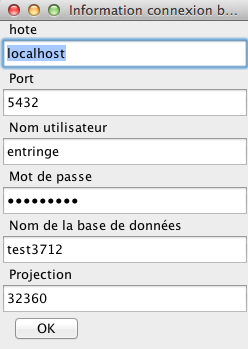
\includegraphics[width=6cm]{Chaine2}\\
\caption{\label{Chaine2} Informations création base de données}
\end{center}

\end{figure}





\paragraph{Insertion des données vectorielles dans la base de données\\\\}

A l'aide du module de transformation shp2pgsql les données vectorielles sont insérées dans la base de données. Ce module transforme les fichiers au format ".shp" en fichiers ".sql" qui sont par la suite insérés dans la base de données à l'aide de la fonctionnalité "pgsql".\\

\begin{figure}[H]
\begin{center}
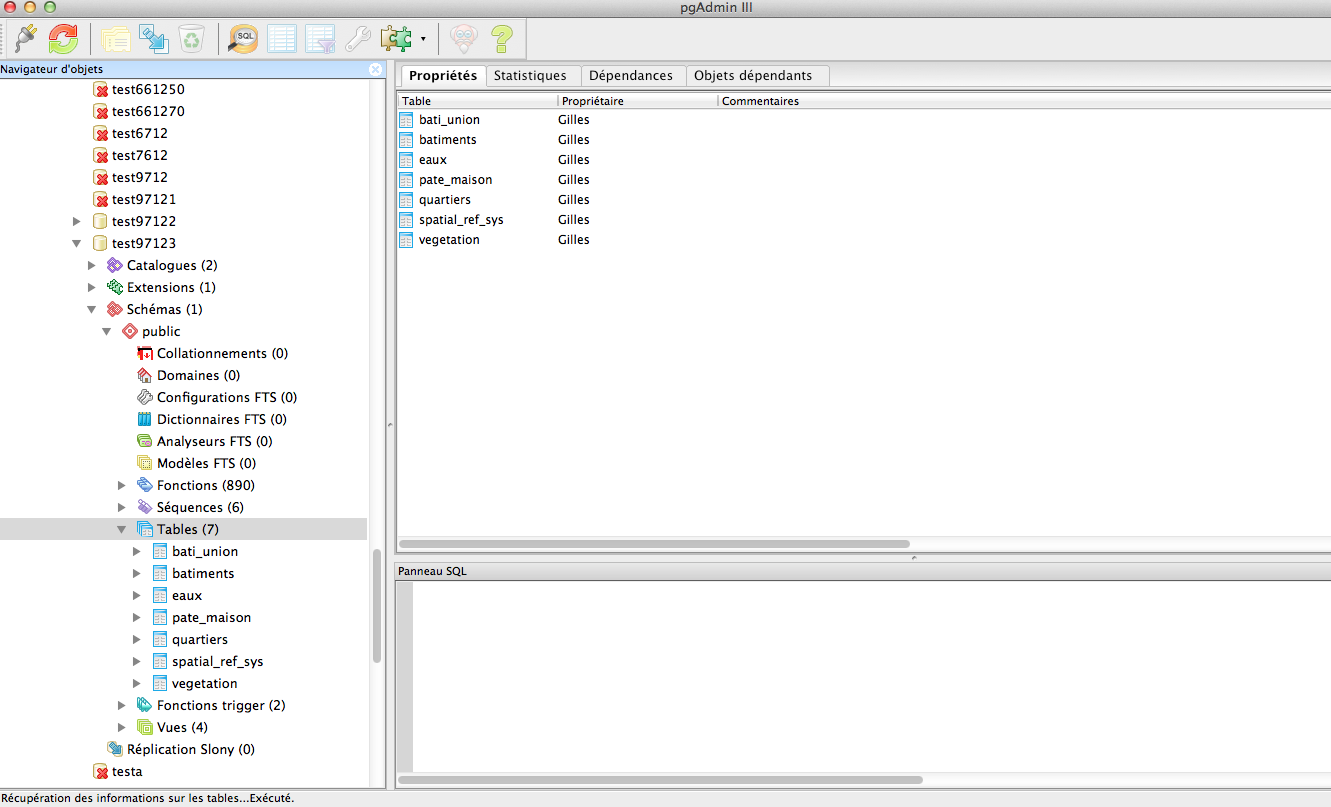
\includegraphics[width=10cm]{Chaine4}\\
\caption{\label{Chaine4} Base de données avec données insérées}
\end{center}
\end{figure}


\paragraph{Nombre d'habitants\\\\}

L'outil demande à l'utilisateur le nombre d'habitants pour la zone d'étude.\\

\begin{figure}[H]
\begin{center}
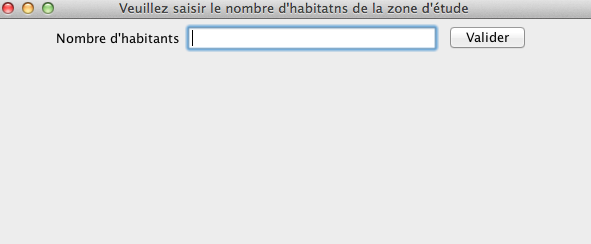
\includegraphics[width=10cm]{Chaine5}\\
\caption{\label{Chaine5} Nombre d'habitants}
\end{center}
\end{figure}


\paragraph{Calcul densité de population et taille pixel\\\\}

L'outil calcule automatiquement, à partir de la couche qui correspond aux bâtiments, la densité de population de la zone d'étude et la taille de cellule qu'un habitant occupe en théorie. Par exemple, pour une population de 15.000 habitants sur une superficie totale de 300.000 mètre carrés, nous effectuons le calcul suivant: \\

300.000/15.000 = 20 m2 par habitants\\
1 habitant = √(20)
1 habitant = 1 cellule = 4.47 * 4.47 m

Un habitant correspond donc en théorie à 20 mètres carrés et à une taille de cellule théoriques de 4.47 * 4.47 mètres.\\


\begin{figure}[H]
\begin{center}
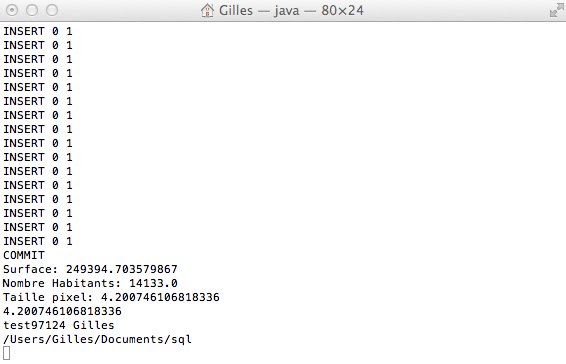
\includegraphics[width=10cm]{Chaine6}\\
\caption{\label{Chaine6} Taille de cellule / Densité de population}
\end{center}
\end{figure}

\paragraph{Calcul et affichage carte de vulnérabilité\\\\}

A partir des différentes opérations et calculs, l'outil calcule une densité des points, affiche et stocke une carte de vulnérabilité.\\

\begin{figure}[H]
\begin{center}
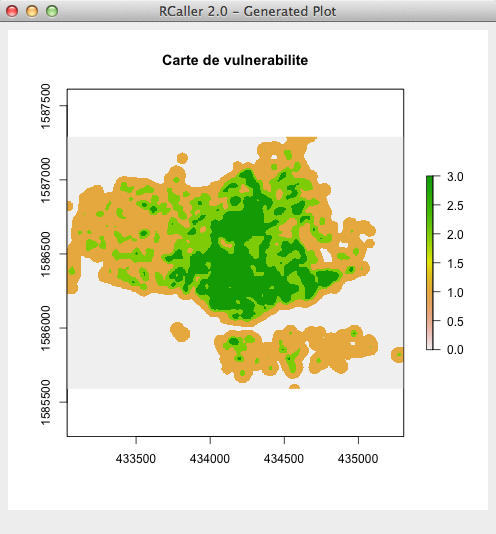
\includegraphics[width=7cm]{Chaine7}\\
\caption{\label{Chaine7}Carte de vulnérabilité}
\end{center}
\end{figure}


\paragraph{Suppression des surfaces aquatiques polluées\\\\}

Par rapport aux données que nous possédons, il est nécessaire de supprimer des surfaces aquatiques polluées car les moustiques ne peuvent pas survivre dans les eaux polluées. L'outil permet de sélectionner quelles surfaces sont polluées à partir d'une colonne de la \textbf{table} de la base de données qui permet à l'utilisateur d'identifier ces surfaces. \\


\begin{figure}[H]
\begin{center}
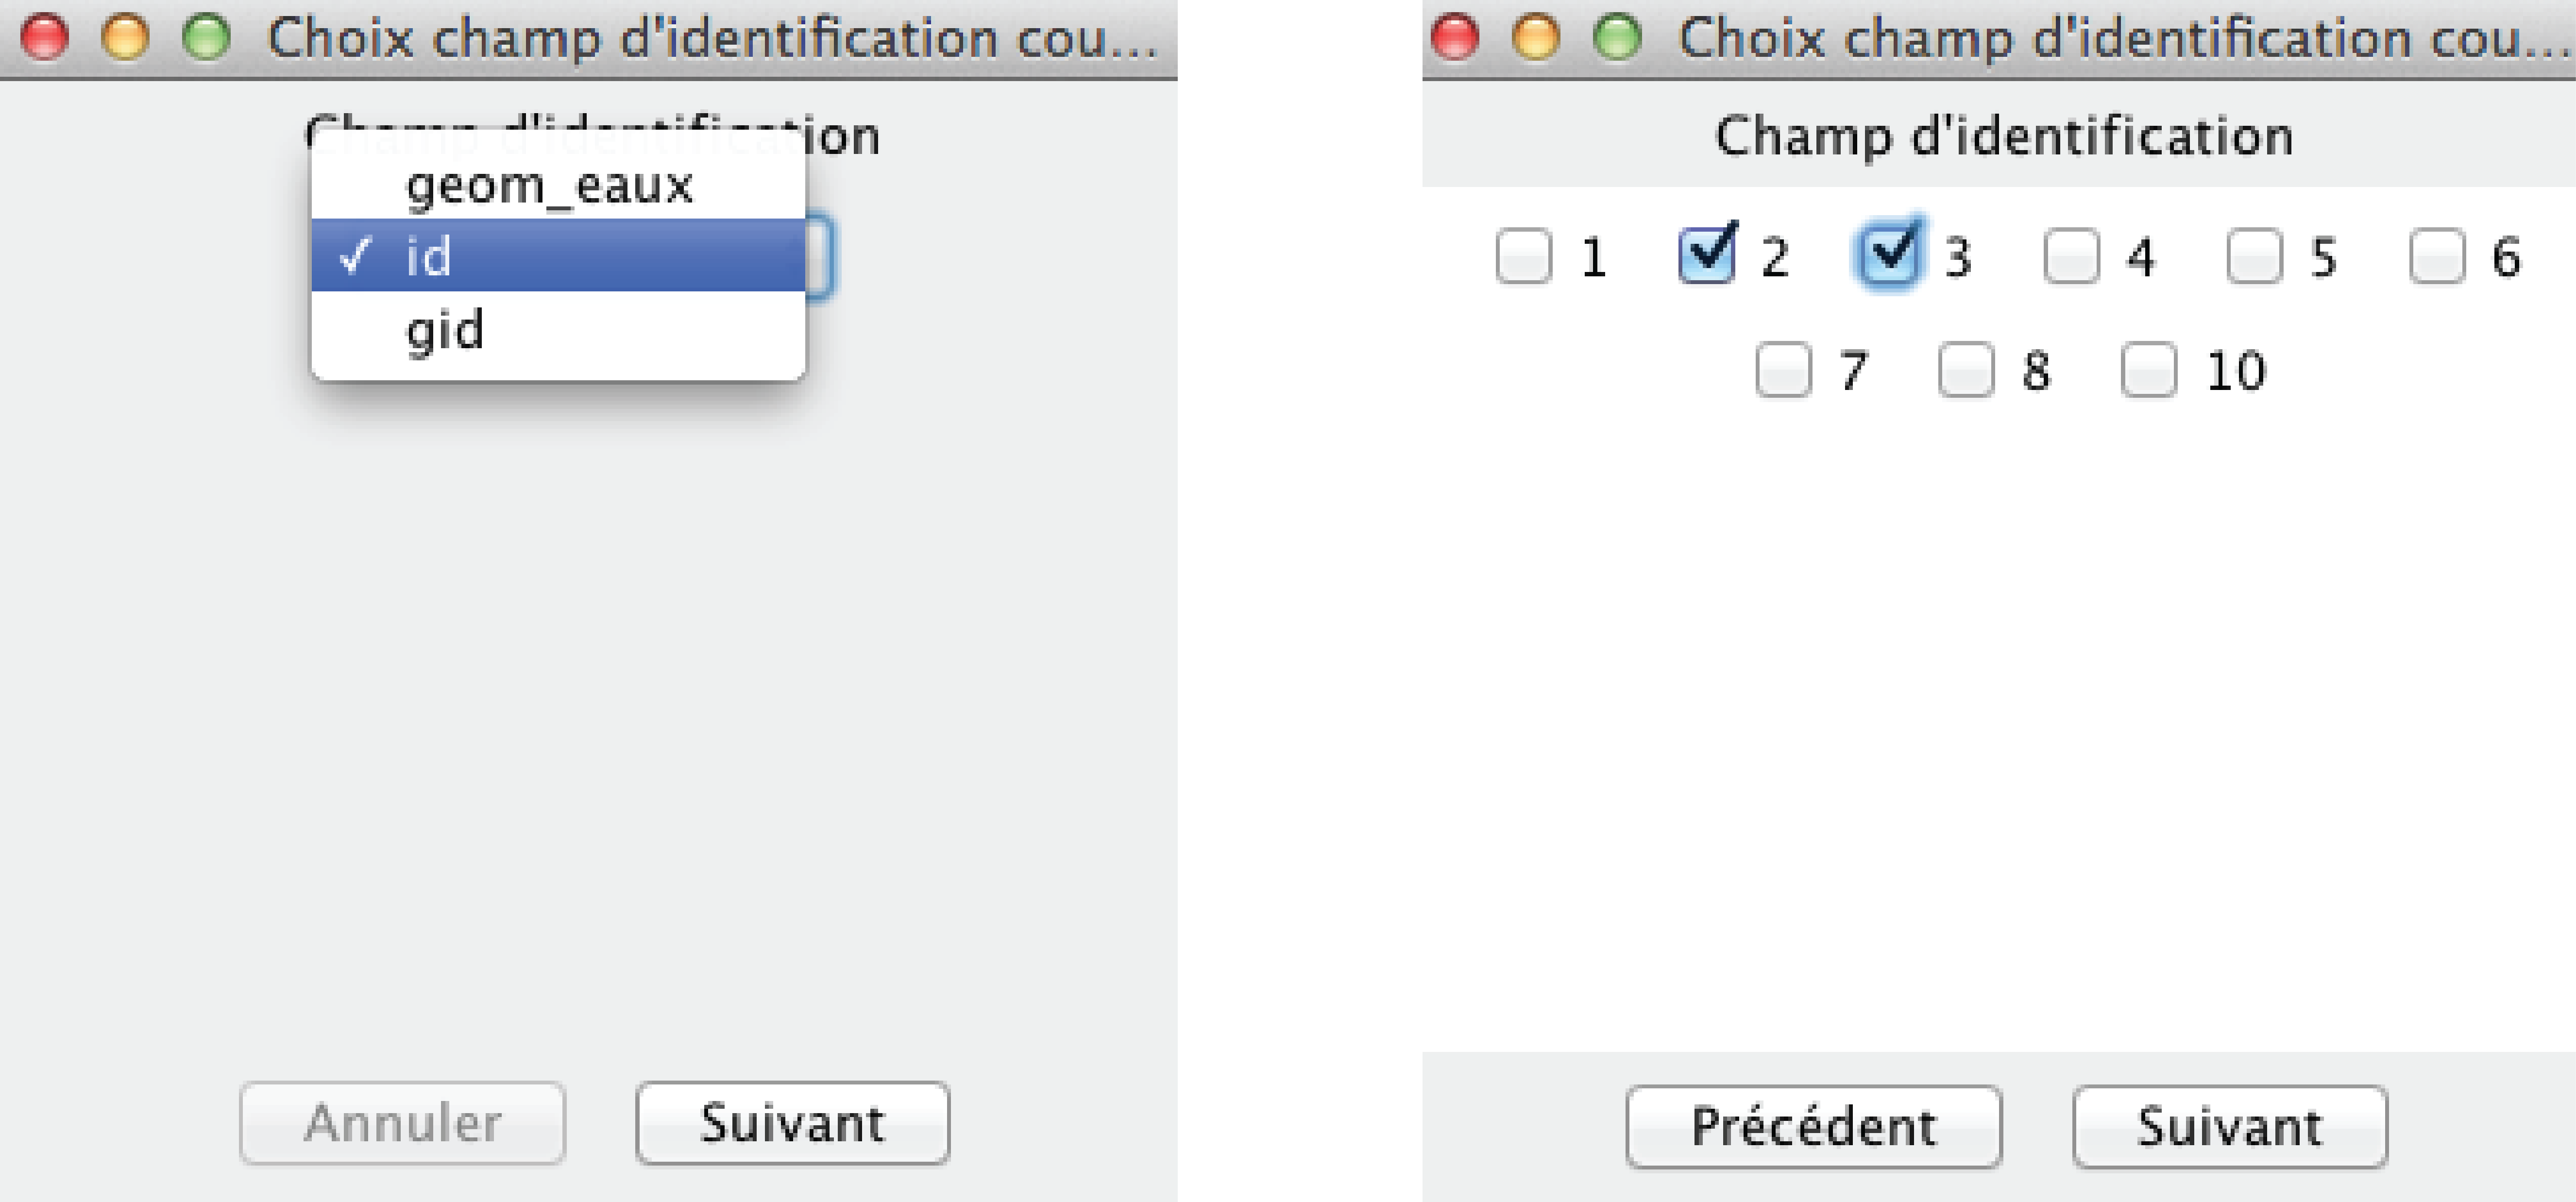
\includegraphics[width=13cm]{Chaine13}\\
\caption{\label{Chaine13}Supprimer surfaces aquatiques polluées}
\end{center}
\end{figure}



\paragraph{Carte d'aléa\\\\}

La carte d'aléa est calculée en combinant plusieurs opérations et traitements d'analyse spatiale : Intersection, création de \textbf{zones tampon}, Union, extent (emprise géographique). Comme il n'y aura pas de risque dans les zones où il n'y pas de vulnérabilité, il est intéressant de supprimer les parties concernant l'aléa qui n'intersectent pas avec la carte de vulnérabilité. Finalement nous obtenons donc une carte d'aléa. Cette carte, en combinaison avec la carte de vulnérabilité crée une carte de risque de transmission, affichée à la fin du traitement.

\begin{figure}[H]
\begin{center}
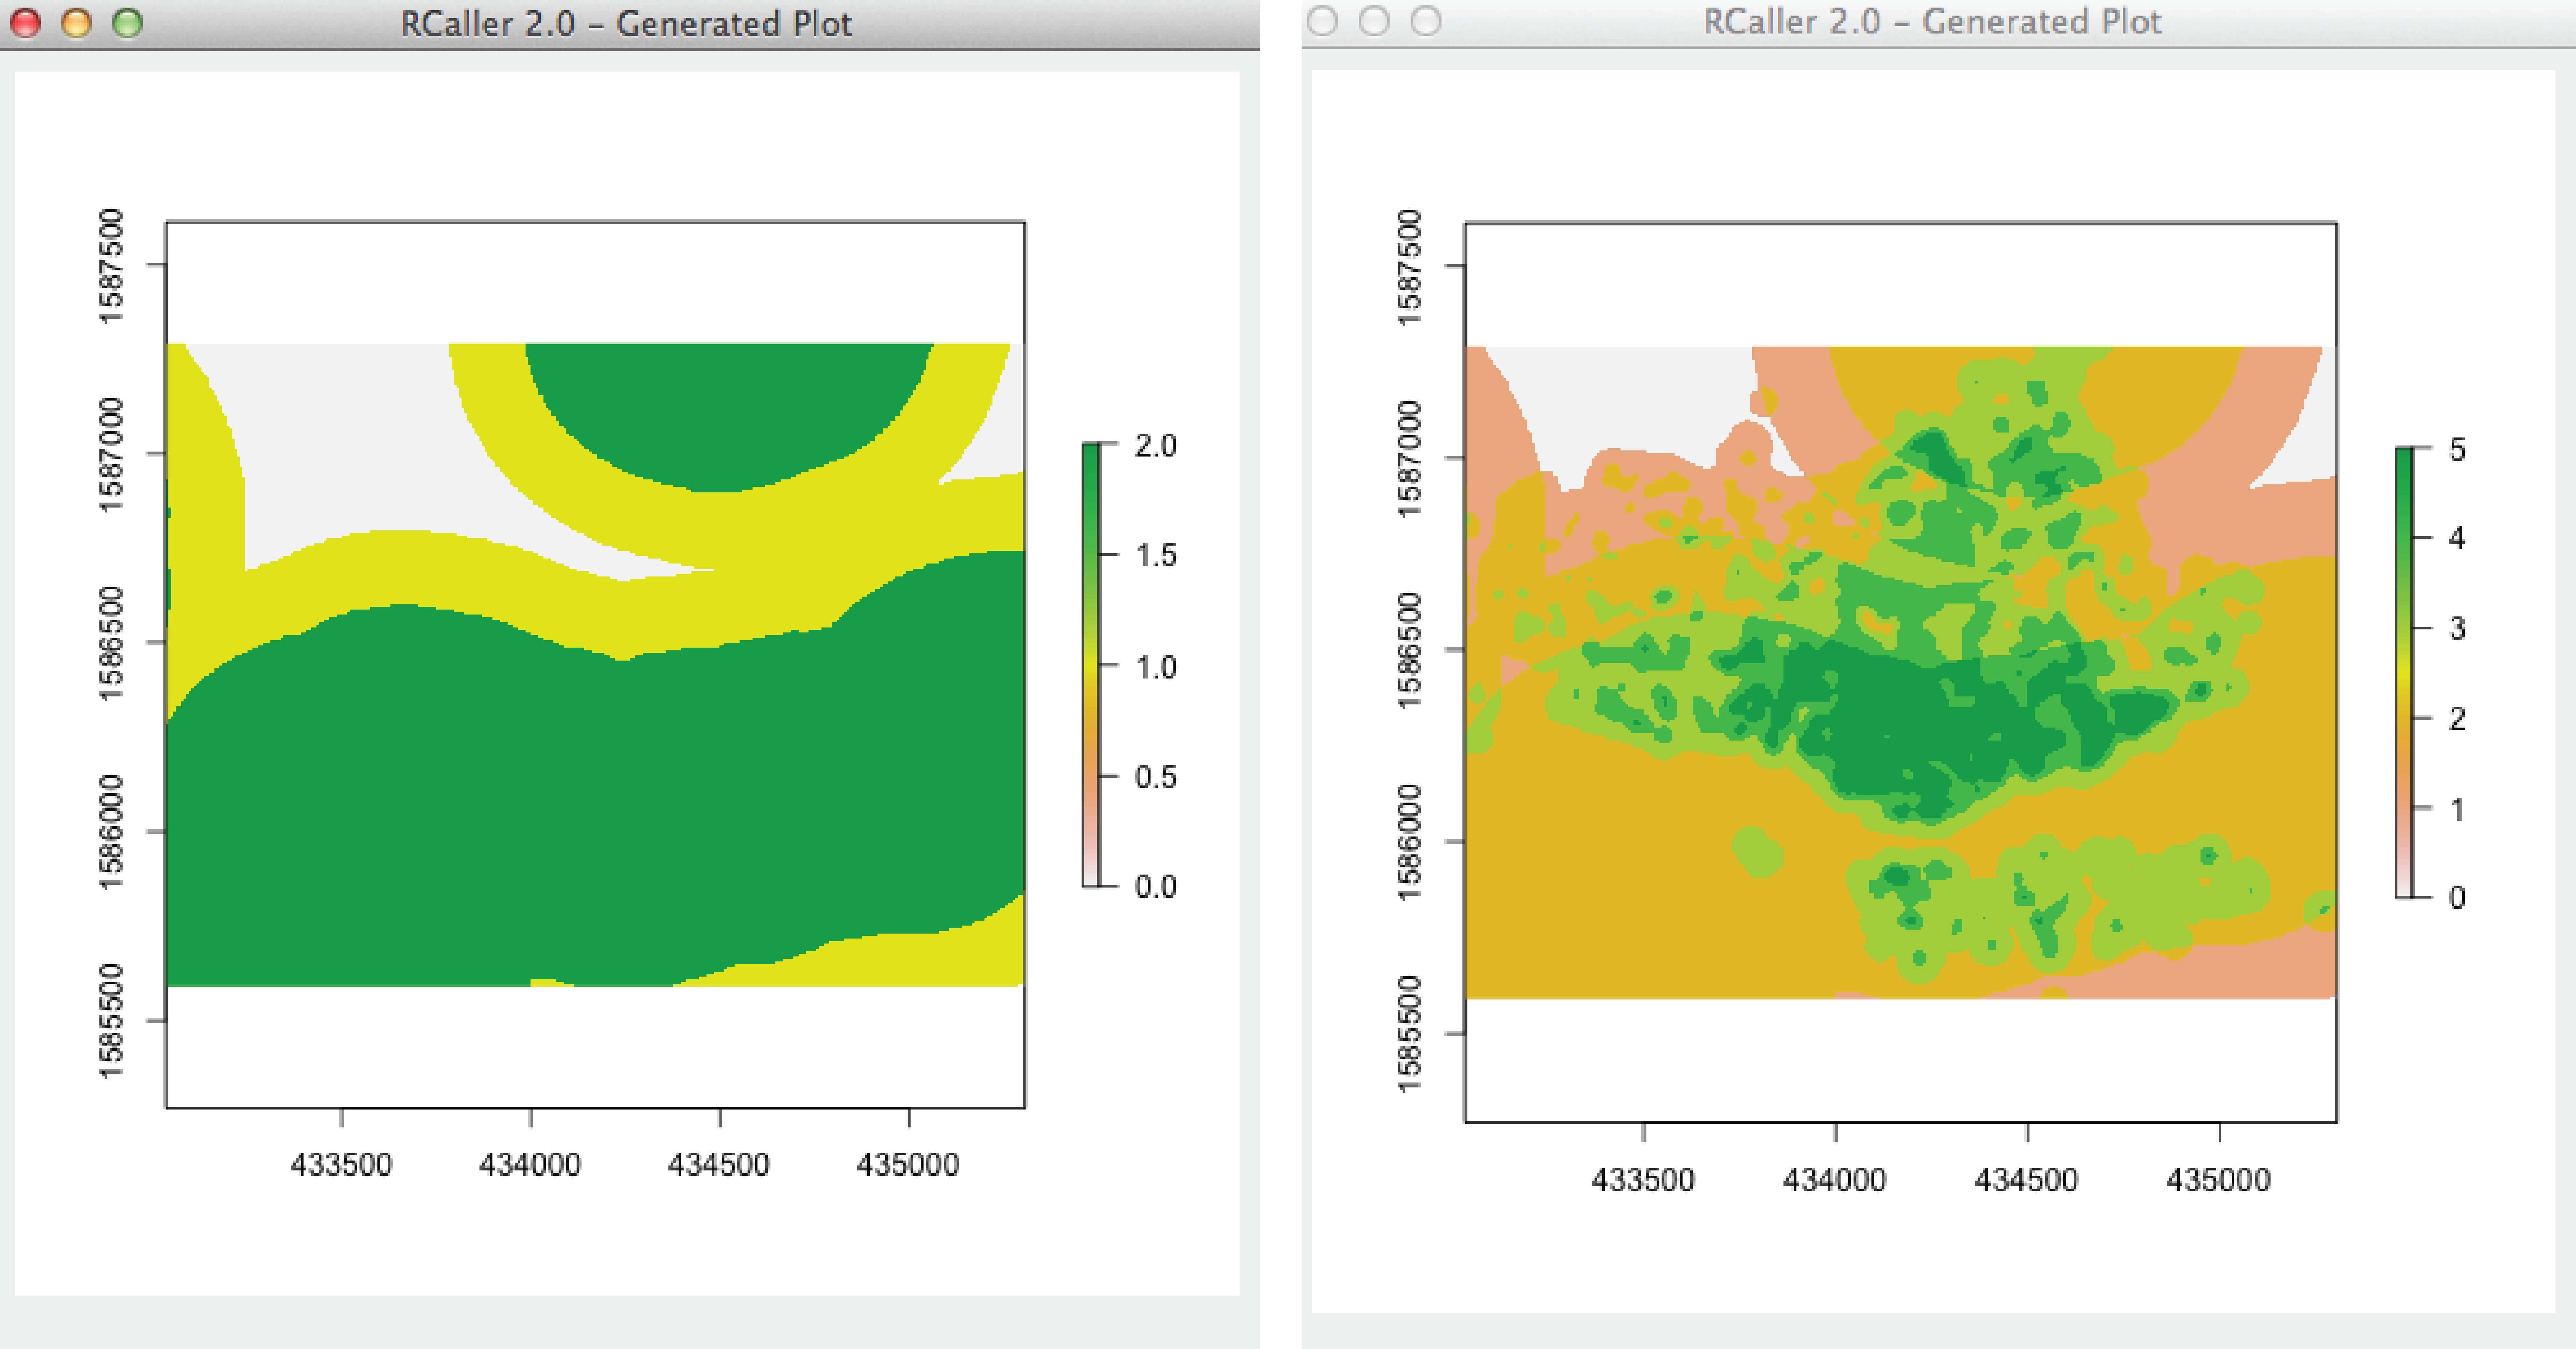
\includegraphics[width=13cm]{Chaine12}\\
\caption{\label{Chaine12}Exemple de carte d'aléa et carte de risque}

\end{center}
\end{figure}

\newpage

%%\subsection{Architecture informatique du logiciel ouvert}

\subsection{Fonctionnement du logiciel "ouvert"}

Le l\textbf{ogiciel ouvert} utilise les mêmes librairies et bibliothèques (R, PostGis, PostgreSQL) que la chaîne de traitements fermée. Au fur et à mesure de l'avancement du développement du logiciel, nous avons rajouté certaines fonctionnalités que nous avons jugées importantes pour l'utilisation du logiciel, comme par exemple l'export des données ou la possibilité de renommer les tables de la base de données. Dans cette partie sera illustrée l'implémentation de l'outil à partir des fonctionnalités les plus intéressantes et innovantes.

\paragraph{Choix emplacement des données\\\\}

L'utilisateur dispose de trois choix possibles par rapport à l'emplacement des données qu'il souhaite traiter :

\begin{itemize}

\item Données dans une base de données PostGIS existante : les données stockées dans la base sont utilisées 
\item Données sur disque dur : une nouvelle base de données est créée
\item Données sur disque dur et dans base de données : des données sont insérées dans une base de données existantes
\end{itemize}


\begin{figure}[H]
\begin{center}
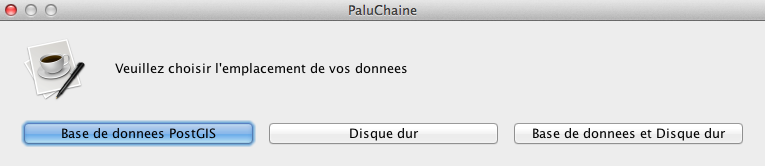
\includegraphics[width=10cm]{Logiciel1}\\
\caption{\label{Traitement1}Choix de l'emplacement des données}

\end{center}
\end{figure}

\paragraph{Information connexion base de données\\\\}

L'utilisateur indique les informations relatives à la base de données. En fonction du choix précédent (emplacement des données), les données stockées dans une base de données existante sont chargées ou une nouvelle base de données est créée et les données des fichiers sélectionnées par l'utilisateur y sont stockées. De plus, l'utilisateur indique la projection de la base de données. Lors de la création d'une nouvelle base de données, toutes les données sont projetées par rapport à cette information, dans le cas d'une base de données existante, toutes les données stockées dans la base sont analysées et, si nécessaire, reprojetées.

\begin{figure}[H]
\begin{center}
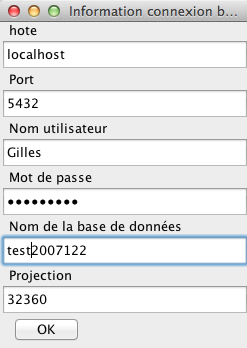
\includegraphics[width=4cm]{Logiciel2}\\
\caption{\label{Traitement2}Informations base de données}
\end{center}
\end{figure}

\paragraph{Menu du logiciel\\\\}

Un menu présente les différents traitements en fonction des catégories de traitements définies  auparavant (cf. \ref{catdonnees}). L'utilisateur peut choisir indépendamment les traitements qu'il souhaite effectuer. 

\begin{figure}[H]
\begin{center}
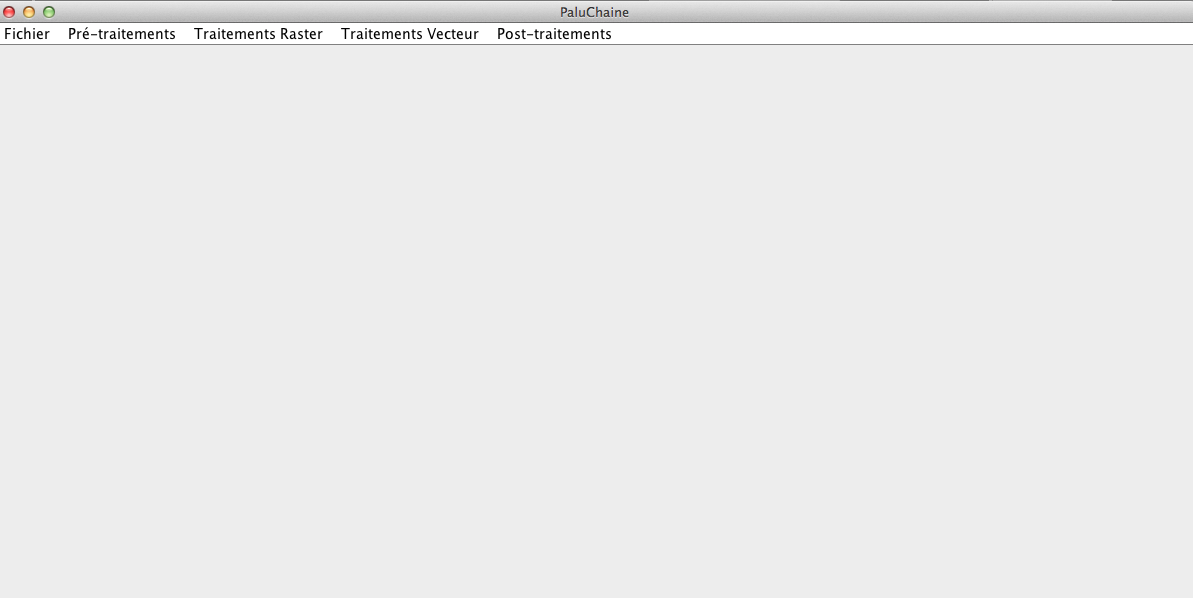
\includegraphics[width=12cm]{Logiciel3}\\
\caption{\label{Traitement2}Le menu de l'outil}
\end{center}
\end{figure}


\paragraph{Les traitements possibles\\\\}

En fonction des catégories de traitements définies auparavant, les traitements suivants peuvent être effectués :

\textbf{Pré-traitements:}\\

\begin{itemize}
\item Insertion de données raster et  vecteur dans la base de données
\item Suppression de données  raster et  vecteur stockées dans la base de données\\

\textbf{Traitements:}\\\\
\textit{Analyse Spatiale}
\item Intersection entre des couches vecteurs
\item Union entre des couches vecteurs
\item Création des zones tampons
\item Calcul de la différence entre deux couches vecteur
\item Création d'une couche représentant l'emprise d'une couche\\\\ \textit{Statistique}
\item Calcul de la surface totale d'une couche
\item Calcul de la taille théorique d'une cellule (cf. Chaîne de traitements)
\item Calcul d'une densité des points à partir d'une couche vecteur\\\\
\textit{Transformation}

\item Rastérisation de couches vecteurs
\item Changement de la projection de la base de données\\

\textbf{Post-traitements}\\
\item Suppression de certaine information d'une couche
\item Reclassification un raster
\item Combinaison de plusieurs rasters
\item Renommage des données dans la base (raster et vecteur)
\item Visualisation de données vecteur et  raster
\end{itemize}


\paragraph{Spécificités techniques du logiciel}

\subparagraph{Mémoire\\\\}

Le logiciel mémorise les traitements déjà effectués (et ce à des fins de contrôle). Par exemple, il n'est pas possible de calculer une taille théorique d'une cellule sans calculer la surface totale de la donnée auparavant. Lorsque l'utilisateur a calculé la taille de cellule et  veut rastériser une donnée au format vecteur, le logiciel se rappelle du calcul de la cellule effectué auparavant. L'utilisateur peut bien évidemment également saisir manuellement la taille de pixel qu'il souhaite appliquer pour le traitement. \\

Après avoir calculé la superficie pour une donnée, elle n'apparaît plus dans la liste des données disponibles pour effectuer ce traitement. Il en est de même pour le calcul de la taille de pixel.

\subparagraph{Affichage\\\\}

L'utilisateur peut afficher à tout moment les données stockées dans la base de données. Cet affichage se fait sous la forme de la fonctionnalité "plot" du logiciel R. 

\subparagraph{Exporter des données\\\\}

Les données stockées dans la base de données peuvent être exportées. Exemple : L'utilisateur, après avoir créé des zones tampons, peut exporter cette nouvelle donnée (au format shape) et l'utiliser dans le SIG de son choix.

\subparagraph{Gestion des données\\\\}

A tout moment, des nouvelles données (vecteur ou raster) peuvent être insérées dans la base de données. Il est également possible de supprimer des données et de renommer les données (tables).

\paragraph{Aperçus du logiciel ouvert\\\\}

La figure \ref{aperculogiciel} donne un bref aperçu du logiciel et de ses fonctionnalités. 
 
\newpage



\begin{figure}[H]
\begin{center}
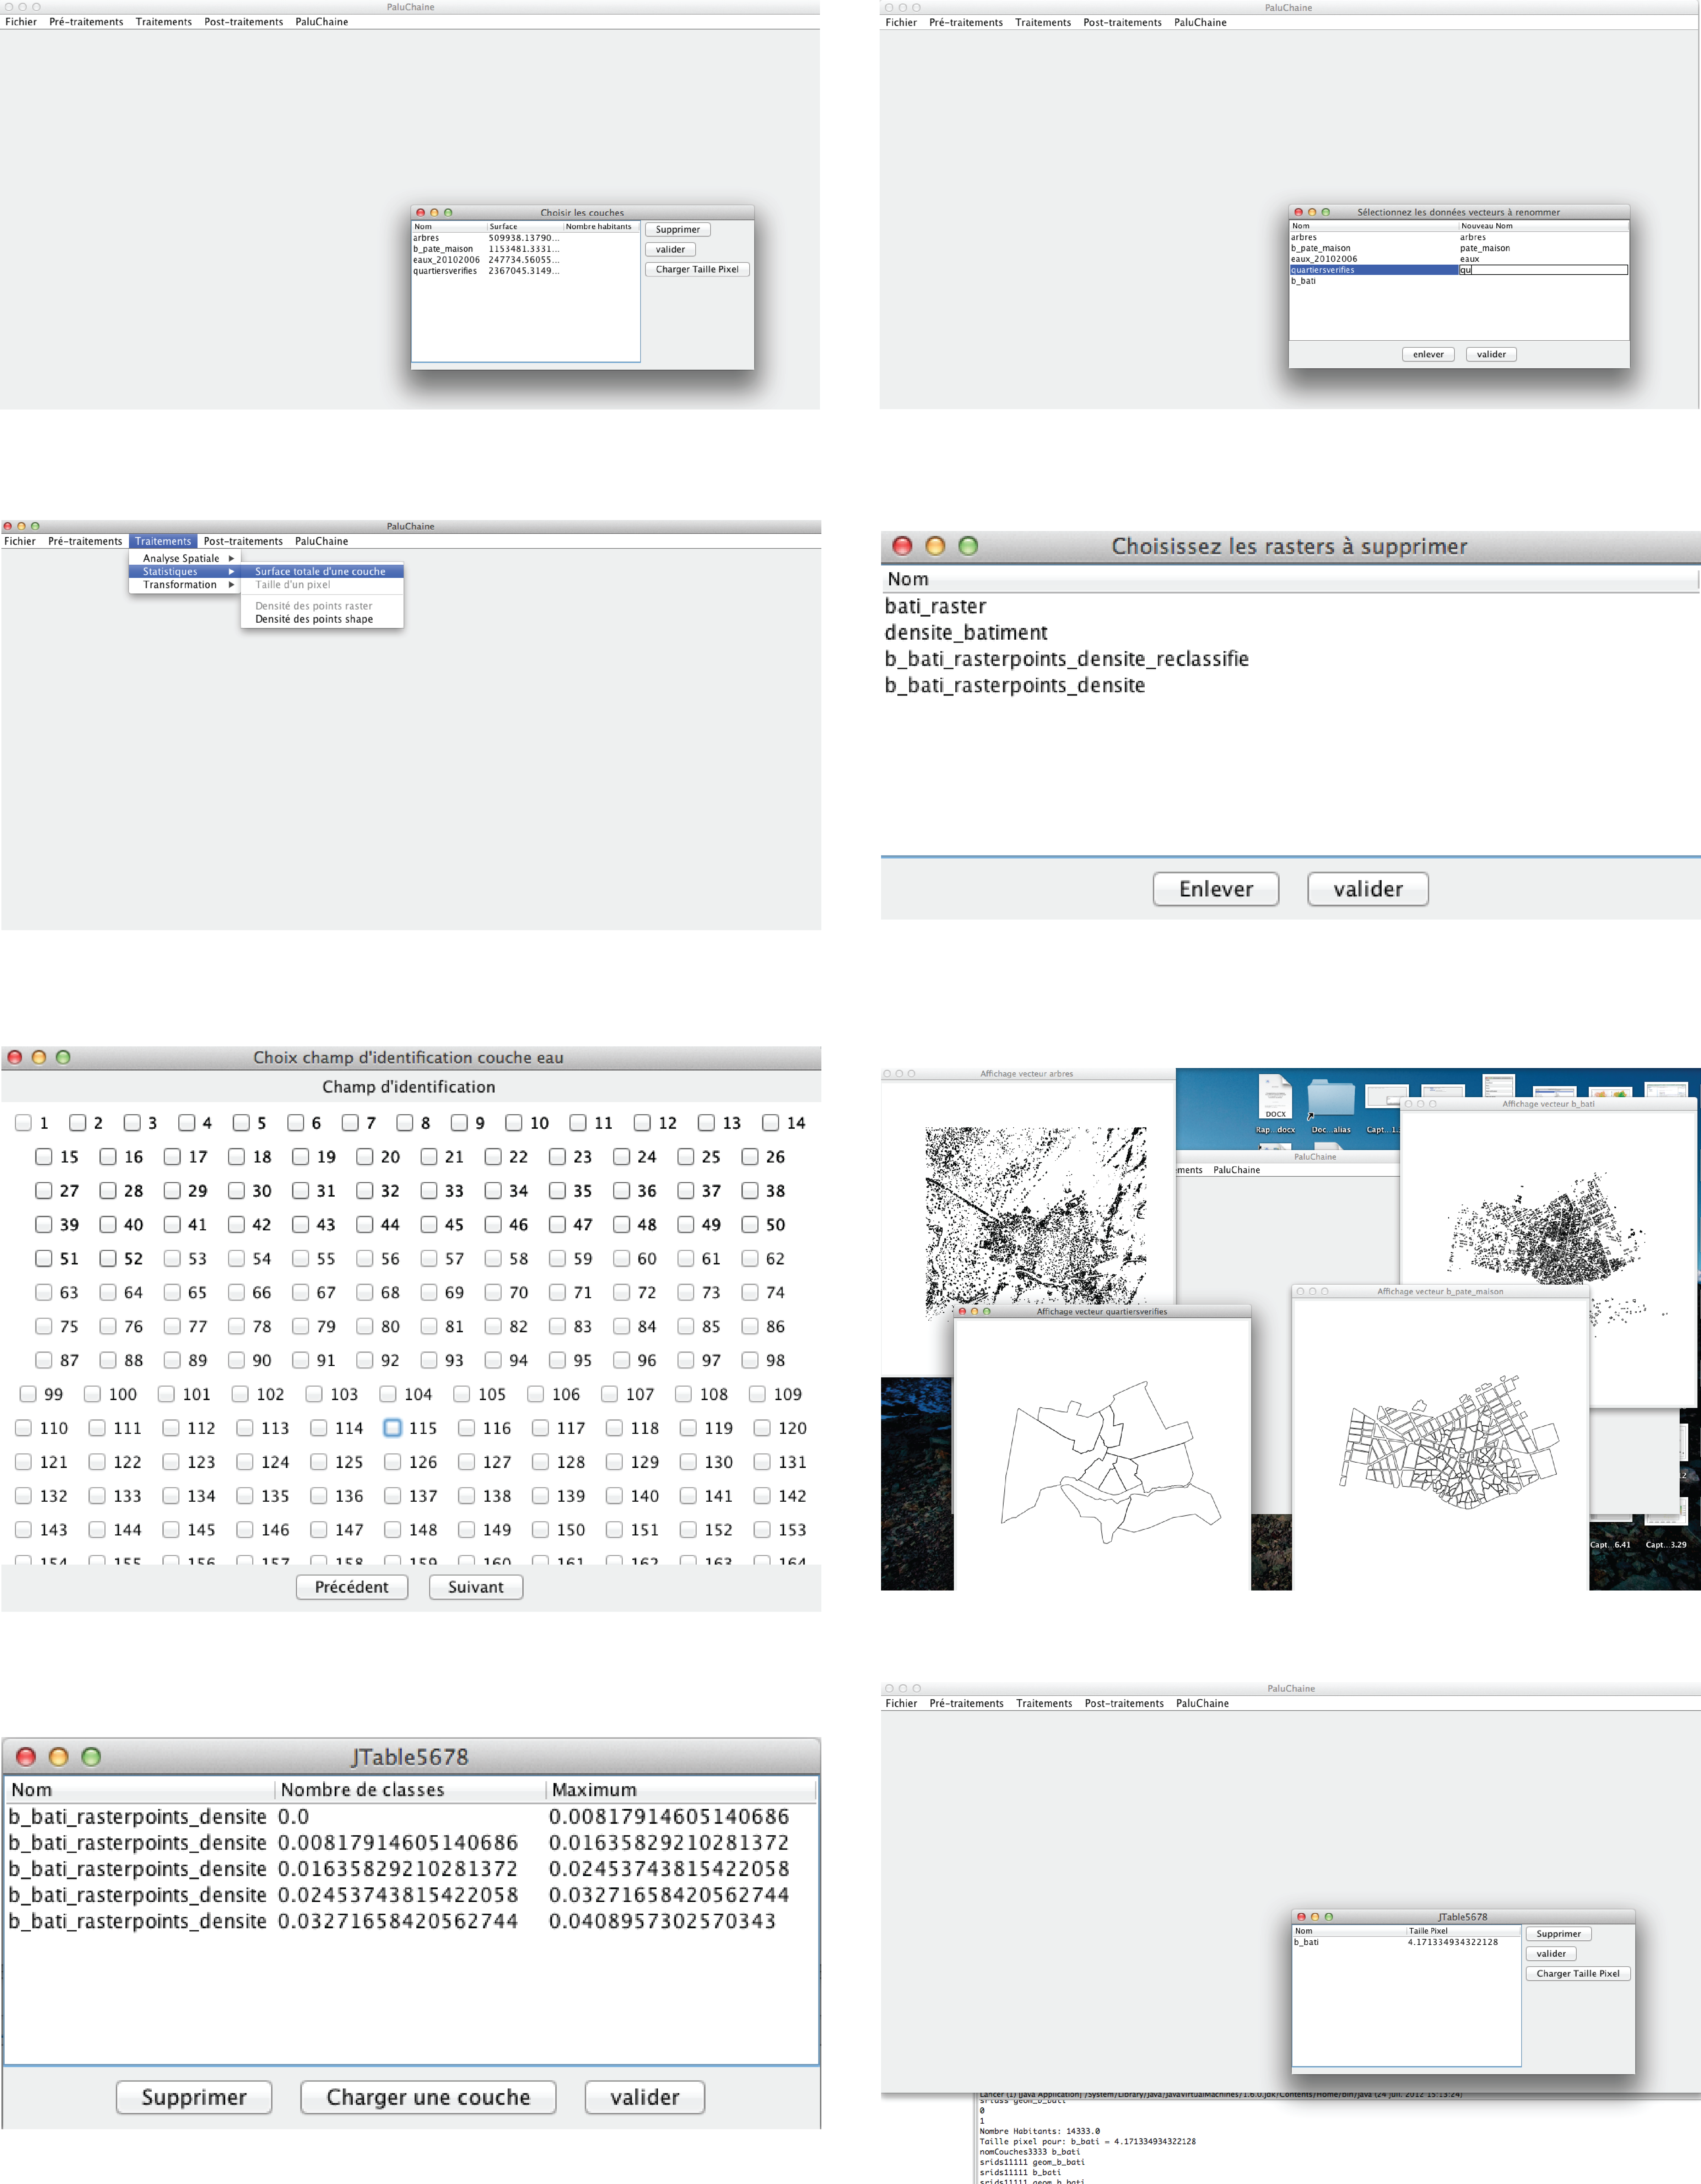
\includegraphics[width=17cm]{Logiciel}\\
\caption{\label{aperculogiciel}Aperçus du logiciel libre}
\end{center}
\end{figure}








\chapter{Résultats} \label{Resultats}

\section{Planning final }

Le diagramme de Gantt (cf. \ref{GanttFinal}) montre le planning final de mon stage. Contrairement au planning élaboré en début de stage, la chaîne de traitements était déjà opérationnel au bout de quatre mois de travail et nous avons pu réadapter nos objectifs et développer en plus un logiciel ouvert.

\begin{center}
\begin{figure}[h] \centering
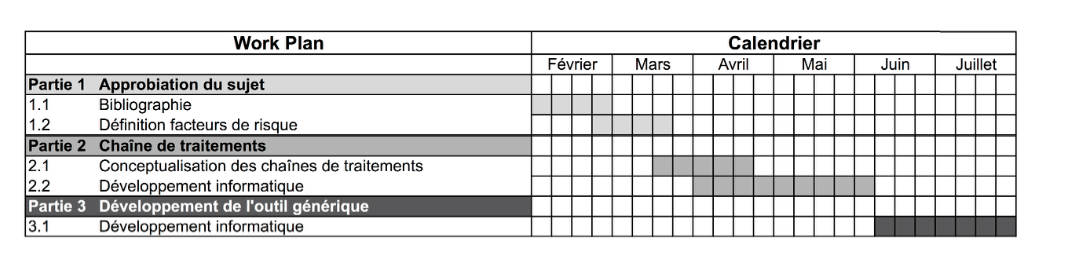
\includegraphics[width=14cm]{GanttFinal}\\
\caption{\label{GanttFinal} Planning final }
\end{figure}
\end{center}

\section{Prototype }

Nous avons développé deux outils, basés sur des plateformes Open Source. Le premier outil, une chaîne de traitements automatisée fermée qui permet d'effectuer des traitements dans un ordre bien défini pour cartographier des indicateurs de risque environnemental. Le deuxième outil, un \textbf{logiciel ouvert}, donne à l'utilisateur la possibilité d'exécuter et de combiner chacun des traitements de la chaîne selon  ses besoins. 

\begin{center}
\begin{figure}[h] \centering
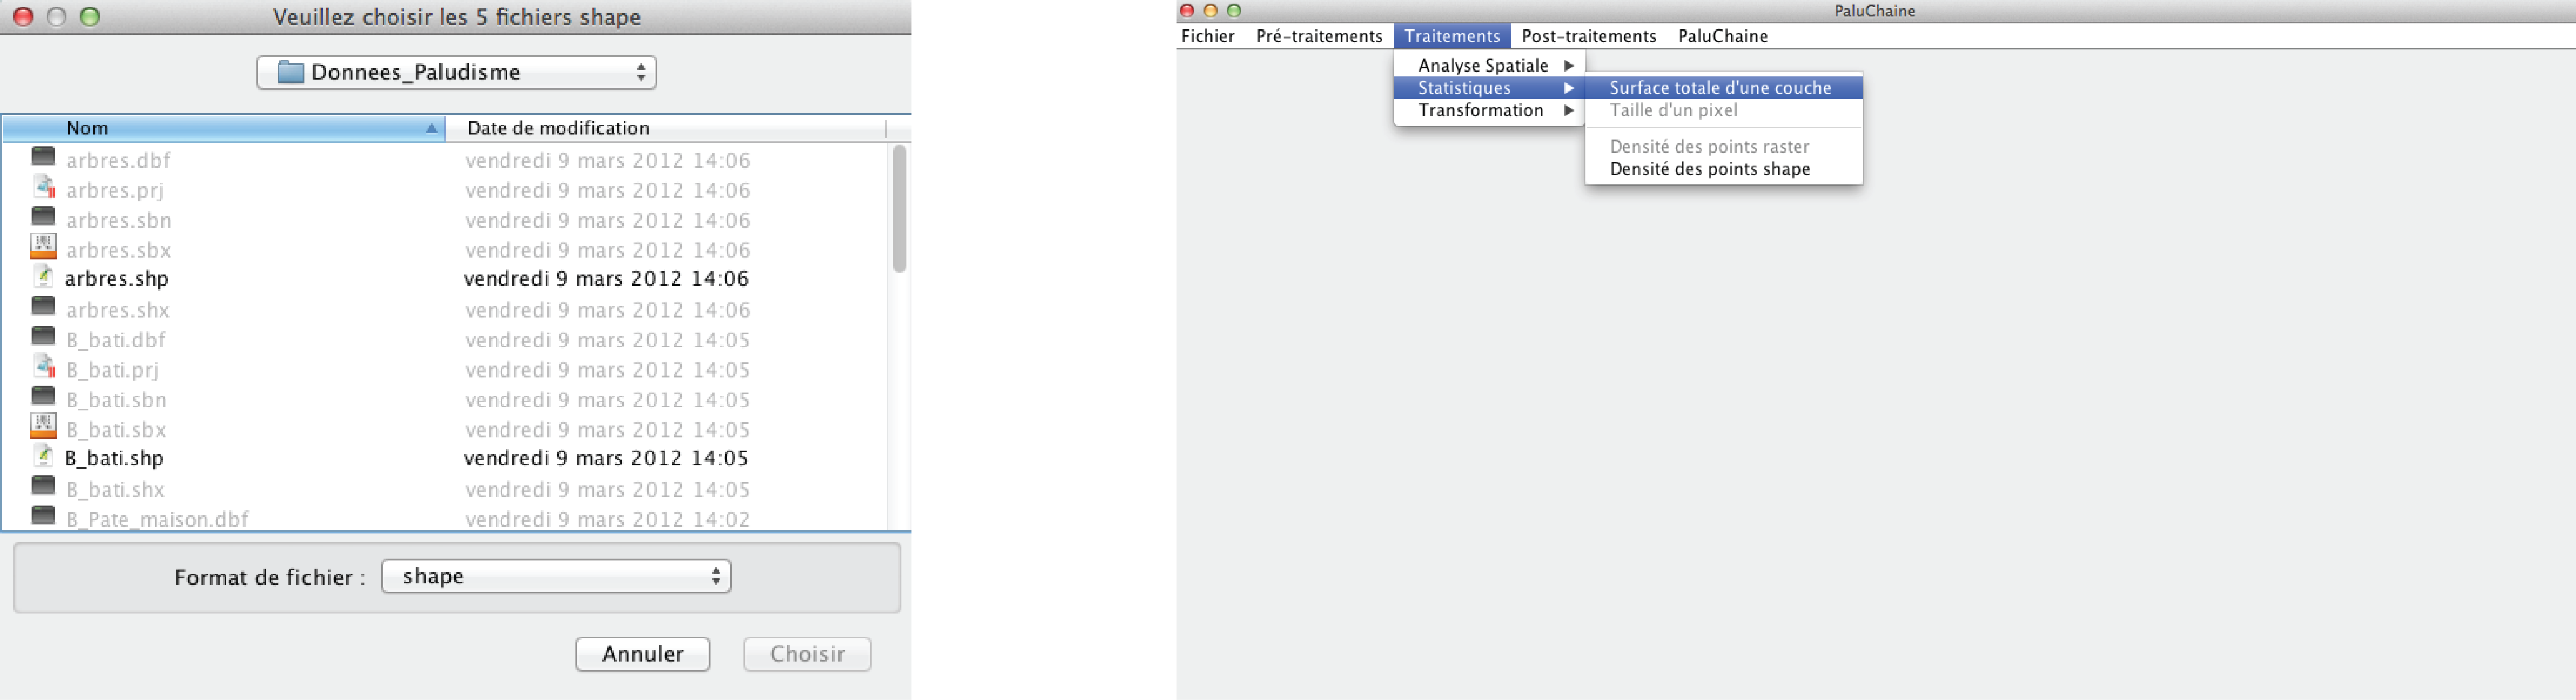
\includegraphics[width=14cm]{Results}\\
\caption{\label{Results} Aperçus des deux outils ("ouvert à droite) }
\end{figure}
\end{center}

\section{Validation des résultats}

Pour valider les résultats et surtout le fonctionnement de la chaîne de traitements, nous comparons une carte de vulnérabilité, une carte d'aléa et une carte de risque créées par la chaîne aux cartes de risque élaborée par Nadine Dessay en utilisant le logiciel ArcGIS.

\paragraph{Comparaison cartes de vulnérabilité\\\\}

\begin{center}
\begin{figure}[h] \centering
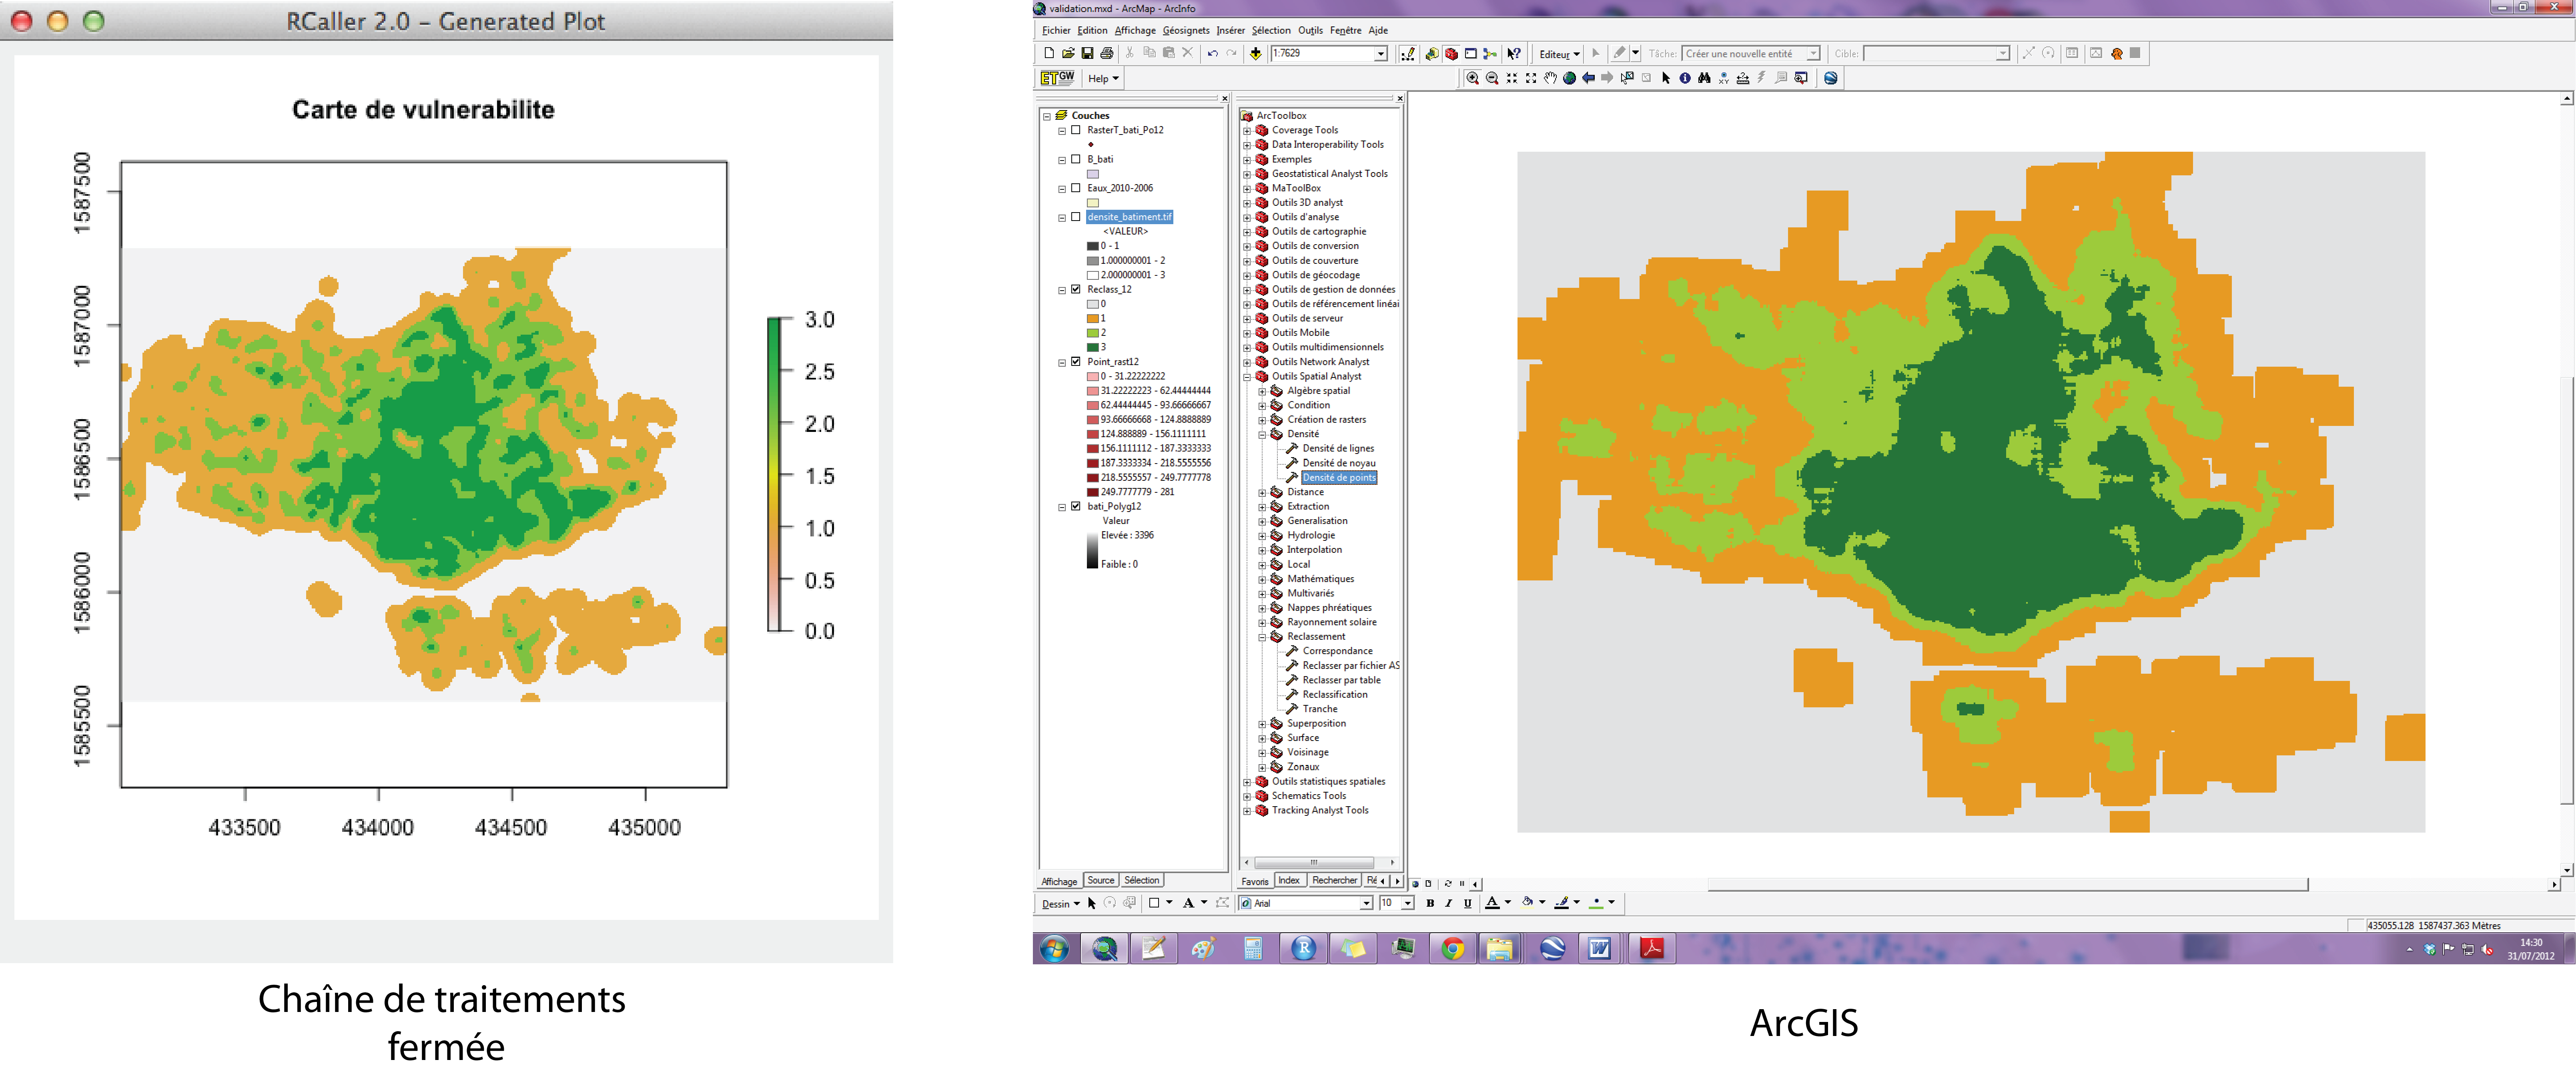
\includegraphics[width=14cm]{VulerabiliteComp}\\
\caption{\label{VulnerabComp} Cartes de vulnérabilté }
\end{figure}
\end{center}

Les deux cartes se ressemblent fortement. En analysant les statistiques des deux images raster générées, nous pouvons nous apercevoir que les résultats sont très similaires. \\
La carte générée à partir de la chaîne de traitements fermée présente les résultats suivants:
\begin{itemize}

\item Moyenne: 0.855 (valeur moyenne des cellules)
\item Ecart-type: 1.0249 (Ecart-type des cellules de l'image)\\

\end{itemize} 

La carte générée avec l'outil ArcGIS présente les résultats suivants:

\begin{itemize}

\item Moyenne: 0.9287 (valeur moyenne des cellules)
\item Ecart-type: 1.0461 (Ecart-type des cellules de l'image)\\

\end{itemize} 

Les différences entre les deux cartes sont donc minimes et comme l'aperçu des deux cartes est également très similaire nous pouvons donc valider le résultat de la carte de vulnérabilité.\\

Les petites différences peuvent être expliquées par le fait que ArcGIS et R (utilisé pour les calculs statistiques dans la chaîne de traitements fermée) utilisent des algorithmes différents pour effectuer les différentes calculs. Par exemple, lors du calcul de la densité des points, sous ArcgIS on a la possibilité de choisir entre plusieurs types de voisinage (rectangulaire, circulaire...). Nadine Dessay utilise le voisinage rectangulaire pour son travail. R et plus précisément le package "raster" utilise par défault un voisinage circulaire ce qui fait qu'en sortie les pixels des deux cartes ne sont pas identiques (rectangulaire sous ArcGIS et circulaire sous R).


\paragraph{Carte d'aléa\\\\}

\begin{center}
\begin{figure}[h] \centering
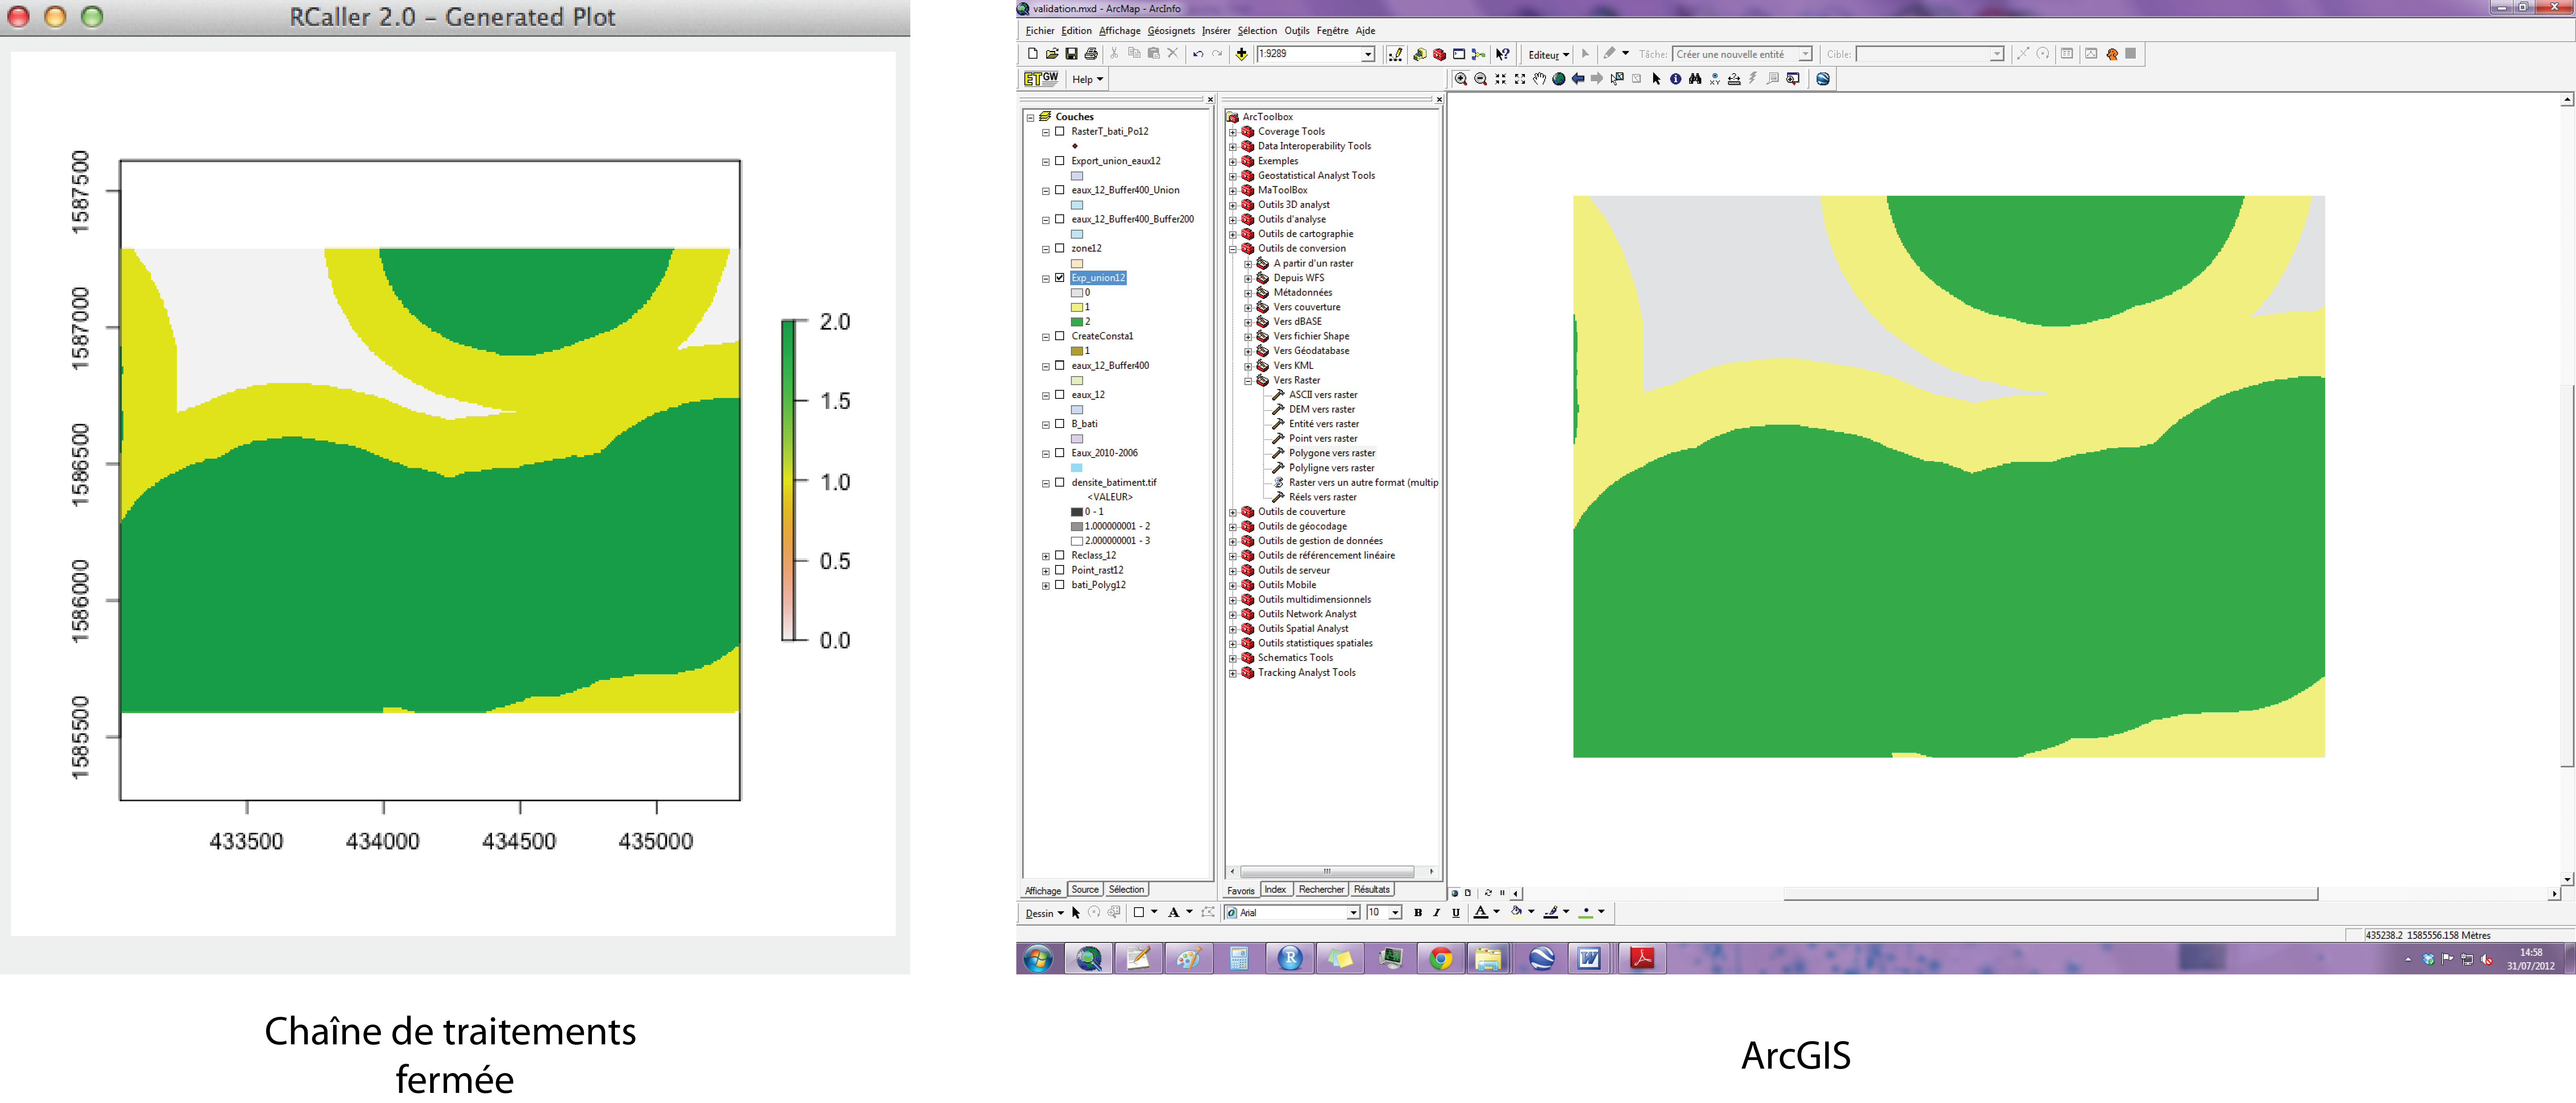
\includegraphics[width=14cm]{AleaComp}\\
\caption{\label{AleaComp} CArtes d'aléa}
\end{figure}
\end{center}

Pour l'élaboration de cette carte nous créons 2\textbf{ zones tampons} différentes: \\

Une zone tampon de 400 mètres autour des surfaces aquatiques. Sous ArcGIS, il existe la possibilité de créer par la suite une deuxième zone tampon autour de cette nouvelle couche créé (zones tampon de 400 mètres), dans notre cas de 200 m.\\
A l'intérieur de la chaîne de traitements cette opération est effectuée de la manière suivante: Création d'une zone tampon de 400 mètres et création d'une zone tampon de 600 mètres autour des surfaces aquatiques. \\
Par la suite nous créons une nouvelle donnée en soustrayant ces deux couches. Nous obtenons donc une couche correspondant à la zone tampon (200 mètres) autour de la zone de tampon de 400 mètres. \\
Comme on peut s'apercevoir en comparant les deux cartes (cf. \ref{AleaComp}), les résultats sont tout à fait identiques et nous pouvons valider le résultat de la chaîne de traitements fermée concernant la carte d'aléa.

\paragraph{Carte de risque\\\\}

\begin{center}
\begin{figure}[h] \centering
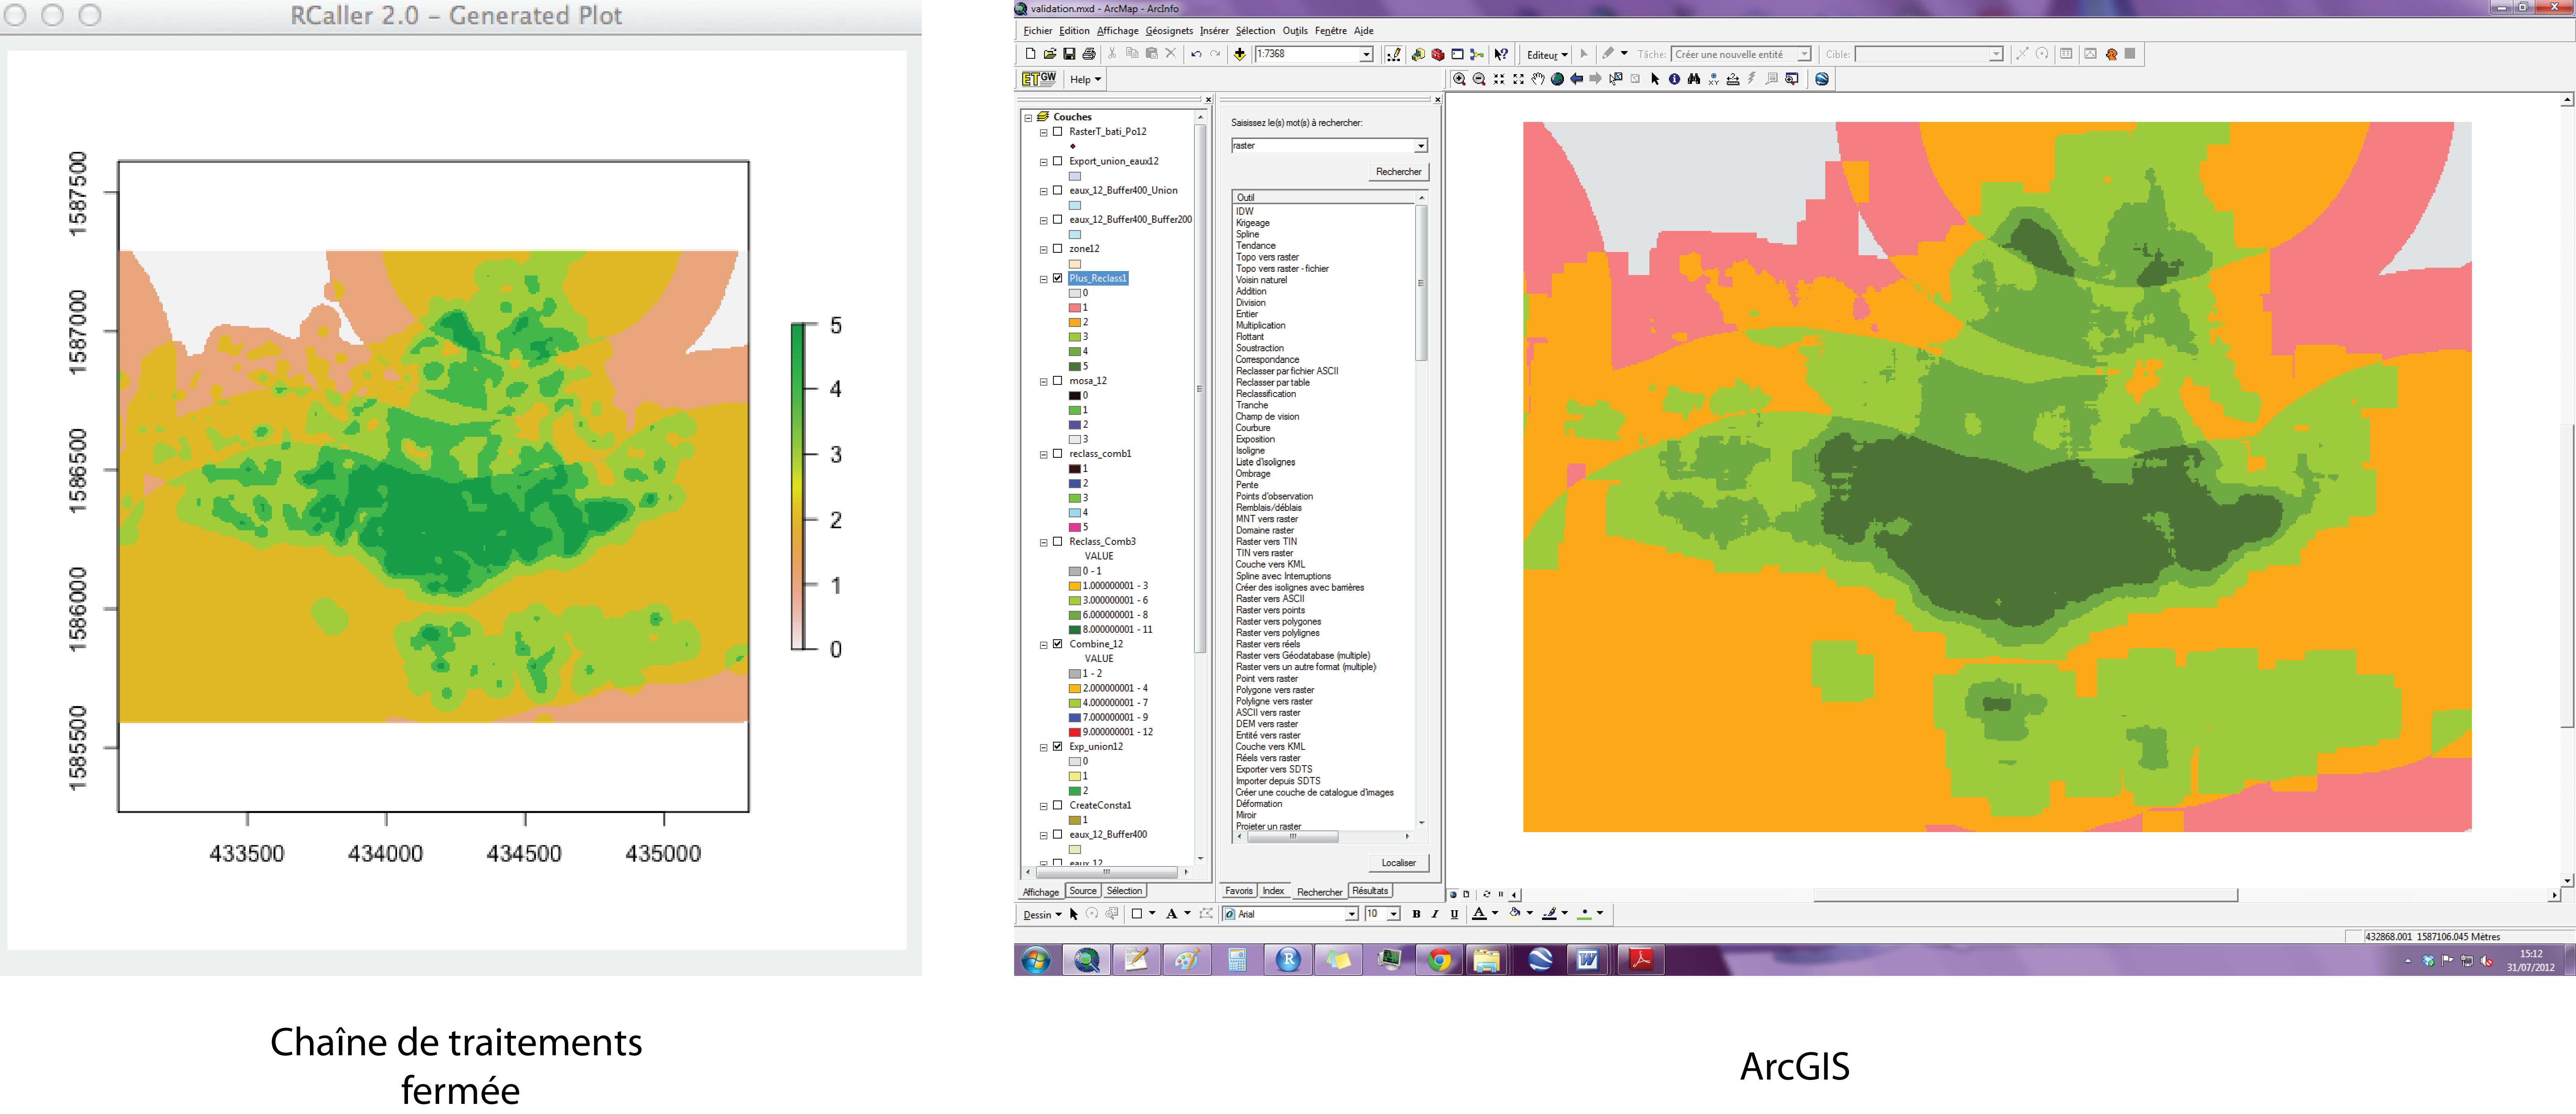
\includegraphics[width=14cm]{RisqueComp}\\
\caption{\label{RisqueComp} Cartes de risque}
\end{figure}
\end{center}

La carte de risque est obtenu est combinant la carte d'aléa et la carte de vulnérabilité. \\

Sous R, nous avons testé plusieurs possibilité pour effectuer ce genre d'opération. Nous avons obtenu le meilleur rendu en effectuons une addition des deux raster. Pour chaque pixel d'une image qui superpose avec un autre pixel d'une autre image, les valeurs des deux pixels sont additionnées.

Afin de valider cette approche, nous avons effectué la même opération sous ArcGIS. Les deux cartes valident nos résultats car ils sont à nouveau très similaires. 

\section{Difficultés rencontrées}

Tout au long du développement informatique de la chaîne de traitements et du logiciel ouvert, nous avons été confrontés à de nombreuses difficultés. Dans cette partie j'expliquerai les problèmes majeurs afin de faciliter le futur développement informatique de l'outil. Les difficultés sont regroupées en trois sous-parties : Difficultés liées au développement en Java, difficultés liées à l'utilisation de PostgreSQL / PostGIS et difficultés liées au logiciel R.\\

\subsection{Java}

Sur internet, il existe un nombre infini de forum et de tutoriels sur tout ce qui est programmation en Java. Ainsi, j'ai pu acquérir de nouvelles connaissances dans ce domaine. Néanmoins ce qui a été très compliqué, était de comprendre le fonctionnement de Rcaller, permettant d'utiliser les fonctionnalités de R sous Java. Il existe en effet que très peu de documentations et informations sur internet pour cette extension de Java. \\
La prise en main de Rcaller a nécessité un certain temps. Par exemple, nous avons dû faire face au problème que lors de l'affichage d'une donnée (plot), la fermeture d'une fenêtre causait automatiquement la fermeture de tout le programme. Pour résoudre ce problème, le résultat (l'image affichée) doit être stocké temporairement et par la suite être affiché dans une nouvelle fenêtre. \\
Une autre difficulté a été de comprendre comment intégrer des variables Java dans le code "R". Par exemple, en ce qui concerne la reclassification d'une image raster, l'utilisateur peut choisir le nombre de classes et les valeurs minimales et maximales de chaque classe. La commande "addDoubleArray" de RCaller permet d'intégrer un tableau composé de valeurs du type double dans le code R. En fonction des choix de l'utilisateur, Rcaller crée à l'intérieur du code R une "matrice" comportant les valeurs du tableau Java. \\

Il est également possible de récupérer les résultats de calculs effectués dans R. On peut seulement récupérer le résultat de la dernière ligne du code R. Par exemple, si on calcule deux moyennes différentes, il est nécessaire de stocker les deux moyennes dans une "liste" (moyenne <- list(moyenne1,moyenne2) sous R). Avec la commande "runAndReturnResult (moyenne)" il est par la suite possible de récupérer le résultat des calculs stocké dans la liste "moyenne".\\

Ces illustrations rendent compte très partiellement des nombreuses difficultés que nous avons rencontrées en utilisant RCaller. Finalement il faut aussi préciser que l'exécution de cette extension est en général très lente, notamment si l'utilisateur ne dispose pas d'une machine performante.

\subsection{PostgreSQL/PostGIS}

En ce qui concerne l'utilisation de PostGIS et de PostgreSQL, ce qui a été le plus compliqué était certainement l'installation. Lorsque nous avons démarré le développement informatique de la chaîne de traitements, nous utilisions une version antérieure de PostgreSQL et de PostGIS. Le 3 avril 2012 est sortie PostGIS 2.0 avec comme principale nouveauté la gestion des images rasters. Le passage à la nouvelle version a été assez compliqué, notamment sous le système d'exploitation Linux. En effet, toutes les librairies utilisées par PostGIS comme GDAL, PROJ etc. ont dû être mises à jour, tout comme la version de PostgreSQL (minimum 8.4). Sous Windows et MacOS ceci a posé moins de problèmes car des exécutables d'installation sont disponibles sur internet et les anciennes versions peuvent être supprimées plus facilement.\\

Souvent il n'est pas possible d'effectuer des opérations sur des données spatiales stockées dans la base de données, probablement parce qu'il y a eu un problème de type de géométrie lors de la construction de la donnée. Pour résoudre ce problème, il ést nécessaire pour chaque traitement PostGIS (par exemple Intersection entre deux couches) de créer une donnée "temporaire" à l'aide la fonctionnalité PostGIS "ST\_Buffer". Cette fonctionnalité crée théoriquement des zones tampons. En créant des zones de tampons de taille zéro, la fonctionnalité permet également de résoudre ce genre de problème.\\
% regarder les fonctions de détéction et transformation de types 


\subsection{R}

Par rapport à l'utilisation de R, nous avons été confronté à une difficulté majeure qui est l'utilisation de la librairie "rgdal". Sous Linux, il a été assez facile d'installer cette libraire à l'aide de la commande R "install.packages("rgdal")", néanmoins il est important de vérifier que lors de l'installation les versions de GDAL, PROJ et GEOS soient mises à jour car sinon un certain nombre de fonctionnalités risque de ne pas fonctionner. \\

Sous MacOS, il est nécessaire de faire l'installation à partir de la  source du package. Sur le site \url{http://www.r-bloggers.com/installing-rgdal-on-mac-os-x-2/} sont expliquées les informations nécessaires pour cette opération.\\

Sous Windows, l'installation de rgdal est facile et se fait à l'aide de la commande "install.packages". Malheureusement, il est impossible d'influencer la version GDAL utilisée lors de l'installation du package. Ainsi, il est actuellement impossible de charger des données dans R à partir d'une base de données PostgreSQL en utilisant rgdal. Ainsi, sous Windows, la chaîne de traitements ne fonctionne pas encore et le logiciel libre présente des fonctionnalités limitées (tous les traitements liés à l'utilisation de R ne fonctionnent pas).\\


\section{Perspectives}

L'objectif principal du stage était la conceptualisation et le développement informatique d'une chaîne de traitements permettant de cartographier le risque de transmission du paludisme. La définition des facteurs de risque de transmission du paludisme a été une première étape indispensable de ce travail.\\

Le modèle conceptuel ainsi que les listes concernant les différents facteurs de risque de transmission permettent aux experts, mais également à des non-experts, de comprendre les éléments  du cycle du paludisme et comment le paludisme se développe.\\

A partir de ce modèle conceptuel, nous avons pu définir les traitements nécessaires pour cartographier le risque. Par la suite,  de nombreuses réflexions autour de l'architecture informatique ont été menées. L'objectif était que la chaîne soit réutilisable pour le plus grand nombre de personnes. Créer un logiciel basé sur une architecture OpenSource et libre était donc indispensable. Nous avons décidé de développer la chaîne en Java. Par la suite, nous avons recherché pour chaque traitement les libraires et outils nécessaires. Très rapidement, nous nous sommes aperçus que PostgreSQL, PostGIS (traitements d'analyse spatiale) et R (notamment pour les traitements statistiques et les traitements raster) permettent d'effectuer tous les traitements que nous devions enchaîner.\\

Au bout de quatre mois, le développement informatique a abouti à une première chaîne de traitements fermée. Cette chaîne de traitements effectue un certain nombre de traitement dans un ordre bien précis, l'utilisateur n'a aucune influence sur le déroulement des traitements.\\

Avec les différents encadrants (et comme le travail avait avancé plus vite que prévu), nous avons décidé qu'il serait intéressant de développer, en se basant sur les traitements de la chaîne de traitements, un logiciel qui permettra d'effectuer chaque traitement indépendamment.\\

Le logiciel qui a été développé permet d'imaginer de nombreuses perspectives. A court terme, il peut être très intéressant de faire évaluer l'outil et de bien sûr rédiger un mode d'emploi pour l'outil et relever les retours des utilisateurs. D'ores et déjà, nous pensons qu'il serait bien  d'améliorer l'affichage des données (avec Grass par exemple) et d'améliorer la gestion des couches dans la base. La possibilité de se connecter à une base de données externe (hébergé sur un serveur internet) permet aussi d'envisager l'utilisation de l'outil dans de nombreux projets. Beaucoup de gens sont intéressés par les fonctionnalités de PostGIS, mais ne disposent pas des connaissances nécessaires pour son utilisation. Le logiciel leur permet dans un premier temps de créer une base de données, d'insérer des vecteurs et des rasters dans cette base et d'effectuer un certain nombre de traitements sur ces données. A long terme, l'intégration de nouveaux traitements pourrait faire de ce logiciel un outil précieux pour les gens souhaitant d'effectuer des traitements d'analyse spatiale de base (intersection, union, zones tampon etc.).

A long terme, il peut être envisagé de créer un équivalent du  "ModelBuilder" d'ArcGIS. L'utilisateur pourrait donc créer ses propres chaînes de traitements en fonction de ses besoins. En plus, il est alors envisageable que ces chaînes soient capitalisables et réutilisables.

\section{Conclusion}

Au terme des six mois de stage, la collaboration avec des experts dans des domaines divers (informatique, environnement, environnement-santé, biologie etc.) m'a permis d'acquérir un grand nombre de connaissances et de compétences et de travailler sur une multitude de thématiques.\\

L'élaboration d'un modèle conceptuel autour des éléments du paludisme a nécessité une recherche bibliographique importante ainsi qu'une longue phase de réflexion. Ce travail m'a donc surtout apporté beaucoup sur le plan scientifique.\\

Dans un deuxième temps, le développement respectivement d'une chaîne de traitements fermée et d'un logiciel ouvert m'a permis d'approfondir mes connaissances dans plusieurs domaines de l'informatique : Gestion des bases de données (spatiales), R et surtout programmation en Java sans oublier bien évidemment la conceptualisation et toutes les étapes de réflexion de la chaîne en amont.\\

Toutes les étapes, les erreurs et les leçons tirées de ce stage m'ont beaucoup aidé à évoluer dans le monde des SIG et plus particulièrement dans le domaine de l'informatique.\\

La qualité des résultats obtenus avec la chaîne de traitements fermée comparéé à celle des résultats obtenus à partir d'ArcGIS démontre les capacités des outils développés dans le cadre de ce travail et des outils et librairies libres et gratuites comme PostGIS/PostGreSQL et R. Les outils peuvent intéresser beaucoup de personnes, non seulement en ce qui concerne la cartographie de risques environnementaux, mais également pour effectuer des traitements d'analyse ou pour gérer et créer des bases de données spatiales. La possibilité de se connecter à une base de données distante est certainement un des atouts de cet outil.

Finalement, les objectifs du stage ont été atteints. La chaîne de traitements fermée est opérationnelle. Le logiciel ouvert permet, quant à lui, d'effectuer chacun des traitements de manière indépendante. 



\chapter{Discussion}






\chapter{Glossaire et définitions}
\label{Glossaire}

\textbf{API} : En informatique, une interface de programmation (souvent désignée par le terme API pour Application Programming Interface) est un ensemble normalisé de classes, de méthodes ou de fonctions qui sert de façade par laquelle un logiciel offre des services à d'autres logiciels. Elle est offerte par une bibliothèque logicielle ou un service web, le plus souvent accompagnée d'une description qui spécifie comment des programmes consommateurs peuvent se servir des fonctionnalités du programme fournisseur.

Des logiciels tels que les systèmes d'exploitation, les systèmes de gestion de base de données, les langages de programmation, ou les serveurs d'applications comportent une interface de programmation\footnote{\url{http://fr.wikipedia.org/wiki/Interface_de_programmation}}.\\

\textbf{Eclipse} : L'environnement de programmation (IDE) en langage Java le plus connu est le projet "Eclipse" de la fondation Eclipse. Ce logiciel simplifie la programmation grâce à un certain nombre de raccourcis et notamment grâce à la possibilité d'intégrer de nombreuses extensions. Au fur et à mesure de l'avancement du code, Eclipse compile automatiquement le code et signale les problèmes qu'il détecte.\\

\textbf{Géomatique} : La géomatique est la combinaison syntaxique de deux mots : Géographie et Informatique.
Le mot géomatique a été déterminé pour regrouper de façon cohérente l’ensemble des connaissances et technologies nécessaires à la production et au traitement des données numériques décrivant le territoire, ses ressources ou tout autre objet ou phénomène ayant une position géographique.
La géomatique est un domaine qui fait appel aux sciences, aux technologies de mesure de la terre ainsi qu’aux technologies de l’information pour faciliter l’acquisition, le traitement et la diffusion des données sur le territoire (aussi appelées "données spatiales ", "données géospatiales" ou " données géographiques").
La géomatique est étroitement liée à l’information géographique qui est la représentation d’un objet ou d’un phénomène localisé dans l’espace.
Ainsi, la géomatique regroupe l’ensemble des outils et méthodes permettant de représenter, d’analyser et d’intégrer des données géographiques
\footnote{\url{http://www.sig-geomatique.fr/sig-geomatique.html}}.\\

\textbf{Java} : Java est un langage orienté objet, c'est-à-dire que le programme est vu comme un ensemble d'entités (de classes). Au cours de l'exécution du programme, les entités collaborent entre elles pour arriver à un but commun.\\

\textbf{POM} : Chaque projet ou sous-projet est configuré par un POM "Project Object Model" qui contient les informations nécessaires à Maven pour traiter le projet (nom du projet, numéro de version, dépendances vers d'autres projets, bibliothèques nécessaires à la compilation, noms des contributeurs etc.). Ce POM se matérialise par un fichier pom.xml à la racine du projet. Cette approche permet l'héritage des propriétés du projet parent. Si une propriété est redéfinie dans le POM du projet, elle recouvre celle qui est définie dans le projet parent. Ceci introduit le concept de réutilisation de configuration. Le fichier pom du projet principal est nommé pom parent. Il contient une description détaillée de votre projet, avec en particulier des informations concernant le versionnage et la gestion des configurations, les dépendances, les ressources de l'application, les tests, les membres de l'équipe, la structure et bien plus.\\

\textbf{PostgreSQL} : PostgreSQL est un système de gestion de bases de données relationnelles objet (Manuel PostgreSQL). PostgreSQL est un outil Open Source et disponible gratuitement, compatible avec les systèmes d'opérations les plus connus (Linux, Unix (Mac OSX, Solaris etc.) et Windows). PostgreSQL propose des interfaces de programmations pour des langages de programmation comme Java, C++, Python etc.
Le développement de PostgreSQL a débuté en 1986 (appelé à l'époque Postgres). En 1995, les développeurs ajoutent un interpréteur de langage SQL à l'outil. A partir de 1996, l'outil s'appelle PostgreSQL afin de souligner le lien entre Postgres et le langage SQL. PostgreSQL peut être facilement étendu par l'utilisateur en ajoutant de nouvelles fonctions, de nouveaux opérateurs ou même de nouveaux langages de procédure.\\

\textbf{PostGIS} : PostGIS est une extension du système de gestion de base de données PostgreSQL qui permet de stocker des données (objets) géographiques dans la base de données. Cette extension permet d'utiliser une base de données PostgreSQL comme une base de données dans n'importe quel projet SIG. PostGIS est compatible avec de nombreux autres outils SIG comme par exemple QGIS, Mapserver, etc...\\

\textbf{REST} : REST "Representational State Transfer" (REST) ​​est un style d'architecture logicielle comprenant des lignes directrices et des meilleures pratiques pour la création de services Web évolutifs. REST est un ensemble coordonné de contraintes appliqué à la conception de composants dans un système hypermédia distribué qui peut conduire à une architecture plus performante et maintenable.

REST a gagné sa réputation à travers le web comme une alternative plus simple à SOAP et des services basés sur un WSDL. Les systèmes "RESTful" peuvent généralement, mais pas toujours, communiquer avec les verbes du protocole HTTP (GET, POST, PUT, DELETE, etc.) utilisés par les navigateurs Web pour récupérer des pages Web et envoyer des données à des serveurs distants.\\


\textbf{SAAS} : SAAS "Software as a Service" Le logiciel en tant que service est un modèle d'exploitation commerciale des logiciels dans lequel ceux-ci sont installés sur des serveurs distants plutôt que sur la machine de l'utilisateur. Les clients ne paient pas de licence d'utilisation pour une version, mais utilisent généralement gratuitement le service en ligne ou payent un abonnement récurrent\footnote{\url{http://fr.wikipedia.org/wiki/Logiciel_en_tant_que_service}}.\\

\textbf{SoapUI} : SoapUI est outil graphique qui permet de tester des services web basés sur diverses technologies. Il est disponible en deux versions : une version gratuite et open source et seconde version payante. Il est également disponible sous forme de plugin pour les IDE Netbeans, IntelliJ IDEA et Eclipse. SoapUI est développé entièrement en Java et utilise Java Swing pour son GUI, il fonctionne donc sur la plupart des systèmes d'exploitation et en plus il est disponible sous licence GNU.
L'outil gère respectivement les services web basés sur les technologies telles que le HTTP (S), HTML, SOAP (WSDL), REST, AMF, JDBC et JMS.\\

\textbf{SVN} : SVN ou Subversion est un système de gestion de version, conçu pour remplacer CVS. Concrètement, ce système permet aux membres d’une équipe de développeur de modifier le code du projet quasiment en même temps. Le projet est en effet enregistré sur un serveur SVN et à tout moment, le développeur peut mettre à jour une classe avant de faire des modifications pour bénéficier de la dernière version et a la possibilité de comparer deux versions d'un même fichier.\\

\textbf{WS} : Acronyme de "Web Service" ou Service Web. Un WS est un programme informatique de la famille des technologies web permettant la communication et l'échange de données entre applications et systèmes hétérogènes dans des environnements distribués. Il s'agit donc d'un ensemble de fonctionnalités exposées sur internet ou sur un intranet, par et pour des applications ou machines, sans intervention humaine, de manière synchrone ou asynchrone. Actuellement, le protocole de transport est essentiellement HTTP(S)\footnote{\url{http://fr.wikipedia.org/wiki/Service_web}}. \\



\chapter{Annexes}
\label{Annexes}

\section{Apache Maven}\label{Annexe A}\\

\textbf{Apache Maven} est un outil pour la gestion et l'automatisation de production des projets logiciels Java en général et Java EE en particulier. L'objectif recherché est comparable au système Make sous Unix : produire un logiciel à partir de ses sources, en optimisant les tâches réalisées à cette fin et en garantissant le bon ordre de fabrication.\\
Il est semblable à l'outil Ant, mais fournit des moyens de configuration plus simples, eux aussi basés sur le format XML. Maven est géré par l'organisation Apache Software Foundation. Précédemment Maven était une branche de l'organisation Jakarta Project.\\
Maven utilise un paradigme connu sous le nom de Project Object Model (POM) afin de décrire un projet logiciel, ses dépendances avec des modules externes et l'ordre à suivre pour sa production. Il est livré avec un grand nombre de tâches pré-définies, comme la compilation de code Java ou encore sa modularisation.\\
Un élément clé et relativement spécifique de Maven est son aptitude à fonctionner en réseau. Une des motivations historiques de cet outil est de fournir un moyen de synchroniser des projets indépendants : publication standardisée d'information, distribution automatique de modules « jar ». Ainsi en version de base, Maven peut dynamiquement télécharger du matériel sur des dépôts logiciels connus. Il propose ainsi la synchronisation transparente de modules nécessaires.\\

\pagebreak

\section{DropWizard}\label{Annexe B}\\

\textbf{Dropwizard} est un framework Java léger adapté au développement rapide de microservices REST et ne nécessitant pas de serveur d’application comme environnement d’exécution. \\
Cela dit, au delà du framework, c’est surtout un assemblage habile de composants spécialisés parmi les meilleurs de l’écosystème Java :
\begin{itemize}
\item \textbf{Jetty}, un serveur HTTP et un moteur de servlet compacts et très performants 
\item \textbf{Jersey}, l’implémentation de référence de la spécification JAX-RS (web services REST) 
\item \textbf{Jackson}, une librairie de sérialisation/dé-sérialisation JSON 
\item \textbf{Hibernate Validator}, l’implémentation de référence de l’API Bean Validation (JSR 303) 
\item \textbf{SLF4J} et \textbf{Logback} pour la gestion des traces 
\item \textbf{Metrics} pour le monitoring 
\item \textbf{jDBI} pour l’interfaçage rapide à une base de données relationnelle. Cette librairie est de bien plus bas niveau que JPA ou Hibernate et présente peu d’abstraction ce qui rend sa prise en main aisée \\
\end{itemize}

Packagée sous la forme d’un jar autonome contenant toutes ses dépendances, l’unité de déploiement n’a pas besoin de serveur d’application pour être exécutée (le conteneur Jetty est embarqué dans le jar). Avec ses 10 Mo tout au plus (dépendances comprises) l’empreinte mémoire d’une application Dropwizard est donc incomparablement plus faible qu’un Web Service SOAP déployé dans un serveur d’application Java EE (jusqu’à plusieurs centaines de Mo).
En conséquences, le temps de démarrage d’une application Dropwizard est de quelques secondes quand il faut parfois plusieurs minutes pour un serveur d’application.\\

\pagebreak


\section{Redmine}\label{Annexe C}

Redmine est considéré comme l’un des outils de gestion de projets collaboratifs Open Source parmi les plus aboutis. Il recouvre un ensemble de fonctionnalités dont un aperçu est donné ci-dessous, comme la gestion multi-projets, la gestion des demandes d’évolution et des bugs, la gestion et l’indexation des documentations techniques, mais aussi la gestion des droits et des profils des différents intervenants. Il propose aussi une console de suivi de l’état d’avancement des projets, des tâches, des recettes… sous forme de diagramme de Gantt.\\

Redmine est une forge logicielle sous licence GPL. Ses principaux concurrents se nomment Trac, Retrospectiva, Django Projector ou encore InDefero. Notons que Jira ne trouve pas sa place ici, bien qu’il soit le concurrent le plus sérieux de Redmine, parce que Jira est sous Dual licence (l’utilisation commerciale nécessite une licence payante non-Open Source).\\

Redmine offre un ensemble de fonctionnalités comme par exemples :

\begin{itemsize}
\item Prise en charge de plusieurs projets
\item Contrôle d’accès avec un modèle flexible de rôles
\item Gestion avancée des tickets
\item Diagramme de Gantt et calendrier
\item Publication de news, documents et gestionnaire de fichiers
\item Notifications par emails et flux ATOM
\item Wiki et forums par projet
\item Outil de suivi du temps
\item Champs personnalisables pour les tickets, suivi de temps, projets et utilisateurs
\item Intégration avec plusieurs SCM : SVN, CVS, Git, Mercurial, Bazaar et Darcs
\item Une communauté active et un ensemble d’outils connexes
\end{itemsize}\\

Plus de détails est disponible sur le wiki du projet : \url{http://www.redmine.org/projects/redmine/wiki}.

\pagebreak

\section{Extraits de codes}\label{Annexe D}\\

\textbf{Instanciation d'un objet upload}\\
\begin{lstlisting}
	// Instanciation
	Upload up = new Upload();
	up.setId(CreateUUID.randomUUID().toString());
	up.setOrganization(user.getOrganization());
	up.setName(fileDetails.getFileName());
\end{lstlisting} \\

\textbf{La classe Upload.java associée}\\

\begin{lstlisting}
	// Empty constructor
	public Upload (){
	}

    // Constructor
    public Upload(String id, String name, String uploadStatus, String organization, String uploadPath){
        super();
        this.id=id;
        this.name = name;
        this.uploadStatus = uploadStatus;
        this.organization = organization;
        this.uploadPath = uploadPath;
    }
    
    // Getters & Setters
    public String getId() {
        return id;
    }

    public void setId(String id) {
        this.id = id;
    }
    
    public String getName() {
        return name;
    }

    public void setName(String name) {
        this.name = name;
    }

    public String getUploadStatus() {
        return uploadStatus;
    }

    public void setUploadStatus(String uploadStatus) {
        this.uploadStatus = uploadStatus;
    }

    public String getOrganization() {
        return organization;
    }

    public void setOrganization(String organization) {
        this.organization = organization;
    }

    public String getUploadPath() {
        return uploadPath;
    }

    public void setUploadPath(String uploadPath) {
        this.uploadPath = uploadPath;
    }
	// suite des Getters & Setters
\end{lstlisting} \\

\textbf{Classe UploadDAO.java}\\

\begin{lstlisting}
	// Create 
    public String create(Upload up)
    {
        System.out.println("Upload instance created : "+up.getId()+" | "+up.getName()+" | "+up.getUploadStatus()+" | "+up.getOrganization()+" | "+up.getUploadPath());
        return persist(up).getId();
    }

    // Read one
    public Upload findByID(String id)
    {
        //return get(id);
        Query query = namedQuery("com.mobigis.dao.Upload.findByID");
        query.setParameter("id", id);
        List<Upload> res = list(query);
        if(res != null && res.size()>0)
        {
            return res.get(0);
        }
        return null;
    }
\end{lstlisting} \\


\textbf{Extrait du log Eclipse}\\

\begin{lstlisting}
INFO  [2015-06-11 15:31:52,883] com.mobigis.thread.AbstractUploadManagerThread: GTFS validation JSON report done !
file unzip : agency.txt
file unzip : calendar.txt
file unzip : calendar_dates.txt
file unzip : fare_attributes.txt
file unzip : fare_rules.txt
file unzip : frequencies.txt
file unzip : routes.txt
file unzip : shapes.txt
file unzip : stop_times.txt
file unzip : stops.txt
file unzip : trips.txt
Extract Done
Clean directory Done
upload status = UPLOADED
INFO  [2015-06-11 15:31:52,920] com.mobigis.thread.AbstractUploadManagerThread: Process upload to Location = C:\mobianalystserver\download\tisseo\gtfs\215b8557-f7c9-4b06-aced-f79bde953c65
INFO  [2015-06-11 15:31:52,920] com.mobigis.thread.AbstractUploadManagerThread: Upload file done ! Id = 215b8557-f7c9-4b06-aced-f79bde953c65 | Status = UPLOADED
C:\mobianalystserver\download\tisseo\gtfs\215b8557-f7c9-4b06-aced-f79bde953c65
INFO  [2015-06-11 15:31:52,965] org.hibernate.engine.internal.StatisticalLoggingSessionEventListener: Session Metrics {
    36877 nanoseconds spent acquiring 1 JDBC connections;
    0 nanoseconds spent releasing 0 JDBC connections;
    358836 nanoseconds spent preparing 4 JDBC statements;
    6286839 nanoseconds spent executing 4 JDBC statements;
    0 nanoseconds spent executing 0 JDBC batches;
    0 nanoseconds spent performing 0 L2C puts;
    0 nanoseconds spent performing 0 L2C hits;
    0 nanoseconds spent performing 0 L2C misses;
    24185654 nanoseconds spent executing 1 flushes (flushing a total of 2 entities and 2 collections);
    42650 nanoseconds spent executing 1 partial-flushes (flushing a total of 0 entities and 0 collections)
}
127.0.0.1 - - [11/Jun/2015:15:31:50 +0000] "POST /upload/gtfs HTTP/1.1" 200 61 "-" "Apache-HttpClient/4.1.1 (java 1.5)" 2254
\end{lstlisting} 


\pagebreak

\section{Structure d'une application Web}\label{Annexe E}\\


\begin{figure}[!h]
\centering
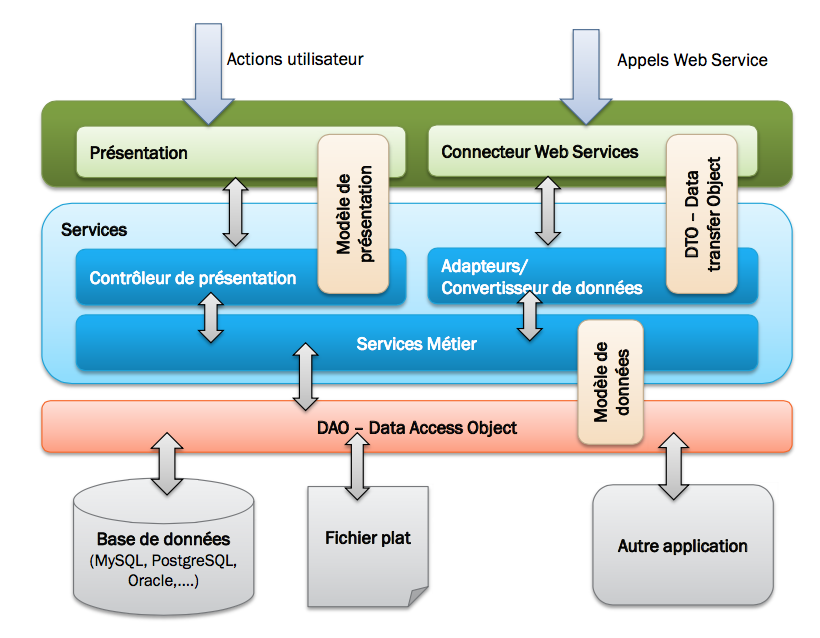
\includegraphics[width=\textwidth]{images/WebAppArchitecture.png}
\caption{\label{WebAppArchitecture}Structure d'une application Web}
\end{figure} 



%\chapter*{Webographie}
\label{Bibliographie}


\textbf{Sites sur les données/outils "métiers" :}\label{OBA}\\


\url{https://developers.google.com/transit/gtfs/examples/gtfs-feed}\\

\url{https://developers.google.com/transit/gtfs/}\\

\url{https://github.com/google/transitfeed/wiki/FeedValidator}\\

\url{http://onebusaway.org/developer-information/}\\

\url{https://github.com/OneBusAway/onebusaway/wiki/Importing-source-code-into-Eclipse}\\


\textbf{Sites sur les frameworks et outils utilisés :}\\


\url{http://www.objis.com/formation-java/tutoriel-formation-maven-2.html}\\

\url{http://mvnrepository.com/}\\

\url{https://github.com/bucharest-jug/dropwizard-todo}\\

\url{http://docs.jboss.org/hibernate/orm/4.3/manual/en-US/html/}\\

\url{http://www.tutorialspoint.com/hibernate/}\\

\url{http://blog.xebia.fr/2011/11/14/rest-java-serveur/}\\


Et pour finir, un grand merci à \url{http://www.mkyong.com/}, tout simplement.


\bibliographystyle{apalike-fr} % Le style est mis entre crochets.
\bibliography{RapportBiblio}

%\section{Principes généraux}

testt



\end{document}